
%文章相关
\usepackage[UTF8, heading = false, scheme = plain]{ctex}    %解决中文字体,不改变排版
\usepackage{geometry}                                       %调整页边距等
\usepackage{indentfirst}                                    %首行缩进
\usepackage[dvipsnames,svgnames]{xcolor}                    %颜色包:\color{}
\usepackage{enumitem}                                       %控制item的前置符号
\usepackage{adjustbox}                                      %控制文字大小和添加底纹


%图片宏包
\usepackage{graphicx}                                       %插入图片:\includegraphics{myimage.png}
\usepackage{float}
\usepackage{caption}
\usepackage{subcaption}

%数学相关
\usepackage{amsmath,amsthm}                                 %amsmath包应该在前
\usepackage{extarrows}                                      %使用长等号A \xlongequal{\quad\quad}B
\usepackage{cases}                                          %\begin{numcases}可以为方程编号
\usepackage{amssymb}                                        %\checkmark 打勾

%实用的内容说明包
\usepackage{hyperref}                                       %超链接插入包:\href{url}{name}
\usepackage{multirow}                                       %插入表格用到的宏包:\begin{tabular}{|c|c|},&分列,\\分行,\hline插入横线(第二个参数是列数)
\usepackage{listings}                                       %插入代码等:\begin{lstlisting}[breaklines=true,backgroundcolor=\color{lightgray},title=]
\usepackage{verbatim}                                       %使用 comment 环境进行注释


%物理包
\usepackage{physics}
\usepackage{xparse}                                         %physics需求的包
\usepackage{mhchem}                                         %输入原子核的表式\ce{^238_92U}

% \eval{}        根据括号内容的大小在右边添加合适的竖线A|          |         \dv[n]{f}{x}          n阶微分算符 derivative
% \abs{}         添加绝对值|A|                                |         \pdv[n]{f}{x}         n阶偏微分算符 partialderivative
% \norm{}        模||A||                                     |          \bra \ket \braket    左、右、内积
% \comm{}{}      对易子[A,B]                                  |          \op{}{}              外积(密度算符) outerproduct
% \anticomm{}{}  反对易子{A,B}                                |          \ev{<力学量>}{<态>}    期望 expectationvalue
% \vb{}          向量加粗字体                                  |          \mel{}{}{}           矩阵元 matrixelement
% \va{}          向量                                        |          \mqty                 生成矩阵,可跟{} () [] || &分列 \\分行 第一个表示外面无框
% \vu{}          单位向量                                     |         \qty                  合适大小的{}、()等,例如 \qty(x)
% \vdot          点乘                                        |
% \cross         叉乘                                        |
% \grad          梯度 gradient                               |
% \div           散度 divergenc                              |
% \curl          旋度                                        |
% \laplacian     拉普拉斯算符                                 |

%文本底纹实现
\usepackage{lipsum}                                         %该宏包是通过 \lipsum 命令生成一段本文,正式使用时不需要引用该宏包
\usepackage[strict]{changepage}                             %提供一个 adjustwidth 环境
\usepackage{framed}                                         %实现方框效果
%\usepackage{newtxtext}                                     %在macos会报错的一个包注释掉不影响使用
\usepackage{tcolorbox}                                      %文本底纹包,放在xcolor包后
                               
% environment derived from framed.sty: see leftbar environment definition
\definecolor{formalshade}{rgb}{0.95,0.95,1}% 文本框颜色
% ------------------******-------------------
% 注意行末需要把空格注释掉,不然画出来的方框会有空白竖线
\newenvironment{formal}{%
\def\FrameCommand{%
\hspace{-1em}%                                              %框的整体缩进
{\color{Green}\vrule width 0.3em}%                          %竖线颜色以及宽度
\colorbox{greenshade}%                                      %底纹颜色
}%
\MakeFramed{\advance\hsize-\width\FrameRestore}%
\noindent\hspace{-2em}%                                     %禁止第一段文本缩进
\begin{adjustwidth}{}{2em}%                                 %控制右边距        
\vspace{1.5em}%                                             %控制上边距
}
{%
\vspace{1.5em}\end{adjustwidth}\endMakeFramed%              %控制底边距
}%

\definecolor{greenshade}{rgb}{0.90,0.99,0.91}               %绿色文本框,竖线颜色设为 Green
\definecolor{redshade}{rgb}{1.00,0.90,0.90}                 %红色文本框,竖线颜色设为 LightCoral
\definecolor{brownshade}{rgb}{0.99,0.97,0.93}               %莫兰迪棕色,竖线颜色设为 BurlyWood


%使用Mathematica进行计算
%\usepackage{latexalpha2}
%/usr/local/texlive/texmf-local/tex/latex/local/latexalpha2
%直接使用wolfram代码
% \wolfram[<format>]{<code>}    \wolframgraphics[<format>]{<code>}{<filename>} 
%具体使用方法查看 latexalpha2.pdf


%预设
\geometry{a4paper,left=5em,right=5em,bottom=5em,top=5em}    %设置为a4paper最好,点击pacakge geometry 查看文档
\setlength{\parindent}{2em}                                 %2em(注意不支持rem)代表每一段的首行缩进两个字符,某一行不缩进时使用 \noindent

\hypersetup{hidelinks,colorlinks=true,
linkcolor=black,urlcolor=blue}                              %对hyperref 包进行预设

\newenvironment{slt}{\proof[\indent \bf 解 ]}{
\renewcommand{\qedsymbol}{}\endproof}                       %提供解环境
\newtheorem{thm}{定理}[section]                              %定义一个新的环境 thm, 命名为定理,以 节 开始编号
\newtheorem*{thm*}{定理}                                     %定义一个新的环境 thm, 命名为定理,无编号
\newtheorem{lemma}{引理}[section]                            %定义新环境 lemma,命名为引理,以 节 开始编号
\newtheorem*{lemma*}{引理}                                   %定义新环境 lemma,命名为引理,无编号
\newtheorem{corollary}{推论}                                 %定义新环境 corollary,命名为推理,有编号
\newtheorem*{corollary*}{推论}                               %定义新环境 corollary*,命名为推理,无编号
\renewcommand{\proofname}{ \qquad \bf 证明}                  %更改proof为中文证明,proof环境默认存在

%一些def
\def\thmindent{\setlength{\parindent}{5em}}                  %\thmindent
\def\pfindent{\setlength{\parindent}{5.5em}}                 %\pfindent
\def\clindent{\setlength{\parindent}{4em}}                   %clindent
\def\sdr{Schr\"{o}dinger}                                    %薛定谔名字
\def\intff{\int_{-\infty}^{+\infty}}                         %积分为(-\infty,+\infty)的积分
\def\ra{\rightarrow}                                         %右键头\ra
\def\lra{\Longrightarrow}                                    %长(双)右键头\lra
\def\lla{\Longleftarrow}                                     %长(双)左键头\lla
\def\llra{\Longleftrightarrow}                               %等价箭头\llra
\def\xlra{\xlongrightarrow{\quad\quad}}                      %超长右箭头
\def\xlla{\xlongleftarrow{\quad\quad}}                       %超长左箭头
\def\xlla{\xlongleftrightarrow{\quad\quad}}                  %超长等价箭头

\def\psii#1{\psi_{#1}}                                       %常用的\psi下标
\def\psiii#1#2{\psi_{#1} (#2)}                               %常用的\psi下标和括号
\def\psiiii#1#2#3{\psi_{#1}^{#2} (#3)}                       %常用的\psi下标、上标和括号
\def\pe#1#2{E_{#1}^{(#2)}}                                   %能量修正{下标}{上标}
\def\pp#1#2{\psi_{#1}^{(#2)}}                                %波函数修正
\def\ua{a_{+}}                                               %升算符
\def\da{a_{-}}                                               %降算符

\def\nuc#1#2#3{\ce{^{#1}_{#2}{#3}}}                          %原子核的表示形式


%其他备注
\begin{comment}
        求和指标上下方添加        \sum\limits_{}^{}
        恒等于                  \equiv
        远大于                  \gg
        远小于                  \ll
        花括号                  \left\{ \right\}   (建议使用\qty)
        弧度                    37^{\circ}


\end{comment}


%作业包(需要的时候再解除注释)
%\usepackage{iidef}
%建议使用自己的slt解环境
\begin{comment}

    package iidef:
        指定学校名      \thecourseinstitute{}      
        指定课程名      \thecoursename{} 
	    指定学期        \theterm{}
        作业名         \hwname{}
        生成作业标题    \courseheader           放在document环境内 不需要再maketile
        名字           \name                   放在document环境内
        自动编号环境    \begin{enumerate}       [label = (\alph*{})] [label = \arabic*{}.]
        题号           \item                   自动编号,\item[]则不带符号
        证明           \begin{proof}           证明环境由amsthm包提供
        求解           \begin{solution}       
        方程           \begin{equation}        
        方程编号        \labe{eq:[number]}      为方程设置编号  
        引用方程        \eqref{eq:[number]}     引用方程
        行内方程        $...$
        
        多行公式        \begin{align} \begin{align*}则不会编号  
                            ... & = ... \\ 
                                & = ...
                       \begin{array}{lcl}      
                            ... & = & ... \\ 
                            ... & = & ...
        
        方程组          $$
                        \begin{cases}
                       ... & \mbox{if} x \mbox{is even} \\ 带假设
                       $$
                       
                       带编号
                       \begin{numcases}{}
                            \label{1}   \\
                            \label{2}   
                       \end{numcases}
        
        文字大小和底纹
                       \vspace{-1em}
                       \begin{adjustbox}{minipage=0.91\linewidth, bgcolor=gray!20, padding=1em}
                       \small % 将字号变小为 small
                        text
                       \end{adjustbox}
                       \vspace{-1em}

        居中            不要使用$$...$$,会对齐失效 使用$...$即可
                        \begin{center}
            
                        \end{center}

        左对齐           
                        \begin{flushleft}
            
                        \end{flushleft}

        双水平图         \begin{minipage}{0.45\textwidth}
                        \includegraphics[width=\textwidth,keepaspectratio]{./pictures/.png}
                        \end{minipage}
                        \hfill
                        \begin{minipage}{0.45\textwidth}
                            \begin{enumerate}[label = (\arabic*)]
                                \item 
                                \item 
                                \item 
                            \end{enumerate}
                        \end{minipage}

    
\end{comment}




\title{量子力学习题集}
\author{马祥芸}

\begin{document}
    \maketitle
    \tableofcontents
    \newpage
    %\thecoursename{量子力学习题集}  %作业包页眉左边
    %\thecourseinstitute{马祥芸}    %作业包页眉右边

    \section{薛定谔方程与一维定态问题}

        \begin{formal}
            $$ \dv[2]{y}{x} + p\dv{y}{x} + qy = 0 $$
            
            特征根方程
            $$ r^{2} + pr + q = 0 $$

            \begin{enumerate}
                \item $r_{1} \neq r_{2}$且为实根
                $$ y = Ae^{r_{1}x} + Be^{r_{2}x} $$
                \item $r_{1} = r_{2}$且为实根
                $$ y = (C_{1}+C_{2}x)e^{r_{1}x} $$
                \item $r_{1}=\alpha + i \beta,r_{2} = \alpha - i \beta $为共轭复根(通常$\alpha$都是0)
                $$ y = e^{\alpha x} (C_{1}\cos{\beta x} + C_{2}\sin{\beta x}) \quad or \quad y = C_{1}e^{i\beta x} + C_{2}e^{-i\beta x}$$

                一阶微分变化值的关系
                $$ \triangle(\frac{d\psi}{dx}) = \int_{-\varepsilon}^{+\varepsilon}\frac{2\mu}{\hbar^2}V(x)\psi(x)dx $$    

                $\delta$函数性质

                $$\int_{-\varepsilon}^{+\varepsilon} \delta(x) \psi(x) dx =\psi(0) \quad \delta(Rx) = \frac{1}{R} \delta(x) $$

                常见三角函数的公式
                $$\sin(x+y)=\sin{x} \cos{y}+\sin{y}\cos{x} \quad \cos(x+y)=\cos{x} \cos{y} - \sin{x}\sin{y}$$ 
                $$\sin(2x) = 2\sin{x} \cos{x} \quad \cos(2x) = \cos^{2}{x} - \sin^{2}{x} $$
                $$\sin^{2}{x}=\frac{1-\cos(2x)}{2} \quad \cos^{2}{x}=\frac{1+\cos(2x)}{2} $$
                $$ 1 + \tan^{2}{x} = \frac{1}{\cos^{2}{x}} \quad \dv{\tan{x}}{x} = \frac{1}{\cos^{2}{x}} $$

                两个常见积分

                $$ \intff e^{-a (x+b)^{2}} dx = \sqrt{\frac{\pi}{a}} $$
                $$ \intff x^{2} e^{-a x^{2}} dx = \frac{1}{2a} \sqrt{\frac{\pi}{a}} $$

                动量表象问题
                $$ \psiii{p}{x} = \frac{1}{(2 \pi \hbar)^{\frac{n}{2}}} e^{\frac{ipx}{\hbar}} $$ 
                $$ \psiii{x}{p} = \frac{1}{(2 \pi \hbar)^{\frac{n}{2}}} e^{\frac{-ipx}{\hbar}} $$ 
                $$ \delta(x) = \frac{1}{(2\pi)^{n}} \intff e^{ipx} dp $$
                $$ \delta(p) = \frac{1}{(2\pi)^{n}} \intff e^{-ipx} dx $$
                $$ \psi(p) = \braket{p}{\psi} = \int dx' \braket{p}{x'} \braket{x'}{\psi} = \frac{1}{(2 \pi \hbar)^{\frac{n}{2}}} \intff \psi(x) e^{\frac{-ipx}{i\hbar}} dx $$
                $$ \psi(x) = \braket{x}{\psi} = \int dp' \braket{x}{p'} \braket{p'}{\psi} = \frac{1}{(2 \pi \hbar)^{\frac{n}{2}}} \intff \psi(p) e^{\frac{ipx}{i\hbar}}  dp $$

                海森堡绘景
                $$ \dv{A_{H}(t)}{t} = \pdv{A_{H}(t)}{t} + \frac{1}{i\hbar} [A_{H}(t),H] $$
                $$ \dv{<A_{H}(t)>}{t} = \pdv{<A_{H}(t)>}{t} + \frac{1}{i\hbar} \overline{[A_{H}(t),H]} $$

                概率流密度
                $$ j_{x} = \frac{1}{2} (\psi^{*} \vu*{v} \psi - \psi \vu*{v} \psi^{*} ) \quad \vu*{v} = \frac{\vu*{p}}{\mu} = - \frac{i\hbar}{\mu} \pdv{x} $$
                $$ T = \abs{\frac{j_{R}}{j_{I}}} \quad R = \abs{\frac{j_{T}}{j_{I}}} $$

                无限深方势阱([0,a]),归一化系数$A$,势阱长度$L$.
                $$ \psiii{n}{x} = \sqrt{\frac{2}{a}} \sin{\frac{n\pi x}{a}} \quad \frac{1}{2} L A^{2}  = 1 $$
                $$ E_{n} = \dfrac{n^{2}\pi^{2}\hbar^{2}}{2\mu a^{2}} $$

                谐振子
                $$ \psiii{n}{\xi} = N_{n} H_{n}(\xi) e^{-\frac{\xi^{2}}{2}} $$
                $$ N_{n} = \sqrt{\frac{\alpha}{\sqrt{\pi}2^{n} n!}}  \quad \alpha = \sqrt{\frac{\mu \omega}{\hbar}} \quad \xi = \alpha x $$
                $$ \psiii{0}{\xi} = \sqrt{\frac{\alpha}{\sqrt{\pi}}} e^{-\frac{\xi^{2}}{2}} \quad (H_{0}(\xi) = 1)$$
                $$ \psiii{1}{\xi} = \sqrt{\frac{\alpha}{\sqrt{\pi}}} \sqrt{2} \xi e^{-\frac{\xi^{2}}{2}} \quad (H_{1}(\xi) = 2\xi) $$
                
                $\qquad$谐振子波函数具有宇称$(-1)^{n}$,通常用于奇函数的积分性质,根据维里定理
                $$  < T > \quad = \quad  < V >  $$
                
                $\qquad$能量与升降算符
                $$ E_{n} = (\vu*{N} + \frac{1}{2}) \hbar \omega = (n + \frac{1}{2}) \hbar \omega   \quad  \vu*{N} = \ua \da   $$
                $$ \vu*{a}_{\pm} = \frac{1}{\sqrt{2\mu \hbar \omega}} (\mp i\vu*{p} + x) \quad \comm{\da}{\ua} = 1 $$
                $$ \ua \ket{n} = \sqrt{n+1}\ket{n+1} \quad \da\ket{n} = \sqrt{n}\ket{n-1} \quad \vu*{N}\ket{n} = n \ket{n}$$
                
                $\qquad$交叉相谐振子处理方式
                $$ \xi = \frac{1}{\sqrt{2}} (x+y) \quad \eta = \frac{1}{\sqrt{2}} (x -y)  $$
                $$ \xi^{2} + \eta^{2} = x^{2} + y^{2} \quad xy = \frac{1}{2} (\xi^{2} - \eta^{2}) \quad \pdv[2]{x} + \pdv[2]{y} = \pdv[2]{\xi} + \pdv[2]{\eta}$$
                
                $\qquad$其他性质
                $$  
                x \psi_{n} = \frac{1}{\alpha}(\sqrt{\frac{n}{2}}\psi_{n-1} + \sqrt{\frac{n+1}{2}} \psi_{n+1})  \quad 
                \dv{\psi_{n}}{x} = \alpha (\sqrt{\frac{n}{2}}\psi_{n-1} - \sqrt{\frac{n+1}{2}} \psi_{n+1}) 
                $$



                
                

                
            \end{enumerate}
        \end{formal}

        \subsection{一维有限势场}
        \begin{thm}\label{thm:1.1}                                                %添加\lable{书签名}进行标记,使用\pageref{书签名}添加标记位置的页码 \ref{书签名}引用定理编号
            势函数具有偶对称$V(x)=V(-x)$,$\psi(x)$和$\psi(-x)$均是波函数的解
            
            \begin{proof}
                
                $$ \frac{d^2}{[d(-x)]^2}=\frac{d^2}{dx^2} $$ 

            \end{proof}
        
        \end{thm}
    

        \begin{thm}\label{thm:1.2}
            \thmindent
            
            设$V(x)=V(-x)$,\textbf{每一个}$\psi(x)$都有确定的宇称(奇偶性)(注意每一个解的宇称可以不相同)
            
            \begin{proof}
                \pfindent
                
                由于定理\ref{thm:1.1},构造 
                   
                    $$ f(x) = \psi(x)+\psi(-x) $$                          % $$行公式不带编号
                    $$ g(x) = \psi(x)-\psi(-x) $$
                
                $f(x)$为偶宇称,$g(x)$为奇宇称,它们均为能量$E$的解       \par  %另起段落保留缩进
                而$\psi(x)$与$\psi(-x)$都可以用$f(x)$和$g(x)$表示    

                $$ \psi(x) = \frac{1}{2} [f(x)+g(x)]  $$
                $$ \psi(-x) = \frac{1}{2} [f(x)-g(x)] $$    

           \end{proof}
           
           \begin{corollary}\label{cl:1}
                \clindent 
                
                设$V(-x) = V(x)$,而且对应于能量本征值E,方程的解无简并,则该能量本征态必有确定的宇称,例如一维 \par
                谐振子,一维对称方势阱
                
                \begin{itemize}
                    \item 若$E$非简并  \quad 本征函数具有确定宇称(两种宇称) 
                        $$ \psi(-x) = \hat{P}\psi(x) = c\psi \quad c=\pm 1 $$ %\hat{}输入算符的帽子
                    \item 若$E$简并 \quad $\psi(x)$和$\psi(-x)$分别为独立的波函数,它们的线性组合是具有宇称的解
                        $$ \psiii{\pm}{x} = \frac{1}{\sqrt{2}}[\psi(x) \pm \psi(-x)] $$
                \end{itemize}
            
           \end{corollary}

        \end{thm}
        \par
        偶宇称涉及到的函数图像如下

        \begin{figure}[H]
            \centering
            \begin{subfigure}{0.48\textwidth}
                    
                \centering
                \wolframgraphics[png]{Plot[y=Tan[x],{x,0,2.5}]}{tanx}
                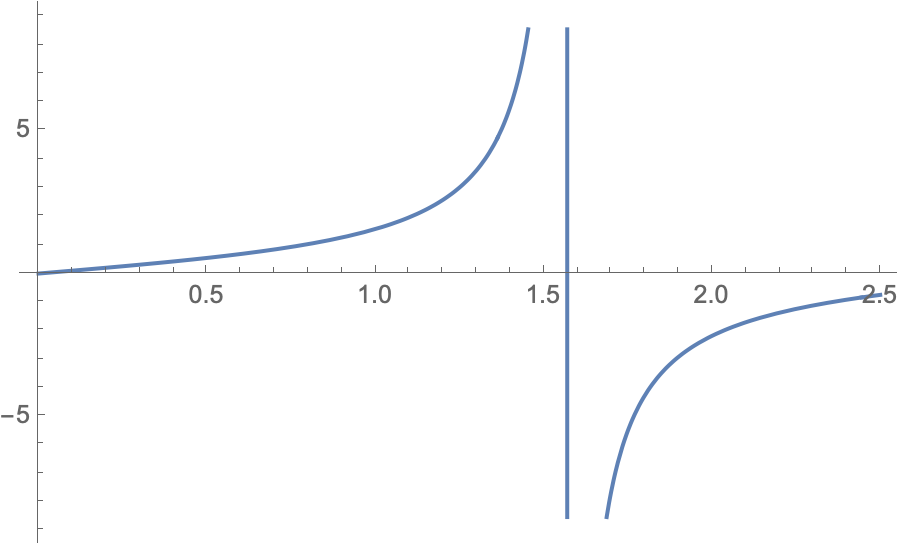
\includegraphics[scale=0.4]{tanx.png}
                \caption{$y=\tan{x}$}
                
            \end{subfigure}
            \begin{subfigure}{0.48\textwidth}
                
                \centering
                \wolframgraphics[png]{Plot[y=x*Tan[x],{x,0,2.5}]}{xtanx}
                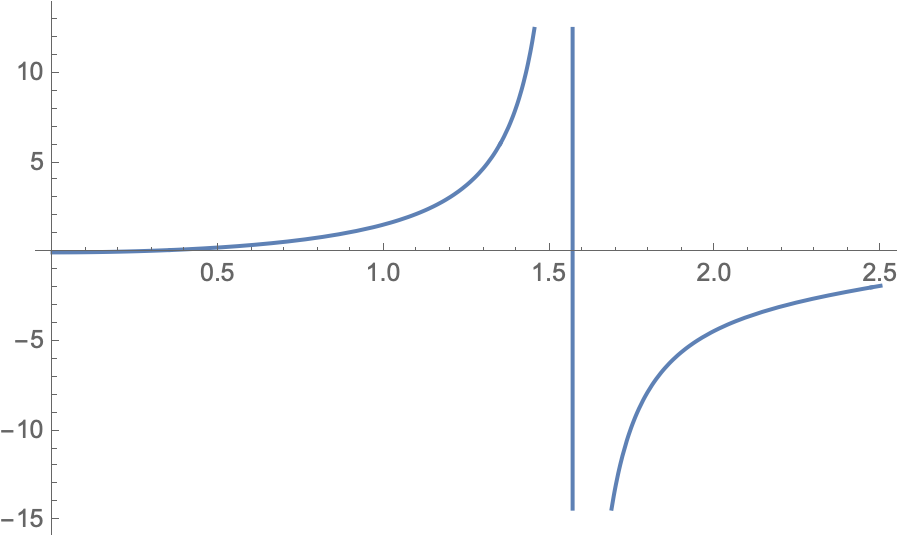
\includegraphics[scale=0.4]{xtanx.png}
                \caption{$y=x \tan{x}$}

            \end{subfigure}
              
        \end{figure}

        奇宇称涉及到的函数图像如下
        \begin{figure}[H]
            \centering
            \begin{subfigure}{0.48\textwidth}
                    
                \centering
                \wolframgraphics[png]{Plot[y=-x*Cot[x],{x,0,2.5}]}{-xcotx}
                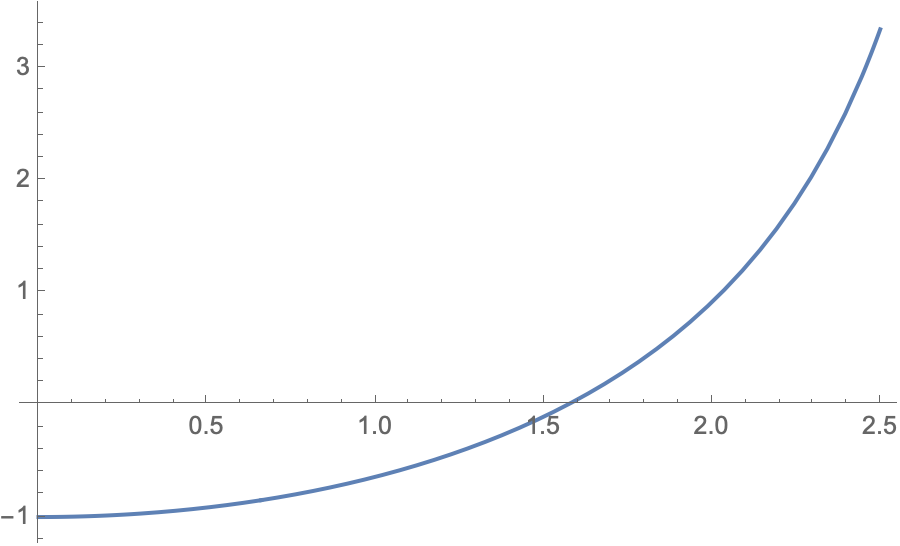
\includegraphics[scale=0.4]{-xcotx.png}
                \caption{$y=-x \cot{x}$}
                
            \end{subfigure}
            \begin{subfigure}{0.48\textwidth}
                
                \centering
                \wolframgraphics[png]{Plot[{y=-x*Cot[x],y=x*Tan[x],y=Sqrt[4-x^2]},{x,0,2.5}]}{3plot}
                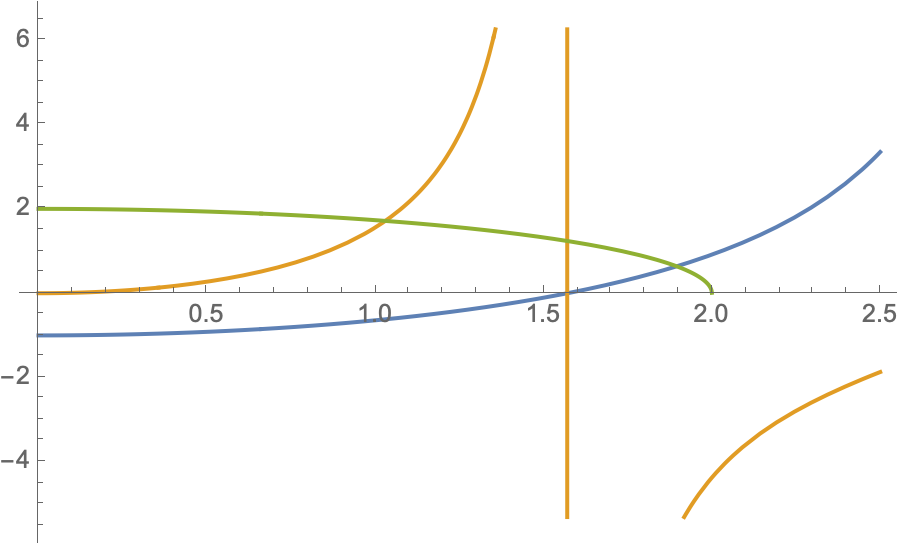
\includegraphics[scale=0.4]{3plot.png}
                \caption{三个函数曲线}

            \end{subfigure}
              
        \end{figure}

            %两个subfigure之间不能存在空行否则会出现竖排列

            
        
        由于此题的势能函数具有偶对称,因此波函数可能存在偶or奇宇称(需要分开讨论),此题中偶宇称至少存在一个交点,
        而奇宇称有解必须有条件$Q>\frac{\pi}{2}$,由题意可知存在且仅存在一个束缚态,所以保留偶宇称的唯一解即可($Q<\frac{\pi}{2}$)
        
        \subsection{一维 \texorpdfstring{$\delta$}{}势}   %使用\texorpdfstring{}{}来包括tex公式或者string需要两个参数或者仅用一个括号并用.连接
        
        先不考虑$x\neq0$的局部区域,丢掉$\delta(x)$势阱,需要用到  
        \begin{formal}
            
            \indent 一阶微分变化值的关系  

            $$ \triangle(\frac{d\psi}{dx}) = \int_{-\varepsilon}^{+\varepsilon}\frac{2\mu}{\hbar^2}V(x)\psi(x)dx $$     %\int_{}^{}   \hbar 

            积分性质

            $$\int_{-\varepsilon}^{+\varepsilon} \delta(x) \psi(x) dx =\psi(0) $$

        \end{formal}
        
        
        注意不要丢了$\delta(x)$前面的参数
        
        
        在归一化中,由于在$x\neq 0$其他的区域的波函数具有对称性,对其中一边积分时其值为$\frac{1}{2}$
        
        $$ \int_{0}^{+\infty}A^2 e^{-2kx} dx = \frac{1}{2} $$
        
        
    \subsection{一维分段无限深势阱}
        此题的特点是$x=0$处的$V(x)|_{x=0}=\infty$,与$\delta(x)$势不一样的是,
        虽然在此处的势能大小都是为$\infty$,但是前者的$\psi(0)=0$(也因此$\triangle \frac{d\psi}{dx}$=0,连续)而后者并不为$\psi(0)\neq0$,
        所以$\delta(x)$势通常在此点并不连续。

        当然由于$V(x)$具有偶对称性,波函数同样具有确定的宇称,现假设两个排除0点的波函数解分别为
        $$\psiii{1}{x}=B\sin(kx) \quad (0<x<a) \quad \psiii{2}{x}=D\sin(kx) \quad (-a<x<0)$$
        给两种方法通过宇称判断系数关系
        \begin{itemize}
            \item 全局判断法   \\
                若$\psi(x)$在$|x|<a$上为奇宇称,那么恰好为正弦函数$\sin(kx)$(奇函数)的形式 $\Rightarrow$ $B = D$ 
            \item 定义法    \\
                由奇宇称的定义$\psi(x)=-\psi(-x) \Rightarrow B\sin(kx)=-D\sin(-kx)=D\sin(kx) \Rightarrow B=D$ 
        \end{itemize}
        
        最后需要注意$n$的取值范围,应该是从$n=1,2,3\cdots$不能从0开始因为$ka=0 \Rightarrow k=0$(能量为0)
        
        可能在归一化中需要用到的三角函数数学公式
        $$\sin(x+y)=\sin{x} \cos{y}+\sin{y}\cos{x} \quad \cos(x+y)=\cos{x} \cos{y} - \sin{x}\sin{y}$$ 
        $$\sin(2x) = 2\sin{x} \cos{x} \quad \cos(2x) = \cos^{2}{x} - \sin^{2}{x} $$
        $$\sin^{2}{x}=\frac{1-\cos(2x)}{2} \quad \cos^{2}{x}=\frac{1+\cos(2x)}{2} $$

    \subsection{半壁无限深势阱}
        再次遇到$y=-x \cot{x}$,记忆关键点的方式可以通过极限来记忆
        $$\lim_{x \to 0}- x \cot{x} = \lim_{x \to 0} -\frac{x}{\sin{x}} \times \lim_{x \to 0}\cos{x} = -1 \times 1 = -1  $$
        $$\lim_{x \to \frac{\pi}{2}}- x \cot{x} = \lim_{x \to \frac{\pi}{2}} -\frac{x}{\sin{x}} \times \lim_{x \to \frac{\pi}{2}}\cos{x} = -\frac{\pi}{2} \times 0 = 0  $$
        
        最后在此题中可变参量为$a$与$V_{0}$,最好化简为不等式一边仅有可变参量,正如
        $$V_{0}a^{2}\geq \frac{\pi^{2}\hbar^{2}}{8 \mu} $$

    \subsection{复合势:\texorpdfstring{$\delta(x)$}{}和阶梯势}
        注意任何含有$\delta(x)$的势场其束缚态能量必然是负数,所以$E<0$,明确这一点再求解,同样$x=0$处波函数不连续,在求一阶微分关系时不要忘记$\delta(x)$前面的的所有系数
        此题束缚态条件比较特殊,是可解析的等式,不需要两个方程联立作图求解,最后保证一方为根式,另一方包含所有可变参量并要求$>0$即可.同时在最后的
        归一化过程中需要全空间积分为1(不是对称函数).

    \subsection{复合势:\texorpdfstring{$\delta(x)$}{}和阶梯势}
        此题直接带入波函数的连续性条件得到的方程组是难以求解的,因此需要特殊技巧(两部分解分别满足连续性和一阶微分连续性)
        \begin{itemize}
            \item 获得奇宇称的解,满足一阶微分连续性,无视$\delta(x)$势,采用无限深方势阱的解,只取在$x=\frac{a}{2}$的有效解(此处为0的解)
            \item 获得偶宇称解重点在于$\psiii{2}{a}=0$,所以不妨让$\psiii{2}{x}=A \sin{(x-a)}$,同时在$x=\frac{a}{2}$处连续得到$\psi(x)=-A \sin{(x-a)}$,它是很容易验证在关于$x=\frac{a}{2}$对称的.(设对称轴为$x=b$)
                $$\psiii{1}{b-x}=\psiii{2}{b+x} \quad \Rightarrow b=\frac{a}{2}$$
        \end{itemize}

        注意在求第一激发态的时候还没有考虑$a \to 0$,所以对于偶宇称的解的最低能量是在某一个区间,需要把两种宇称解的最低能量进行对比.

    \subsection{复合势:\texorpdfstring{$\delta(x)$}{}和谐振子势}
        加入$\delta(x)$后需要重新考虑$x=0$的一阶连续情况,也就是$\psi(0)$的值,若$\psi(0)=0$则原来的解仍成立反之不成立,所以带入$x=0$后发现是$H(0)=0$
        即可,事实上仅有$n=1,3,5\cdots$成立

    \subsection{反比例势:合流超几何函数}\label{subsec:1.8}
        关键点
        \begin{itemize}
            \item 整理微分方程形如 \quad $\frac{d^{2}\psi(x)}{d x^{2}}-k^{2}\psi(x)+\frac{\beta}{x}\psi(x)$
            \item 带入$\psi(x)=x e^{-kx}F(x)$进一步整理微分方程
            \item 变量代换$\xi \to 2kx$ 进一步整理微分方程
            \item 形如\quad $\xi \frac{d^{2}F(\xi)}{d \xi^{2}}+(\gamma-\xi)\frac{dF(\xi)}{d \xi}-\alpha F(\xi)=0$  
                  $$ E=-|E| \quad \beta=\frac{2\mu a}{\hbar^{2}} \quad \gamma=2 \quad \alpha=1-\frac{\beta}{2k}=1-\frac{\mu a}{k \hbar^{2}}$$ 
                  $$ \psi(\xi)=A\xi e^{\frac{-\xi}{2}} F(\alpha,\gamma,\xi)   $$
        \end{itemize}
        一般不考,记得反比例势能的解和合流超几何方程有关就行了,其解为合流超几何函数,此题和1.9,1.10的差不多
    
    \subsection{氢原子势能}
        见\ref{subsec:1.8}题

    \subsection{反比例势能}
        见\ref{subsec:1.8}题

    \subsection{已知波函数与\texorpdfstring{V(x)}{}的极限}\label{subsec:1.11}
        此题具有启发性,当已知波函数时,那么波函数的二阶导数同样已知,因此\sdr 方程的未知数仅有$V(x)$与$E$,可以得到$V(E,x)$方程,在利用
        额外条件进行求解,此题为$x \to +\infty \quad V \to 0$,可以解得$E$,再求解$V(x)$ 

        求导的时候需要小心,此题的二阶导一共有4项
    
    \subsection{已知波函数与\texorpdfstring{V(x)}{}的均值}
        同题目\ref{subsec:1.11}类似,不过给出另一个已知条件是$\bra{\psi}V\ket{\psi}=0$,记住利用这类已知条件时不要贸然带入波函数进行求解,应该
        凑题目条件,同时获得一个经验就是能量$E$是与坐标变量无关的,通常是优先求的,其次在得到$\int \psi^{*}E\psi dx$后不要变成$\bar{E}$,能量的平均值和
        定态能量并不是同一个东西.

    \subsection{已知能量与势能的关系}
        求解过程中注意三角函数的周期性  
        $$  \arctan{(-1)}=-\frac{\pi}{4}+n\pi \quad (n=1,2,3 \cdots ) $$    
    
    \subsection{已知两能量的本征态}
        此题的关键点
        \begin{itemize}
            \item 两个有能量的本征态具有正交性
                  $$ \int_{-\infty}^{\infty} \psiiii{1}{*}{x} \psiii{2}{x}  = 0 $$
        \end{itemize}

        但是直接利用以上正交关系来直接求得$b,c$是复杂又难以实现的,我们需要额外的关系来先求得一个参数化简第二个波函数. 

        由于$\psiii{1}{x}$的信息是完全可知的,因此我们需要利用它来获得关于$V(x)$的信息,本题可得到$V(x)$具有偶对称性,因此我们可以化简$\psiii{2}{x}$,
        只能存在一个偶宇称即$b=0$.

        这个积分可拆分成如下两个积分
            $$ \intff c e^{-\beta x^{2}} dx  \quad + \quad   \intff x^{2} e^{-\beta x^{2}} dx=0 \quad (1)$$   
        
        
        \begin{formal}
        这两个积分相当典型,在后面使用高斯试探函数经常会遇到此类积分,现总结
        

        \begin{enumerate}
            \item 
                $$ \intff e^{-a (x+b)^{2}} dx = \sqrt{\frac{\pi}{a}} $$
            \begin{proof}
                \pfindent 

                $$I=\intff e^{-a x^{2}} dx$$
                $$I^{2}= \intff e^{-a (x^{2}+y^{2})} dx dy $$

                令$x=r\cos{\theta} \quad y=r\sin{\theta}$
                $$ I^{2} = \int_{0}^{+\infty} \int_{0}^{2\pi} e^{-a r^{2}} rdrd\theta $$
               
                \begin{align*}
                    I^{2} &= \int_{0}^{+\infty} \pi  e^{-a r^{2}}d(r^{2})   \\
                          &= \frac{\pi}{a}  \lra I = \sqrt{\frac{\pi}{a}} 
                \end{align*}
            
            \end{proof}

            \item 
                $$ \intff x^{2} e^{-a x^{2}} dx = \frac{1}{2a} \sqrt{\frac{\pi}{a}} $$

                特别的当$n=1,3,5,7\cdots$
                $$ \intff x^{n} e^{-a x^{2}} dx = 0 $$

                \begin{proof}
                    \pfindent
                    $$ \frac{d(e^{-a x^{2}})}{dt} = -2a x e^{-a x^{2}} $$
                    
                    \begin{align*}
                        I &= -\frac{1}{2a} \intff x d(e^{-a x^{2}})                                         \\
                          &= -\frac{1}{2a} (\eval{x e^{-a x^{2}}}_{-\infty}^{+\infty} - \intff e^{-a x^{2}}dx )
                    \end{align*}

                    洛必达法则
                    $$ \lim_{x \to \pm \infty} x e^{-x^{2}} = \eval{\frac{1}{2x e^{x^{2}}}}_{x \to \pm \infty} = 0^{+} \quad and \quad 0^{-} $$ 
                    $$ I = \frac{1}{2a} \sqrt{\frac{\pi}{a}}$$

                \end{proof}

            \item 表格分部积分法(处理复杂分部积分函数):被积函数的结构为---(多项式)(函数)\quad(本质是分部积分)
                $$ \int(x^{2}+x) e^{3x} dx \quad \int x(x-a)\sin{2x} \quad \int e^{3x}\sin{2x}dx $$
                记为$f(x) \quad g(x)$

              
                \begin{center}

                    \begin{tabular}{|c|c|c|c|c|}
                        
                        \hline
                        $f(x)$ & $f'(x)$        & $f''(x)$          & $\cdots$ & 0 \\
                        \hline
                        $g(x)$ & $\int g(x) dx$ & $\iint g(x) dxdx$ & $\cdots$ & $\iiint \dots$ \\
                        \hline
                        
                    \end{tabular}
                    
                \end{center}
                
                第二行的项数与第一行保持一致,共计[n,n]

                $+(1,2)-(2,3)+(3,4)-(4,5)\cdots + c$ \quad 
                
                注意:(i,i+1)表示第一行第$i$个元素$\times$第二行的第$(i+1)$个元素,每一个乘积前的正负号为[+,-,+,...]交替,同时不要漏掉积分常数$c$,如果
                第一行的函数无法求导到0,求导直到出现原函数的常数倍也可以.($\int e^{3x}\sin{2x}dx $的积分第一行第三项与第二行第三项积的积分为原函数的$-\frac{9}{4}$倍),
                减去一个$A I$(A为常数,前一个例子中为$\frac{-9}{4}$),移项即可
            \end{enumerate}   
        \end{formal}

        回到原积分$I_{1}+I_{2}=0$,第一个积分值很容易知道为$c \sqrt{\frac{\pi}{\beta}}$,第二个积分值为$\frac{1}{2\beta} \sqrt{\frac{\pi}{\beta}}$,求得$ c = -\frac{1}{2\beta}$

        方程(9)带入波函数求解复杂,需要细心,其中有一部需要分解因式(具有启发性,二阶导为原函数的一个多项式倍)
        \begin{align*}
            \frac{\psiiii{2}{''}{x}}{\psiii{2}{x}} & = \frac{\beta (2\beta^{2} x^{4} -11\beta x^{2} +5)}{2\beta x^{2}-1} \\
                                        & = \frac{\beta (2\beta x^{2} - 1) (\beta x^{2}-5)}{2\beta x^{2}-1}   \\
                                        & = \beta(\beta x^{2}-5) 
        \end{align*}
        
        \subsection{圆圈运动}

        此题的$x$是以圆环的外周长为度量的,需要变换波函数的变量便于求解$x=R\varphi$,因此$\frac{d}{dx^{2}}=\frac{1}{R^{2}d\varphi^{2}}$

        此时$V(x)=a\delta(x-L/2) \lra V(\varphi) = a \delta[R(\varphi-\pi)]$
        值得注意的一个$\delta(x)$的缩放性质
        \begin{formal}
            $$ \intff \delta(Rx)dx = \intff \frac{1}{R} \delta(Rx) d(Rx) = 1 \lra \delta(Rx) = \frac{1}{R}\delta(x)$$
        \end{formal}

        所以我们得到新的势函数$V(\varphi) = \frac{a}{R} \delta(\varphi-\pi) $,在求解过程中不使用三角函数解,使用复幂指数的解更合适(涉及角度),\quad $\psi(x) = Ae^{-ik\varphi} + Be^{ik\varphi}$

        连续性条件发生变化,发散点为$\varphi = \pi$,实际上第三个条件和第一个条件给出的结论是一样的,而第二个条件往往是被忽略的
        $$ \psi_{1}(0) = \psi_{2}(2\pi) \quad \psi_{1}'(0) = \psi_{2}'(2\pi)\quad \psi_{1}(\pi) = \psi_{2}(\pi) $$
        
        由前两个条件可以得到如下两个方程组
        \begin{align}
            A+B&=C+D\\
            A-B&=C-D
        \end{align}

        容易解出$A=C$带入方程$(1)or(2)$会得到$B=D$,$A$与$B$的关系需要一阶波函数在$\varphi=\pi$的连续性关系解出,之后我们需要再将复幂指数的解在返回三角函数形式并
        归一化得到
        $$ \psi(x) = \sqrt{\frac{1}{\pi}} \sin{m \varphi} $$
        
        存在一个隐藏的周期性边界条件限制$m$的取值
        $$ \psi(\varphi) = \psi(\varphi+2\pi) \lra m\varphi = m(\varphi+2n\pi) = m \varphi + 2nm\varphi  \lra m = 0,1,2,3,4\cdots $$
        
        由此我们可以反解出
        $$ E_{m} = \frac{\hbar^{2} m^{2}}{2\mu R^{2}} \quad (m=1,2,3,4\cdots)$$

        $ m = 0 \quad \psi(\varphi) = 0 $所以舍去$m=0$

        \subsection{改变哈密顿量求本征值(表象变换)}
            此题的关键在于表象的变换,由坐标表象转化到动量表象(详见曾书$P_{151}$和$P_{281-6}$)
            
            \begin{formal}
                $$ \vu*{x} = i\hbar \pdv{\vu*{p}}$$

                \begin{proof}
                    \pfindent
    
                    $$ \psiii{p}{x} = \frac{1}{(2 \pi \hbar)^{\frac{n}{2}}} e^{\frac{ipx}{\hbar}} $$ 
                    $$ \psiii{x}{p} = \frac{1}{(2 \pi \hbar)^{\frac{n}{2}}} e^{\frac{-ipx}{\hbar}} $$ 
                    $$ \delta(x) = \frac{1}{(2\pi)^{n}} \intff e^{ipx} dp $$
                    $$ \delta(p) = \frac{1}{(2\pi)^{n}} \intff e^{-ipx} dx $$
    
                    n为维数,这里取1进行证明,证明前须知
                    
                    内积$\braket{x}{\psi}$就是波动力学的波函数
                    $$\psi (x) \xlongequal{def} \braket{x}{\psi}$$
                    
                    进一步可知动量在坐标表象下即为动量波函数
                    $$ \braket{x}{p} = \frac{1}{(2 \pi \hbar)^{\frac{n}{2}}} e^{\frac{ipx}{\hbar}} $$
                    $$ \braket{p}{x} = \frac{1}{(2 \pi \hbar)^{\frac{n}{2}}} e^{\frac{-ipx}{\hbar}} $$
    
                    算符$\vu*{x}$在坐标表象下的形式为$x$,同理算符$\vu*{p}$在动量表象下为$p$
                    $${\vu*{x}} \ket{x}= x \ket{x} \quad {\vu*{p}} \ket{p} = p \ket{p} $$
    
                    关于$\delta$函数
                    $$ \braket{x'}{x} = \delta(x'-x) $$
    
                    坐标算符在自己坐标表象下的矩阵元
                    $$ x_{x'x''} = \mel{x'}{\vu*{x}}{x''} = x' \braket{x'}{x''} = x' \delta(x'-x'') $$
    
                    \begin{align*}
                        x_{p'p''} &= \mel{p'}{x}{p''} \\
                                &= \braket{p'}{x'} \mel{x'}{x}{x''} \braket{x''}{p''}                                                                  \\
                                &= \frac{1}{(2 \pi \hbar)} \iint e^{\frac{-ip' x'}{\hbar}}  e^{\frac{ip''x''}{\hbar}} x' \delta(x'-x'') dx'dx''          \\
                                &= \frac{1}{(2 \pi \hbar)} \int x' e^{\frac{-ix(p'-p'')}{\hbar}}   dx'                                                   \\
                                &= \frac{1}{(2 \pi)} \int x' e^{-i(p'-p'')\frac{x}{\hbar}}   d(\frac{x'}{\hbar})
                    \end{align*}
    
                    积分内恰好出现了一个$x'$也就是坐标算符
                    $$ \dv{e^{\frac{-ix(p'-p'')}{\hbar}}}{p'} = -\frac{i}{\hbar} e^{\frac{-ix(p'-p'')}{\hbar}}$$
                    $$ e^{\frac{-ix(p'-p'')}{\hbar}} = i\hbar \dv{}{p'} e^{\frac{-ix(p'-p'')}{\hbar}}$$
                    
                    因此
                    \begin{align*}
                         \frac{1}{(2 \pi)} \int x' e^{\frac{-ix(p'-p'')}{\hbar}}   dx' &=  \frac{1}{(2 \pi)}  i\hbar \dv{}{p'} 2\pi \delta(p'-p'')    \\
                                                                                      &= i \hbar \dv{}{p'} \delta(p'-p'')                          \\                                   
                    \end{align*}
    
                    有了矩阵元后,考虑算符的一般作用
                    $$ \ket{\varphi} = \vu*{x} \ket{\psi} \lra \braket{p}{\varphi}=\mel{p}{\vu*{x}}{\psi} \lra \varphi_{p} = \int dp' x_{pp'} \psi_{p'}$$
                    $$ \varphi_{p'} =  \int dp'' [x_{p'p''}] \psi_{p''} = \int dp'' [i \hbar \dv{}{p'} \delta(p'-p'')] \psi_{p''} = i\hbar \dv{}{p'} \psi_{p'} $$
    
                    
                
                \end{proof}
            \end{formal}
            


        \subsection{期望值问题:海森堡绘景}
            此题涉及到两种绘景的选择:薛定谔绘景和海森堡景
            
            \begin{formal}

                \begin{itemize}
                    \item 
                    \textbf{薛定谔绘景} 

                    此绘景下,负责时间演化的算符是一种幺正算符($ UU^{*} = U^{*}U = I_{n} \quad U^{-1} = U^{*} $),态向量$\ket{\psi(0)}_{s}$,经过时t,演化到$\ket{\psi(t)}_{s}$,演化方程表示为
    
                    $$ \ket{\psi(t)}_{s} = U(t,0) \ket{\psi(0)}_{s} $$
    
                    $U(t,0)$是时间从0流易到t的时间演化算符(或者写为时间$t_{0}$),是幺正算符,假设系统哈密顿量$H$不含时间,则时间演化算符为
    
                    $$ U(t,0) = e^{\frac{-iHt}{\hbar}} $$
    
                    而且时间演化算符与哈密顿量对易,注意指数函数$e^{\frac{-iHt}{\hbar}}$必须通过泰勒级数进行计算

                    \item   
                    \textbf{海森堡绘景} 

                    态向量$\ket{\psi(t)}_{H}$,算符$A_{H}(t)$的定义分别为
                    $$ \ket{\psi(t)}_{H} \xlongequal{def} \ket{\psi(0)}_{H} = \ket{\psi(0)}_{s}$$
                    $$ A_{H}(t) \xlongequal{def} U^{\dagger}(t,0)A_{s}U(t,0) $$

                    时间演化算符对时间的偏导数为
                    $$ \pdv{U(t,0)}{t} = \frac{1}{i\hbar} H U(t,0) $$
                    $$ \pdv{U^{\dagger}(t,0)}{t} = - \frac{1}{i\hbar} U^{\dagger}(t,0) H$$

                    所以算符$A_{H}(t)$对时间的导数为
                    $$ \dv{A_{H}(t)}{t} = \frac{1}{i \hbar} [U^{\dagger} A_{s} U,U_{\dagger} H U]$$

                    不含时间的哈密顿量在两种绘景下完全一样
                    $$ H_{H} = U^{\dagger} H_{s} U = H_{s} =H $$

                    将算符的定义纳入考虑,得到海森堡运动方程
                    $$ \dv{A_{H}(t)}{t} = \frac{1}{i\hbar} [A_{H}(t),H] $$
                    $$ \dv{<A_{H}(t)>}{t} = \frac{1}{i\hbar} \overline{[A_{H}(t),H]} $$
                \end{itemize}

                宁外在解题过程中需要用到一个特殊的对易关系
                $$ [\vu*{x} , F(\vu*{p})] = i\hbar F'(\vu*{p}) \llra [\vu*{x} , \vu*{p}^{n}] = i\hbar n \vu*{p}^{n-1} $$
                $$ [\vu*{p} , F(\vu*{x})] = -i\hbar F'(\vu*{x}) \llra [\vu*{p} , \vu*{x}^{n}] = -i\hbar n \vu*{x}^{n-1} $$
                


                
            \end{formal}
            

        \subsection{转子势能突变}
            自由转子和自由粒子的解的形式相似
            $$ \psi = A e^{-imx} + Be^{imx} $$
            
            通常两个传播方向会将其合并
            $$ \psi_{m} = A e^{imx} $$ 

            但是自由转子具有周期性边界条件$ \psi(x) = \psi(x+2\pi) $因此使得$m$的取值只有整数$ m = 0,\pm{1},\pm{2},\pm{3}\cdots $,也正因为是分立指标,所以
            和自由粒子有所不同,可以简单的写成求和.
            
            任何波函数都可以由它进行线性组合
            组合而成
            $$ \psi(\varphi,t) = \sum_{m} c_{m} \psiii{m}{\varphi} U(t,0 ) $$

            所以题目要求我们求出处于新的能量基态概率$\abs{c_{0}}^{2}$,因此我们先要求出$c_{m}$,事实上它是由初始条件决定的(初始波函数)

            同样的在我们已知了初始波函数与初始能量,初始波函数仍然可以用$\psiii{m}{\varphi}$展开(新解具有完备性可以组合任何波函数)($t=0,U(0,0)=1$)
            $$ \psi(\varphi,0) = \sum_{m} c_{m} \psi_{m}(\varphi) $$
            $$ \psiiii{n}{*}{\varphi} \psi(\varphi,0) = \sum_{m} c_{m} \psiiii{n}{*}{\varphi} \psiii{m}{\varphi} $$

            对其进行积分,只留下了$c_{m}$项进行积分
            $$ \int \psiiii{m}{*}{\varphi} \psi(\varphi,0) d\varphi = \int c_{m} \psiiii{m}{*}{\varphi} \psiii{m}{\varphi} d\varphi $$
            $$ c_{m} =  \int_{0}^{\varphi_0} \psiiii{m}{*}{\varphi} \psi(\varphi,0) d\varphi$$
            
            令$m=0$
            $$ c_{0} = \int_{0}^{\varphi_0} \sin{\frac{\pi \varphi}{\varphi_{0}}} d\varphi  = \frac{2\varphi_{0}}{\pi \sqrt{\phi \varphi_{0}}} $$
            $$ \abs{c_{0}}^{2} = \frac{4 \varphi_{0}}{\pi^{3}}  $$

            时间演化算符并不影响粒子处于某个态的概率,因此当移除壁垒后概率仍旧以移除前的波函数作为初始状态(初始条件),这样将初始波函数展开(移除后的波函数可解),一些特定的系数可以求解($m\neq0$无法求解)

        \subsection{谐振子势能突变}
            应该先将势场化为标准的谐振子形式$ V(x) = \frac{1}{2} \mu \omega ^{2} x^{2} $,变$k$实际上是变$\omega$
            $$ P = \abs{\intff \psiiii{0}{*}{\omega_{2},x} \psiii{0}{\omega_{1},x} dx }^{2} $$
            
            实际上和上一题有异曲同工之秒,总是拿目标基态和初始基态做内积就行了
            此题的不同点在于求平均能量,需要用到粒子现在处的态(波函数),突然变化的势场会改变处于当前态的概率,但波函数还来不及变化,使用初始波函数即可
            
            但哈密顿量$H$(系数变了)发生了变化,不含时所以求解$t=0$时刻的能量平均值即可,
            需要带入新的哈密顿量,积分过程中和原积分进行比较(动能没变,势能变化)
            
            一个重要结论在$n=0,1$时动能和势能的期望值相等(格里菲斯$P_{33-2.11(c)}$)
            $$ <T> \quad = \quad  <V> $$

            建议记谐振子波函数的形式
            $$ \psiii{n}{\xi} = N_{n} H_{n}(\xi) e^{-\frac{\xi^{2}}{2}} $$
            $$ N_{n} = \sqrt{\frac{\alpha}{\sqrt{\pi}2^{n} n!}}  \quad \alpha = \sqrt{\frac{\mu \omega}{\hbar}} \quad \xi = \alpha x $$
            $$ \psiii{0}{\xi} = \sqrt{\frac{\alpha}{\sqrt{\pi}}} e^{-\frac{\xi^{2}}{2}} $$
            $$ \psiii{1}{\xi} = \sqrt{\frac{\alpha}{\sqrt{\pi}}} \sqrt{2} \xi e^{-\frac{\xi^{2}}{2}} \quad (H_{1}(\xi) = 2\xi) $$
            
        \subsection{1.19的演化问题}
            考虑这种演化某时长后回到某态,不再求概率,而是求$T$的某个些取值满足恒等式子,最主要的还是前两行的理解,第一行为$k \to 2k$任意含时波函数的表示,第二行
            表示此时$t = 0$的初始波函数其实为原来的基态$\psiii{0}{\omega_{1},x}$
            
            明确所需论证的是当时间为多大的$T$后,其波函数一定变为$\psiii{0}{\omega_{1},x}$(此时不仅回到基态同时$\omega_{2} \to \omega_{1}$)

            需要知道谐振子的波函数宇称为$(-1)^{n}$

        \subsection{有限区间深势阱的基态概率问题}
            由于积分区间不再是无限的,所以我们需要明确积分区间是初始波函数所在的区间
            
            关于函数的平移缩放问题
            \begin{itemize}
                \item 平移:是仅仅对$x$作加减,势场和波函数一同移动的方向满足左加右减去
                \item 伸缩:是仅仅对$x$(任何$x$加减了常数都需要拆开再变)前的系数变化,满足放大则系数缩小,反之亦然
                \item 注意如果是先平移再伸缩需要拆开括号,伸缩在平移相对不容易出错
            \end{itemize}

            归一化系系数通常是(L是整个势阱的宽度)
            $$ \frac{1}{2} L A^{2}  = 1 $$

        \subsection{有限的深势阱的移动问题}
            此题和上一题的区别在于是压缩而不是膨胀,粒子将会收到外力作用
            
            第一小问主要在于缓慢一词,粒子的状态并不发生变化
            
            第二小问在于突然一词,你无法判断每个微时刻的粒子受力情况

        \subsection{深势阱粒子的作用力问题}
            主要存在一个公式,即平均作用力做功等于基态能量的改变量,需要让能量对宽度$a$做微分(将$a$看作一个可微的变量)

            $$ F\triangle{a} = -(\frac{dE}{da}) \triangle{a} \lra F = -\frac{dE}{da} $$


        \subsection{无限深势阱的叠加态粒子}
            题中所给的波函数一定要分解为深势阱解的叠加,这样才能知道是哪个几个能量对应的本征态的叠加,乘上相因子时其能量也可解

            第二问最好用海森堡绘景的运动方程来说明

            $$ \frac{dH}{dt}  = \frac{1}{i\hbar} [H,H] = 0 $$
            
            所以 $ t = t_{0} $时的能量不变

            第三问的积分中并不是所有的相因子可以抵消,仔细计算,带入深势阱的波函时记得带入归一化系数($\sqrt{\frac{2}{a}}$)
            

        \subsection{无限深势阱的叠加态粒子2}
            第一问记得归一化波函数$\psi(x,t)$以求出$A$
            
            第二问的积分依旧难算,需要多算

            第三问不确定度的表达式为
            $$ \triangle{p} = \sqrt{<\vu*{p}^{2}> - <\vu*{p}>^{2} } $$

            记忆技巧: 平方拔 减 拔平方

            其中$\vu*{p}^{2} = 2\mu<E>$,即计算动量平方的期望需要联系上能量不用再带入计算

        \subsection{已知波函数的平均值求未知波函数平均值}
            求动量的平均值时间因子无法抵消
        
        \subsection{表象问题}

            \begin{formal}

                表象问题的公式总结:

                $$ \braket{x}{p} = \psiii{p}{x} = \frac{1}{(2 \pi \hbar)^{\frac{n}{2}}} e^{\frac{ipx}{\hbar}} $$ 
                $$ \braket{p}{x} = \psiii{x}{p} = \frac{1}{(2 \pi \hbar)^{\frac{n}{2}}} e^{\frac{-ipx}{\hbar}} $$ 
                $$ \int dx' \ket{x'} \bra{x'} = I $$ 
                $$ \int dp' \ket{p'} \bra{p'} = I $$ 
                $$ \psi(p) = \braket{p}{\psi} = \int dx' \braket{p}{x'} \braket{x'}{\psi} = \frac{1}{(2 \pi \hbar)^{\frac{n}{2}}} \intff \psi(x) e^{\frac{-ipx}{i\hbar}} dx $$
                $$ \psi(x) = \braket{x}{\psi} = \int dp' \braket{x}{p'} \braket{p'}{\psi} = \frac{1}{(2 \pi \hbar)^{\frac{n}{2}}} \intff \psi(p) e^{\frac{ipx}{i\hbar}}  dp $$
            \end{formal}
                

        \subsection{动量波函数}
            积分可以化简为
            $$ Q \int_{0}^{n \pi} \sin{u} e^{-ku} du $$
            $$ Q = \frac{a}{n\pi} \sqrt{\frac{1}{\pi \hbar a}} \quad u = \frac{n \pi \hbar}{a} \frac{x}{\hbar}  = \frac{n \pi}{a} x $$
            
            使用表格分部积分法即可,记得平方的时候,要取复共轭
           


        \subsection{深势阱的壁崩溃问题与动量波函数}
            求概率不用考虑时间因子
            
            $ p \sim p+dp $ 之间的概率为 $ \abs{\psi(p)}^{2} dp $      

            波函时的表示式子要求是$\psi(x,t)$
        
        \subsection{一维无限深势阱}
            第二问把三角函数的括号内展开,讨论$n$在级数与偶数下的函数形式,根据函数的奇偶性直接得出$ < x > = 0 $

            第三问积分使用分部积分,同时有了$\abs{c_{n}}^{2}$,可以直接通过求和获得平均能量,需要使用到一个求和公式
            $$ \bar{E} = \sum_{n} \abs{c_{n}}^{2} E_{n} \quad \sum_{n=1,3,5} \frac{1}{n^{4}} = \frac{\pi^{4}}{96} $$

            也可以使用哈密顿量求解
            $$ H = - \frac{\hbar^{2}}{2\mu} \frac{d^2}{dx^{2}} $$
            $$ \bar{E} = \int \psi^{*}(x,0) H \psi(x,0) dx $$

        \subsection{算符的本征值问题}
            需要明确以下几点
            \begin{itemize}
                \item 对易子本身就是一个算符
                \item 乘上一个新的算符只能选择左乘或者右乘
                \item 一个算符不同本征值对应不同本征函数(一般而言)
            \end{itemize}
            
            所以求证$ p_{0}+\hbar c $为其本征值,需要利用第一个小问的对易子,但是相应的本征函数不一样

        \subsection{二维谐振子耦合}
            二维谐振子的耦合有以下特点
            \begin{itemize}
                \item 哈密顿量为相加    
                \item 波函数为乘积
                \item 能量为相加
            \end{itemize}

            \begin{proof}
                \pfindent

                \begin{align}
                    H_{x} \psi(x) &= E_{x} \psi(x)  \tag{1} \\
                    H_{y} \psi(y) &= E_{y} \psi(y)  \tag{2}
                \end{align}
                
                方程(1) 乘以$\psi(y)$,方程(2) 乘以$\psi(x)$得到
                $$ (H_{x}+H_{y}) \psi(x)\psi(y) = (E_{x}+E_{y}) \psi(x)\psi(y) $$
            \end{proof}

            第一小问$N$的取值为$0,1,3\cdots,N$,所以共计$N+1$个
            
            第二小问$ n_{y} = \frac{ N - n_{x}}{2} $,必须满足$n_{y}$的取值是偶数,而$n_{x}$的取值范围为$0,1,2\cdots N$,枚举法即可

        \subsection{二维势场谐振子含交叉项}
            此题的计算方法具有极强的技巧性需要背住
            
            计算能量的本征值要先写出哈密顿量,并往标准形式上靠
            $$ \xi = \frac{1}{\sqrt{2}} (x+y) \quad \eta = \frac{1}{\sqrt{2}} (x -y)  $$
            $$ \xi^{2} + \eta^{2} = x^{2} + y^{2} \quad xy = \frac{1}{2} (\xi^{2} - \eta^{2}) \quad \pdv[2]{x} + \pdv[2]{y} = \pdv[2]{\xi} + \pdv[2]{\eta}$$
            
            记得最后变成原变量

        \subsection{两个等质一维谐振子耦合}
            变量代换同上,需要凑两次平方

        \subsection{三维谐振子}
            第一小问有第三个变量代换

            第二小问主要考虑$z<-c$时势能的情况为$\infty$,波函数必须在边界上为0,所以有$ \psi(\xi,\eta,0) = 0 $,因此$n_{3}$只能取奇数项
        
        \subsection{\texorpdfstring{$\delta$}{}势d的透射与反射问题}
            第一小问的一般表达式就是指通解(舍弃掉$x>0$部分向左传播的波)

            第三小问,透射率$T$与反射率$R$,参数带虚数指标$i$时,要取复共轭来计算  

            $$ T = \frac{\abs{F}^{2}}{\abs{A}^{2}} \quad R = \frac{\abs{B}^{2}}{\abs{A}^{2}} $$

            第四小问,一个是经典力学认为无法穿过的势垒,但实际上可以穿过的隧道效应;以及百分之百能穿的过的势阱.

        \subsection{阶跃势的透射与反射问题}
            这种题通常为了计算方便,入射系数通常取1

            第一小问由于零点两侧势能状况并不一样,即波数不一样所以需要通过概率流密度计算

            $$ j_{x} = -\frac{i\hbar}{2\mu} (\psi^{*} \pdv{}{x} \psi - \psi \pdv{}{x} \psi^{*} ) $$
            $$ T = \abs{\frac{j_{R}}{j_{I}}} \quad R = \abs{\frac{j_{T}}{j_{I}}} $$

            第二小问由于$x>0$的部分是势垒,只需要考虑波函数有界,舍去$e^{\beta x}$,其他正常算,$T$和$R$此时也满足波数一样时的等式即
            $$ T + R = 1  $$
            
            但是透射参数$T \neq \abs{F}^{2}$(解的形式不一样),由于$\psi_{2}$是实函数,所以其透射系数必为0
            
            
        \subsection{阶跃势的透射与反射问题2}
            此题中$ E = 1000ev \quad V = 750ev $,初始个数$ N_{0} = 1800 $,透射个数 $ N = N_{0} T $

        \subsection{矩形势垒的透射与反射问题}
            计算量较大,在处理$ \alpha \to 0 $时用到无穷小代换$ \sin{\alpha} = \alpha $

        \subsection{势阱的透射与散射问题}
            类似解法,同样实函数的透射系数为0
        
        \subsection{复合势:台阶势与\texorpdfstring{$\delta$}{}势的透射与散射问题}
            类似解法,解法类似,仅仅是波函数的一阶导数在0点跃进

        
        \subsection{粒子吸收模型:虚势}
            虚势场描述粒子的吸收,只是一个实用的模型,不是量子力学的理论,因为粒子在虚势场的哈密顿量不是厄米算符,它同量子力学的基本原理不符合

            这个虚势场模型描述为下

            $$ V(x) =
            \begin{cases}
            0, & \mbox{if} \quad x \mbox{ < 0} \\
            -iV , & \mbox{if} \quad x \mbox{ > 0}
            \end{cases}  $$

            前期解法基本一致,后面需要根据$ V << E$ 将 $ k $ 用$ k_{0} $表示,带入$A$,$B$取近似值.

            吸收系数的定义,单位路程上流密度的减少$ -\frac{dj}{dx} $,相对值$ \frac{1}{j} $
            $$ M = \abs{ - \frac{1}{j} \frac{dj}{dx}} $$

        \subsection{非原点的\texorpdfstring{$\delta$}{}势}

            遇到指数方程不要急,此题和三角函数方程组解法很类似
            \begin{align*}
                \frac{e^{kx} + e^{-kx}}{e^{kx} - e^{-kx}} &= 1 - \frac{2e^{-kx}}{e^{kx} - e^{-kx}} \\
                                                          &= 1 - \frac{2}{e^{2kx} - 1}
            \end{align*}
            
            将超越方程构造成过原点的直线和某一指数函数的交点问题,最后满足通过原点的直线的斜率小于另一侧指数函数的斜率$1$

        \subsection{无限深势阱的叠加态粒子3}
            算归一化系数别去积分,而是两个态的概率为1就行

            动量平均值的计算量依旧大,通常将能量差值设为

            $$ \frac{E_{2} - E_{1}}{\hbar} = w $$    
        
            最后再带入具体的

            一般的这类相似的题都有
            $$ \int \psi_{1}^{*} \vu*{p} \psi_{1} = 0 \quad \int \psi_{2}^{*} \vu*{p} \psi_{2} = 0 $$

        \subsection{海森堡绘景}
            这类题记得需要算两次微分,第一次得到的是一个微分方程组,再让方程对时间$t$求微分,并联立两个方程求解
        
            初始条件$ \vu*{x}(0) = x \quad \vu*{p}(0) = p $

        \subsection{海森堡绘景2}
            \begin{thm}\label{thm:1.3}
                \thmindent

                维里(位力)定理:动能平均值是势能的平均值的$\frac{v}{2}$倍,其中$v$表示势能函数是关于$x$的$v$次方程
                $$ \bar{T} = \frac{v}{2} \bar{V} $$ 

            \end{thm}

            第一小问在本题中$ v = -2 $,因此$ E = T + V = 0 $,不满足在该势场下$E<0$的条件

            在一维谐振子中 $ v = 2 $因此有结论$ \bar{T} = \bar{V} $

            第二小问对算符求时间的倒数时,如果含有时间项需要加上一个对时间的偏微分
            $$ \dv{\vu*{Q}(t)}{x} = \pdv{\vu*{Q}(t)}{t} + \frac{1}{i \hbar } [\vu*{Q}(t),\vu*{H}]$$

        \subsection{量子化}
            \begin{formal}
                量子化:

                量子化的一个含义是,在经典力学中取连续值的力学量,到量子力学中变成取分立值的现象,其原因是在经典力学中的力学量$F(x_{i},p_{i})$
                到了量子力学中变成了厄米算符$\vu*{F}(\vu*{x}_{i},\vu*{p}_{i})$,他们满足一些对易关系(略)

                正是这些对易关系是的一些由$\vu*{x}_{i}$与$\vu*{p}_{i}$组成的力学量算符的本征值取分立值.

                根据经典力学的哈密顿正则运动方程,带入对易关系,就得到海森堡运动方程,这些对易关系又叫做正则量子化条件

            \end{formal}
    

    \section{力学量算符}
        \begin{formal}
            总结算符容易忘记的知识点   
            
            常见对易关系
            $$ \comm{x_{i}}{\vu*{p}_{j}} = i \hbar \delta_{ij} \quad \comm{\vu*{p}_{i}}{\vu*{p}_{j}} = 0 $$
            
            $$\comm{\vu*{L}_{i}}{\vu*{L}_{j}} = i\hbar \vu*{L}_{k} \varepsilon_{ijk}  
            \quad \comm{\vu*{L^{2}}}{\vu*{L}_{i}} = 0 \quad \comm{x}{f(\vu*{p})} = i \hbar \pdv{f(\vu*{p})}{\vu*{p}}
            $$

            $$  \comm{\vu*{L}_{i}}{\vu*{x}_{j}} = i \hbar \vu*{x}_{k} \quad \comm{\vu*{L}_{i}}{\vu*{p}_{j}} = i \hbar \vu*{p}_{k}
            $$

            $$\vu*{L}_{\pm} = \vu*{L}_{x} \pm  i \vu*{L}_{y} \quad \comm{\vu*{L}_{z}}{\vu*{{L}}_{\pm}} = \pm \hbar \vu*{L}_{\pm} \quad \comm{\vu*{L}^{2}}{\vu*{{L}}_{\pm}} = 0  $$

            角动量升降算符
            $$ \vu*{L}_{\pm} = \vu*{L}_{x} \pm  i \vu*{L}_{y} \quad \comm{\vu*{L}_{z}}{\vu*{{L}}_{\pm}} = \pm \hbar \vu*{L}_{\pm} $$
            $$ \vu*{L}_{x}  = \frac{1}{2} (\vu*{L}_{+} + \vu*{L}_{-}) \quad \vu*{L}_{y} = \frac{1}{2i} (\vu*{L}_{+} - \vu*{L}_{-}) \quad \vu*{L}^{2} = \vu*{L}_{-} \vu*{L}_{+} + \vu*{L}_{z}^{2} + \hbar \vu*{L}_{z} $$
            $$ \vu*{L}^{2} Y_{lm} = l(l+1)\hbar^{2} Y_{lm} \quad \vu*{L}_{z} = m\hbar Y_{lm}$$
            $$ \vu*{L}_{\pm} Y_{lm} = \sqrt{l(l+1) - m(m \pm 1)}  \hbar Y_{lm \pm 1} $$
            $$ \ev{\vu*{L}_{x}}{lm} = 0 \quad \ev{\vu*{L}_{y}}{lm} = 0  $$

            矩阵量子力学
            $$ \sum \ket{n}\bra{n} = 1 $$
            $$ \vu*{\rho} = \ket{\psi} \bra{\psi} \quad \vu*{\rho} =  \vu*{\rho}^{2} \quad \lambda = 0,1$$
            $$ \vu*{\rho} $$
            $$ tr(\vu*{A}) = \sum_{n} \mel{n}{\vu*{A}}{n} $$
            $$ \vu*{F}_{nm} = \mel{n}{\vu*{F}}{m} $$
                
            
            
            算符公式
            $$ F(\vu*{A}) = \sum_{n=0}^{\infty} \frac{ F^{(n)}(0) }{n!} \vu*{A}^{n} \qquad F^{(n)}(0) = \eval{\dv[n]{F(\vu*{A})}{\vu*{A}} }_{\vu*{A}=0}  $$
            $$ e^{i \alpha \vu*{A}}  =  \cos{\alpha} + i \sin{\alpha}\vu*{A} $$

            $\qquad$Baker-Hausdorff算符等式
            $$ 
            e^{\vu*{A}} \vu*{B} e^{\vu*{-A}} = \vu*{B} + \comm{\vu*{A}}{B} + \frac{1}{2!} \comm{\vu*{A}}{\comm{\vu*{A}}{\vu*{B}}} + 
            \frac{1}{3!} \comm{\vu*{A}}{\comm{\vu*{A}}{\comm{\vu*{A}}{\vu*{B}}}} \cdots 
            $$


            $\qquad$如果一个算符写在了幂指数上例如$e^{\lambda \vu*{A}}$,那么它和别的算符的对易关系可以直接看作算符$\vu*{A}$来使用,比如
            $$ \comm{\vu*{L}^{2}}{\vu*{L}_{x}} = 0 \quad \comm{\vu*{L^{2}}}{e^{\lambda \vu*{L}_{x}}} = 0 $$
        
            
            测不关系
            $$ \triangle{A} \triangle{B} \geq \frac{1}{2} \abs{\overline{\comm{A}{B}}} \quad \triangle{x} \triangle{p} \geq \frac{\hbar}{2}   $$
            $$ \triangle{A} = \sqrt{<A^{2}> - <A>^{2}} $$
            
            nabla算子运算规则
            $$ \nabla \vdot (\va{r} \frac{\psi}{r})  =  (\nabla \vdot \va{r}) \frac{\psi}{r} + \va{r} \vdot \nabla(\frac{\psi}{r}) $$
            $$ \nabla (\frac{\psi}{r}) = (\nabla \frac{1}{r})\psi + \frac{1}{r} \nabla \psi $$
            
            $\qquad$其中$ \nabla \vdot \va{r} = 3 \quad \nabla \dfrac{1}{r} = - \dfrac{\va{r}}{r^{3}} $

            $\qquad$在球坐标中
            $$ \nabla =  \pdv{r} \vb{e_{r}} +  \frac{1}{r} \pdv{\theta} \vb{e_{\theta}} + \ \frac{1}{r \sin{\theta}} \pdv{\varphi} \vb{e_{\varphi}} \quad \va{r} = r \vb{e_{r}}  $$         

            力学量完全集:
            
            \indent 它们是一组线性无关的相互对易的力学量,它们的共同本征函数全体集合可以用来表示粒子的运动状态.在力学量完全集中,力学量的个数为粒子运动
            的维数.例如对于在三维中心力场中运动的粒子,力学量完全集可以是$(x,y,z)$或$(\vu*{p}_{x} , \vu*{p_{y}} , \vu*{p}_{z})$ 或者$ (\vu*{L}^{2} , \vu*{L}_{z} , \vu*{H}) $ 如果考虑自旋,还应增加力学量$\vu*{S_{z}}$

            $ F - H $ 定理:
             $$ \pdv{E_{n}}{\lambda} = \overline{\qty(\pdv{\vu*{H}}{\lambda})_{n}} $$

            泰勒级数
            $$ \cos{x} = \sum_{n=0}^{\infty} \frac{(-1)^{n}}{(2n)!} x^{2n} = \wolfram{Series[Cos[x],{x,0,5}]} $$
            $$ \sin{x} = \sum_{n=0}^{\infty} \frac{(-1)^{n}}{(2n+1)!} x^{2n+1} = \wolfram{Series[Sin[x],{x,0,5}]} $$
            $$ e^{x} = \sum_{n=0}^{\infty} \frac{1}{n!} x^{n} = \wolfram{Series[Exp[x],{x,0,5}]} $$
            
        \end{formal}

        \subsection{空间反演算符和动量算符的厄米证明}
            换元时记得变积分上下限,负号可以收进去,同时改变积分上下限
        \subsection{球坐标的动量算符}
            一些运算规则
            $$ \nabla \vdot (\va{r} \frac{\psi}{r})  =  (\nabla \vdot \va{r}) \frac{\psi}{r} + \va{r} \vdot \nabla(\frac{\psi}{r}) $$
            $$ \nabla (\frac{\psi}{r}) = (\nabla \frac{1}{r})\psi + \frac{1}{r} \nabla \psi $$
            
            其中$ \nabla \vdot \va{r} = 3 \quad \nabla \dfrac{1}{r} = - \dfrac{\va{r}}{r^{3}} $

            在球坐标中
            $$ \nabla =  \pdv{r} \vb{e_{r}} +  \frac{1}{r} \pdv{\theta} \vb{e_{\theta}} + \ \frac{1}{r \sin{\theta}} \pdv{\varphi} \vb{e_{\varphi}} \quad \va{r} = r \vb{e_{r}}  $$         
    
        \subsection{算符函数问题}
            结论需要背住(总结部分已经有了)
        \subsection{算符欧拉公式}
            结论需要背住(总结部分已经有了)
            \begin{formal}
                两个三角函数的泰勒级数
                $$ \cos{x} = \sum_{n=0}^{\infty} \frac{(-1)^{n}}{(2n)!} x^{2n} = \wolfram{Series[Cos[x],{x,0,5}]} $$
                $$ \sin{x} = \sum_{n=0}^{\infty} \frac{(-1)^{n}}{(2n+1)!} x^{2n+1} = \wolfram{Series[Sin[x],{x,0,5}]} $$
            \end{formal}
            
        
        \subsection{算符的久期方程问题}
            要求证明某态也为某算符本征矢时,直接算符作用到态上根据条件化简到久期方程的形式,本征值是会变化的
        \subsection{对易关系求解问题}
            第一小问当已知哈密顿量时,$\vu*{p}$是可以用$\comm{x}{\vu*{H}}$表示出来的,带入后再把对易子拆开这样就能利用哈密顿量的本征值方程,注意$ \bra{n} \vu*{H} = \bra{n} E_{n} $

            求系数的时候注意最好更改能量的减法为$E_{n} - E_{m}$
            
            第二小问与第三小问需要用到单位算符
            $$ \sum_{n} \ket{n} \bra{n} = 1 $$

            第三小问化简后发现里面包含$xp$,因此将能量项提个负号再凑一个$px$

        \subsection{能量表象的算符证明}
            所谓能量表象即,能量本征方程形式
                $$ \vu*{H} \ket{n} = E_{n} \ket{n} $$

            方程中$E_{n}$为$n$个能量本征值,其本征态为$\ket{n}$

            所以将能量系数乘到算符里并作用在态上,就得到$\vu*{H}$

            分别放在第一个矩阵元和第二个矩阵元就可以得到两种形式
        \subsection{能量表象的算符证明}
            通常一个算符重复出现在一个内积里,则用单位算符隔开,如果还重复算符之间包含哈密顿算符,一般插入在哈密顿算符后面保证能用能量本征方程
            
            例如下面几个情况
            

            $\vu*{F}\vu*{{F^{\dagger}}}\vu*{H}$插入在算符之间; $\vu*{F}\vu*{H} \vu*{F^{\dagger}}$ 插入在哈密顿算符后面;特别的$\vu*{H} \vu*{F} \vu*{F^{\dagger}}$,可以直接等价$ \bra{k} \vu*{H} = \bra{k} E_{k}$并提出能量
        
        \subsection{角动量本征函数和本征值}
            $\vu*{L^{2}}$的本征函数是球谐函数$Y_{lm}(\theta,\varphi)$,本征值是$l(l+1)\hbar^{2}$,算符$\vu*{L_{z}}$的本征值是$m\hbar$
            
            $l$为角量子数取值范围是$0,1,2,3,4\cdots$,$m$是磁量子数,取值范围是$0,\pm1,\pm2,\pm3\cdots$(简并度为$(2l+1)$)

            做此题不需要把升降算符展开,直接算出对易关系就行了,算对易关系用对易算子的运算法则,建议记住$\vu*{L_{z}}$与升降算符的对易式子

            $$\vu*{L}_{\pm} = \vu*{L}_{x} \pm  i \vu*{L}_{y} \quad \comm{\vu*{L}_{z}}{\vu*{{L}}_{\pm}} = \pm \hbar \vu*{L}_{\pm} $$

            做第二小问的时候可以先把本征值假设出来,通过取符共轭做内积的方式消去本征值旁边的波函数

        \subsection{算符等式}
            \begin{formal}
                证明目标非常像一个泰勒展开

                Baker-Hausdorff算符等式
                $$ e^{\vu*{A}} \vu*{B} e^{\vu*{-A}} = \vu*{B} + \comm{\vu*{A}}{B} + \frac{1}{2!} \comm{\vu*{A}}{\comm{\vu*{A}}{\vu*{B}}} + \frac{1}{3!} \comm{\vu*{A}}{\comm{\vu*{A}}{\comm{\vu*{A}}{\vu*{B}}}} \cdots $$

                其证明过程是一个常见的方法就是加入参数$\lambda$ 

                $$ F(\lambda) = e^{\lambda \vu*{A}} \vu*{B} e^{-\lambda \vu*{A}} $$

                同一个算符与其一个算符函数的位置可以互相交换一下(因此$-\vu*{A}$可以换到最后面去)
            \end{formal}

        \subsection{算符等式2}
            第一小问回顾对易子的公式
            $$ \comm{\vu*{A}}{\vu*{B}\vu*{C}} = \vu*{B} \comm{\vu*{A}}{\vu*{C}} + \comm{\vu*{A}}{\vu*{B}}\vu*{C} $$
        
            然后利用题目条件的已知对易关系即可

            第二小问构造算符函数
            $$ F(\lambda) = e^{\vu*{A} \lambda} e^{\vu*{B} \lambda} $$

            之后使用Baker-Hausdorff算符等式时,根据题目的对易关系,有非常多项为0,因此再积分即可
        
        \subsection{角动量算符的证明题}
            Baker-Hausdorff算符等式经典用法

        \subsection{算符等式3}
            需要背住幂指数函数的展开式子
            \begin{formal}
                $$ e^{x} = \sum_{n=0}^{\infty} \frac{1}{n!} x^{n} = \wolfram{Series[Exp[x],{x,0,5}]} $$
            \end{formal}
        
        \subsection{角动量算符的本征值问题}
            要求背诵角动量升降算符的形式与本征值
            \begin{formal}
                角动量升降算符,它们都是厄米算符,可以选择作用在左边或者右边

                $$ \vu*{L}_{\pm} = \vu*{L}_{x} \pm  i \vu*{L}_{y} \quad \comm{\vu*{L}_{z}}{\vu*{{L}}_{\pm}} = \pm \hbar \vu*{L}_{\pm} $$
                $$ \vu*{L}_{x}  = \frac{1}{2} (\vu*{L}_{+} + \vu*{L}_{-}) \quad \vu*{L}_{y} = \frac{1}{2i} (\vu*{L}_{+} - \vu*{L}_{-}) \quad \vu*{L}^{2} = \vu*{L}_{-} \vu*{L}_{+} + \vu*{L}_{z}^{2} + \hbar \vu*{L}_{z} $$
                $$ \vu*{L}^{2} \ket{lm} = l(l+1)\hbar^{2} Y_{lm} \quad \vu*{L}_{z} = m\hbar \ket{lm}$$
                $$ \vu*{L}_{\pm} Y_{lm} = \sqrt{l(l+1) - m(m \pm 1)}  \hbar \ket{l \pm m} $$
                $$ \ev{\vu*{L}_{x}}{lm} = 0 \quad \ev{\vu*{L}_{y}}{lm} = 0  $$
            \end{formal}

            在求$ \overline{\vu*{L}_{y}^{2}} $时,将其中一个$\vu*{L}_{y}$作用在复共轭波函数上,提出系数时变为$- \frac{1}{2i}$,因此最前面的系数为$\frac{1}{4}$
        
        \subsection{角动量升降算符问题}
            同题目2.9(1)
        
        \subsection{未知算符和角动量的对易关系}
            这类题通常给出一个未知算符和已知算符的对易关系,由证明式子可知,在经过$\vu*{V}$算符作用后整体升了一个态变成$\ket{j+1 ,j+1}$,换句话说,如果经过算符$\vu*{L}^{2}$与算符$\vu*{L}_{z}$作用后
            能给出所有的$j$都升了$1$那么意味着算符$\vu*{V}$确实让态升了,得证

            在证明第二个等式的时候需要把$\vu*{L}^{2}$算符用升降算符和$\vu*{L}_{z}$去替代,同时由于$m=l$,所以升降算符的本征值有很多项为0
        
        \subsection{角动量算符的本征值问题2}
            第三小问注意$ l = m $, 因此$\vu*{L}_{+} \psi_{kll} = 0 $
        \subsection{连续谱问题}
            其本征函数构成正交完备系,因此任何函数都可以是他们的组合包括势函数$V(x)$,待求解的方程之中唯一未知的就是$V(x)$,所以需要将$V(x)$使用完备基表示
            
            同时由于$V(x)$仅包含$x$,因此需要将$\omega$进行积分

            左乘$u^{*}(x,\omega')$其中第二个变量是$\omega'$的原因是为了放到积分号里面(并不对$\omega'$进行积分).再进行全空间积分,得到$\delta$函数挑选出$C(\omega)(\omega-\omega_{0})$

        \subsection{算符的泰勒级数应用}
            使用幂级数展开$e^{\frac{-ia\vu*{p}_{x}}{\hbar}}$并带入算符$\vu*{p}_{x} = - i \hbar \dv{x}$,最后得到$\psi(x-a)$在$0$点的泰勒展开得证

            第二小问直接去转置共轭就可以了,不用再展开了
            \begin{formal}
                幺正算符

                $$  \vu*{U}^{\dagger} = \vu*{U}^{-1} = (\vu*{U}^{T})^{*} \llra \vu*{U}^{\dagger} \vu*{U} = \vu*{U} \vu*{U}^{\dagger}  = \vu*{I} $$
            \end{formal}

        \subsection{谐振子的均值问题}
            多个方法都要会
            \begin{formal}

                求解$\vu*{x}$和$\vu*{p}$的平均值

                在谐振子中,无论是一维还是三维均有(需要记住)
                $$ <x_{k}> = 0 \quad <p_{k}> = 0 $$
                \begin{itemize}
                    \item   谐振子的波函数的对称性(要么为奇函数要么为偶函数)
                    \item   递推方式 
                    $$  
                    x \psi_{n} = \frac{1}{\alpha}(\sqrt{\frac{n}{2}}\psi_{n-1} + \sqrt{\frac{n+1}{2}} \psi_{n+1})  
                    \quad \dv{\psi_{n}}{x} = \alpha (\sqrt{\frac{n}{2}}\psi_{n-1} - \sqrt{\frac{n+1}{2}} \psi_{n+1}) 
                    $$
                    \item   对易方式:将$\vu*{x}$使用$\comm{\vu*{p}}{\vu*{H}}$的对易关系来表示并带入,将哈密顿量分别左作用和右作用
                \end{itemize}

                求解$\vu*{x}^{2}$与$\vu*{p}^{2}$的平均值
                \begin{itemize}
                    \item 使用维里定理
                    \item 使用$F-H$定理
                    $$ \pdv{E_{n}}{\omega}  = \overline{\qty(\pdv{\vu*{H}}{\omega})_{n}} $$
                \end{itemize}

            \end{formal}


        \subsection{则不准关系与演化问题}
            太难算了,跳过
        \subsection{动能概率分布问题}
            当动能为$T = \frac{\vu*{p}^{2}}{2 \mu}$,则对于$p=\pm p_{0}$时都对应同一个动能,因此动能的概率分布为动量的概率分布的两倍
            $$ F(T)dT = 2 \abs{\psi(p)}^{2} dp $$

            $F(T)$本身就是概率分布函数了,不需要再平方.求动能的平均值时,由于$T$是厄米的,所以直接$\int_{0}^{+\infty} F(T) T dT $,注意积分区间是$[0,+\infty]$,
            使用高斯积分公式时值为原来的一半.把剩下的系数等价换成$\omega$更符合能量的表示形式

        \subsection{谐振子的递推公式问题}
            注意$\dv{\psi_{n}}{x}$求导的时候有两项

            第三小问将能量表示为$E - \overline{\vu*{H}} $,并用不确定度表示出来,使用均值不等式,带入测不准关系就可以得到关于能量的不等式.

            第四小问使用维里定理和$F-H$定理秒做.

        \subsection{束缚定态下的新态平均值问题}
            \begin{formal}
                
                若粒子处于束缚定态,则必有
                
                $$ <\vu*{p}> = <\vu*{F}> = 0 \quad F = -\pdv{V(x)}{x} $$

                证明方法见习题2.38(去算$\comm{x}{\vu*{H}} \quad \comm{\vu*{p}}{\vu*{H}}$)
            \end{formal}

        \subsection{谐振子演化平均值问题}
            需要利用谐振子波函数的宇称$(-1)^{n}$,同时被积函数为奇函数的直接去掉,再利用谐振子波函数的递推公式即可.


        \subsection{一维无限深方势阱定态能量}
            直接用能量的表达式就可以了.
        \subsection{正定算符}
            第一小问证明算符的正定性看是否是模方

            第二小问厄米算符左作用形成新的态,右作用形成一个态变成内积,所以正定

            \begin{formal}
                迹的定义

                $$ tr(\vu*{A}) = \sum_{n} \mel{n}{\vu*{A}}{n} $$
            \end{formal}
        \subsection{密度矩阵}

        \begin{formal}
            密度算符
            $$ \vu*{\rho} = \ket{\psi} \bra{\psi} \quad \vu*{\rho} =  \vu*{\rho}^{2} \quad \lambda = 0,1$$
        \end{formal}
            第一小问两个内积(或者矩阵元等)都是积分或者说是一个数,是可交换的
            
            第二小问取的态需使用$\phi$作为符号,以免直接内积为1,同时需要将密度算符二次作用,这是一个常见的方法.

            第三小问直接对密度算符求偏导

            $$ \pdv{\vu*{\rho}}{t} = \pdv{(\ket{\psi} \bra{\psi})}{t} $$

            题目条件的符厄米共轭方程
            $$ -i\hbar \pdv{\bra{\psi}}{t} = \bra{\psi} \vu*{H}  $$

            注意$\bra{\psi}$和$\vu*{H}$的位置要调换
        \subsection{能量表象下可观测量的本征值}
            此题仅有两个能量本征态$\ket{1} \quad \ket{2}$,所以任何态都会是它们的叠加

            在第三小问求本征值时,可以在此能量表象下求,因此可以看作$\ket{1} = \mqty(1 \\ 0) \quad \ket{2} = \mqty(0 \\ 1)$,所以算符$\vu*{R}$在此表象下的四个矩阵元可以算出

        \subsection{两套本征态的问题}
            第一小问记住,测量谁就用谁的本征态去展开此时的态,得到本征值的贡献并求和

            第二小问总结量子力学中的测量原理
            \begin{formal}
                
                量子力学测量问题

                在此题中初态为$\ket{\psi_{\lambda}}$经过测量$\vu*{A}$后,波函数坍缩到某$\ket{\phi_{n}}$上,但是这个态仅仅是体系受到测量仪器的作用
                而产生的一个暂态,是体系一个新的初态而已,体系要按照它原来的规律随时间演化也就是$\ket{\psi(t)}$
            \end{formal}

        \subsection{叉乘的计算}
            \begin{formal}
                计算叉乘使用行列式$ \vu*{p} \cross \vu*{L} $

                $$ \mqty| \va{i} & \va{j} & \va{k} \\ \vu*{p}_{x} & \vu*{p}_{y} & \vu*{p}_{z} \\ \vu*{L}_{x} & \vu*{L}_{y} & \vu*{L}_{z} | $$
            \end{formal}
            

        \subsection{角动量算符的升降算符}
            第二小问需要明确要证明什么,平均值在共同本征态上与磁量子数无关即$ \ev{\vu*{F}}{jm}  = \ev{\vu*{F}}{jm+1}$

            需要用到一个重要的等式
            $$ \vu*{J}_{+} \ket{jm} = \sqrt{j(j+1)-m(m+1)} \hbar \ket{jm+1} $$

            它的厄米共轭形式非常有用

            $$ \bra{jm} \vu*{J}_{-} = \sqrt{j(j+1)-m(m+1)} \hbar \bra{jm+1} $$

            这样$\vu*{J}_{-} \vu*{J}_{+}$不改变磁量子数的值,而算符$\vu*{J}_{-}$左作用和算符$\vu*{J}_{+}$右作用都改变磁量子数的值 

            同时该算符和升降算符都对易,即$ \vu*{J}_{-} \vu*{F} \vu*{J}_{+} = \vu*{F} \vu*{J}_{-} \vu*{J}_{+} $

        \subsection{力学量的对时间的二阶微分}
            直接使用海森堡运动方程更简单

        \subsection{位能平均值的证明题}
            需要用到题目2.6的结论,没做跳过

        \subsection{不确定关系与小孔}
            争议题
        \subsection{期望的展开}
            之前都是展开初态波函数,其厄米共轭也存在,因此可以用波函数展开某期望的形式.

            需要利用题目条件$ E_{1} \leq E_{2} \leq E_{3} \cdots $进行缩放

            第二小问基态为$\ket{0}$第一激发态为$\ket{1}$,第二激发态为$\ket{2}$,所以任一波函数的展开到第二激发态即可

            $$ \ket{\psi} = \braket{0}{\psi} \ket{0} + \braket{1}{\psi} \ket{1} + c_{2} \ket{2} $$

            其中因为要构造第二激发态所以$c_{2} = \braket{2}{\psi} = \braket{2}{2} = 1$

            $$   \ket{2} = \ket{\psi} - \braket{0}{\psi} \ket{0} - \braket{1}{\psi} \ket{1} $$
            
            求第二激发态等能量上限的计算有疑问
        
        \subsection{角动量算符的平均值}
            显然$\vu*{L}_{x}$与$\vu*{L}_{y}$都可以使用升降算符表示,在本征态下的平均值均为0(右作用磁量子数加一导致正交)

            第二小问使用简单的结论即$\vu*{L}_{x}^{2}$与$\vu*{L}_{y}^{2}$的平均值一样(对称性)

            $$ <\vu*{L}_{x}^{2}>  = <\vu*{L}_{y}^{2}> = < \frac{1}{2} (\vu*{L}^{2} - \vu*{L}_{z}^{2}) > $$

            同时和算符$\vu*{L}_{z}$的交叉相均为0,仅有$\vu*{L}_{x} \vu*{L}_{y}$和$\vu*{L}_{y} \vu*{L}_{x}$(使用升降算符计,计算量非常大)

        \subsection{束缚态的动量和力学量算符的平均值}
            主要是计算$\comm{x}{\vu*{H}}$表示$\vu*{p}$

            计算$\comm{\vu*{p}}{\vu*{H}}$,其中势函数式关于$x$的,其对易关系不是0而是$\comm{\vu*{p}}{V(x)} = \pdv{V(x)}{x} \comm{\vu*{p}}{x} = -i\hbar \pdv{V(x)}{x}$

        \subsection{反对易关系}
            简单题
        \subsection{力学量的测量问题}
            此题是一类问题需要掌握.
            \begin{formal}
                测量谁就用谁的本征态作展开(如果没有则先计算本征态),同时每次测量波函数都会坍缩到这个本征态上
            \end{formal}

            注意$\ket{\psi}$虽然测出来是本征值,但是不是本征态,要先假设本征态


        \subsection{力学量测量问题2}
            注意假设$\chi_{1}$和$\chi_{2}$是正交的,因此$\phi_{1}$展开系数的平方和为1是归一化的,而$\phi_{2}$展开系数的平方和不为1要先归一化

        \subsection{波函数的正交归一的方法}
            建议看方法2更有物理意义($P_{99}$)

        \subsection{能量表象的概率计算}
            前3问简单,注意在第三问算出中微子要么处于$\ket{e}$要么处于$\ket{\mu}$

            因此第四问再次回到$\ket{e}$,无非就是处于$\ket{\mu}$的概率为0(或者处于$\ket{e}$的概率为1),使用第三问的计算结果即可

        \subsection{谐振子的升降算符的证明问题}
            这些证明关系可以看看就行了,第二小问主要是计算$\comm{\vu*{a}_{-}}{\vu*{N}}$与$\comm{\vu*{a}_{+}}{\vu*{N}}$

            $$ \vu*{N} = \vu*{a}_{+} \vu*{a}_{-} \quad \vu*{H} = (\vu*{N} + \frac{1}{2}) \hbar \omega $$
        \subsection{谐振子的升降算符的证明问题2}
            一个重要的式子

            $$ \sum_{n=0}^{\infty} c_{n} \sqrt{n} \ket{n-1} = \alpha \sum_{n=0}^{\infty} c_{n} \ket{n} $$

            求和公式不是随便提出系数,这个公式说明的是相同态下的系数一样即
            $$ c_{n} \sqrt{n}  = \alpha c_{n-1} \quad  \llra \quad c_{n+1} \sqrt{n+1} = \alpha c_{n} $$

            得到系数的递推关系,并利用归一化条件求出$c_{0}$

        \subsection{谐振子升降算符的本征态}
            只做前两问即可,记得算符$\vu*{a}$作用上去时,提出求和项中的基态$\ket{0}$
        
        \subsection{谐振子升降算符的本征态2}
            第一小问和第二小问均是使用升降算符去表示哈密顿量、坐标算符、动量算符,由于正好处于相干态,所以算平均值是在这个态下计算
        
        \subsection{算符的对易关系证明}
            注意证明算符的对易关系需要一个任意的态,而不是题目给的某个本征态,对这个任意态用本征态做展开就行了
        

        

    \section{表象}
            \begin{formal}
                知识要点(1.27的总结)
                $$ \braket{x}{p} = \psiii{p}{x} = \frac{1}{(2 \pi \hbar)^{\frac{n}{2}}} e^{\frac{ipx}{\hbar}} $$ 
                $$ \braket{p}{x} = \psiii{x}{p} = \frac{1}{(2 \pi \hbar)^{\frac{n}{2}}} e^{\frac{-ipx}{\hbar}} $$ 
                $$ \int dx' \ket{x'} \bra{x'} = I $$ 
                $$ \int dp' \ket{p'} \bra{p'} = I $$ 
                $$ \psi(p) = \braket{p}{\psi} = \int dx' \braket{p}{x'} \braket{x'}{\psi} = \frac{1}{(2 \pi \hbar)^{\frac{n}{2}}} \intff \psi(x) e^{\frac{-ipx}{i\hbar}} dx $$
                $$ \psi(x) = \braket{x}{\psi} = \int dp' \braket{x}{p'} \braket{p'}{\psi} = \frac{1}{(2 \pi \hbar)^{\frac{n}{2}}} \intff \psi(p) e^{\frac{ipx}{i\hbar}}  dp $$
                $$ \delta(x) = \frac{1}{(2\pi)^{n}} \intff e^{ipx} dp $$
                $$ \delta(p) = \frac{1}{(2\pi)^{n}} \intff e^{-ipx} dx $$

                一维动量波函数满足的定态方程
                $$ \frac{p^{2}}{2\mu} \varphi(p) + \intff V_{pp'} \varphi(p') dp' = E\varphi(p) $$
                $$ V_{pp'} = \frac{1}{2\pi \hbar} \intff e^{-i(p-p')x/\hbar} V(x)dx $$
                
                如果$V(\va{r})$可以表示成$\va{r}(x,y,z)$的正幂次级数,定态方程变为
                $$ \big[\frac{p^{2}}{2\mu}+V(r=i\hbar \nabla_{p})\big]\varphi(p) = E\varphi(p) $$

                

                矩阵元
                $$ \vu*{F}_{nm} = \mel{n}{\vu*{F}}{m} = \int u^{*}_{m} \vu*{F} u_{n} d\tau  $$

                表象变换
                $$ \psi' = S^{\dagger} \psi \quad \vu*{F}' = S^{\dagger} \vu*{F} S $$

                其中$S$矩阵可以在$\vu*{Q}$表象中求出$\vu*{Q}'$的所有本征态矢



            \end{formal}
        
        \subsection{动量表象下的定态能量和波函数}
            此求解过程典型,对$p$求导的时候$p'$对其的导数为$0$,本质上它们不是同一个$p$
            
            $$ \dv{\varphi(p)}{p} = - \frac{d(p^{2}+2\mu \abs{E})}{p^{2}+2\mu \abs{E}} $$
            $$ \ln{\varphi(p)}+\ln{(p^{2}+2\mu \abs{E})} = c                           $$
            $$ \varphi(p) = \frac{A}{p^{2}+2\mu \abs{E}}                               $$

            \begin{formal}
                
                两个需要学会的积分
                \begin{itemize}
                    \item 积分1
                        $$\int \frac{1}{x^{2}+1} dx  = \arctan{x} \lra \int \frac{1}{x^{2}+k^{2}} dx = \frac{1}{k} \arctan{\frac{x}{k}} $$
                    \item 积分2
                        $$ \intff \frac{1}{(x^{2}+b^{2})^{2}} dx = \frac{1}{2} b^{-3} \pi $$
    
                    \begin{proof}
                        \pfindent
                        $$ x = b\tan{\theta} \quad dx = b \frac{1}{\cos{\theta}^{2}} d\theta \quad 1+\tan^{2}{\theta} = \frac{1}{\cos^{2}{\theta}} $$

                        积分区间变为$ (-\frac{\pi}{2},\frac{\pi}{2}) $,通过以上换元即可求得结果
                    \end{proof}

                \end{itemize}
            \end{formal}
            
        \subsection{p表象下的测不准关系验证}
            没有技巧都是积分,$\intff \frac{x^{2}}{(x^{2}+b^{2})^{2}} dx $同样适用上面的换元        

        \subsection{谐振子的p表象计算}
            $ x = i\hbar \pdv{p}$,证明见题目1.16
            最后将方程化成类似于坐标表象下的薛定谔方程,解的形式类似

        \subsection{均匀力场问题}
            $$ f(x) = -F = - \pdv{V(x)}{x} \lra V(x) = F x \lra V(p) = Fi\hbar \dv{p}$$

        \subsection{概率密度对时间的导数}
            这类题不涉及能量,因此能量写为$i\hbar \pdv{t}$,取符共轭去计算概率密度对时间的导数

        \subsection{自由粒子两种表象下的均值计算}
            主要在于第二小问,自由粒子的动量守恒,动量的平均值不随时间变化,平均位移等于平均速度$\frac{p_{0}}{\mu}$乘以时间$t$,或者带入海森堡运动方程中进行计算
        
        \subsection{中子反中子的波函数计算}
            这道题计算的关键在于要求出$t$时刻的波函数,而整个体系的哈密顿量为$\vu*{H} = \vu*{H}_{0} + \vu*{H}'$,取$\vu*{H}_{0}$为表象,其两个简并态作为基底即可

            需要注意求出能量本征值后,需要计算此时哈密顿量的本征态(并不是$\ket{n}$,$\ket{\bar{n}}$)

            需要在矩阵表达式中带入能量 
            
            $$ \mqty(-\alpha & \alpha \\ \alpha & -\alpha) \mqty(c_{1} \\ c_{2}) = 0 $$

            并且有额外归一化要求$ \abs{c_{1}}^{2} + \abs{c_{2}}^{2} = 1 $,然后将获得的本征态用$\ket{n}$,$\ket{\bar{n}}$展开
            
            求出两个本征态后,任意时刻的波函数用它们展开,记得带系数(由初始条件决定,此题的初始条件为中子态).

            然后带入能量与此时的本征态先化简再转化成$\ket{n}$,$\ket{\bar{n}}$的展开

        \subsection{矩阵形式的力学量测量问题}
            第二小问,初态题目已经给了,需要测量力学量$\vu*{A}$所以需要用它的本征态作展开,第一步就是求解它的本征值与本征态

            经过计算$t=0$时刻只能测得本征值$a$而它是简并的,所以处于这两个态其中之一或者它们的线性组合

            第三小问注意$t$时刻的波函数的时间因子只能是哈密顿量的能量,不能是其他力学量的本征值,化简后再计算每个力学量的期望值
        \subsection{表象的本征值对应的矩阵}
            \begin{formal}
                在自身表象下所有的本征值,其算符的矩阵表示是对角化的
                $$ \vu*{A} = \mqty (\lambda_{1} & 0 & 0 \\ 0 & \lambda_{2} & 0 \\ 0 & 0 & \lambda_{3}) $$
            \end{formal}
        
            再讲算符$\vu*{B}$的矩阵参数设出来,并根据题目已知条件进行求解(反对易关系以及厄米性以及平方为1)

            注意这个过程似乎和$\vu*{A}$表象没有任何关系,但实际上在利用反对易关系的时候就涉及到了$\vu*{A}$自身表象的矩阵形式,因而$\vu*{B}$的矩阵是在此表象下求得的

            第二小问由于其在$\vu*{A}$表象下$\vu*{B}$的矩阵形式已经获得,因此直接解它的本征值方程即可

            第三小问回顾表象变换
            $$ \psi' = S^{\dagger} \psi \quad \vu*{F}' = S^{\dagger} \vu*{F} S $$
            \begin{formal}
                
                求解幺正变换矩阵的方法
                \begin{itemize}
                    \item 已知变换前后的两组基矢$S_{kb} = \braket{\psi_{k}}{\phi_{b}} $
                    $$\mqty(a_{1}' \\ a_{2}' \\ a_{3}') = \mqty(S_{11} & S_{12} & S_{13} \\ S_{21} & S_{22} & S_{23} \\ S_{31} & S_{32} & S_{3})  \mqty(a_{1} \\ a_{2} \\ a_{3}) $$ 
                    \item 已知力学量$\vu*{B}$在$\vu*{A}$表象下矩阵表示,直接求解本征态失,并起来可构成幺正变换矩阵$S$
                \end{itemize}
            \end{formal}

        \subsection{角动量表象}
            第一小问$\vu*{L}_{z}$在自身表象下是对角化的,其他角动量根据矩阵元的计算方法进行计算,需要用到升降算符

            计算如$(\vu*{L}_{x})_{12}$与$(\vu*{L}_{x})_{21}$时,只需要计算一边,再去复共轭即可(它们是厄米算符)

        \subsection{角动量表象本征值本征态}
            方法简答,略

        \subsection{角动量表象下的测量问题}
            题目给的$2\hbar^{2}$得出$l=1$的结论

            完整的做题过程需要在这三个基底下$Y_{1-1},Y_{10},Y_{11}$写出$\vu*{L}_{y}$的矩阵表示,并求出本征值和本征态(前两个题已经算过)

            再由于这个量子体系必然处于这三个基底中的一个态上,则测量的概率是$\abs{\braket{\varphi_{0}^{\dagger}}{\psi}}^{2}$其中$\psi$为这三个中的一个,分别计算
            
        \subsection{直角坐标系波函数转化计算角动量}
            题目给出的是直角坐标系下的波函数,需要将其改写成球坐标系下的形式,并利用球谐函数表示它

            \begin{formal}
                涉及的知识点(背住)

                三个典型球谐函数
                $$ Y_{11} = -\sqrt{\frac{3}{8\pi}} \sin{\theta} e^{i\varphi} \quad Y_{10} = \sqrt{\frac{3}{4\pi}}\cos{\theta} \quad Y_{1-1} = \sqrt{\frac{3}{8\pi}} \sin{\theta} e^{-i\varphi}  $$

                l=1,的$(\vu*{L}^{2},\vu*{L}_{z})$表象下

                $$ 
                \vu*{L}_{x} = \frac{\hbar}{\sqrt{2}} \mqty(0 & 1 & 0 \\ 1 & 0 & 1 \\ 0 & 1 & 0) \quad 
                \vu*{L}_{y} = \frac{\hbar}{\sqrt{2}} \mqty(0 & -i & 0 \\ i & 0 & -i \\ 0 & i & 0) \quad 
                \vu*{L}_{z} = \hbar \mqty(1 & 0 & 0 \\ 0 & 0 & 0 \\ 0 & 0 & -1)
                $$

                它们三个的本征值都是$\hbar,0,-\hbar$,本征态自行计算

            \end{formal}

        \subsection{角动量表象纠缠态问题1}
            第三小问需要将给出的$\psi$用矩阵形式表达,并写出$\vu*{L}_{x}$的本征值和本征态,再做计算


        \subsection{角动量表象纠缠态问题2}
            没看懂这道题,略

        \subsection{角动量表象j=3/2}
            需要将4个球谐函数作为基底,此表象下$\vu*{j}^{2}$和$\vu*{J}_{z}$的矩阵可以根据对角化直接写出

        \subsection{角动量表象下的本征值和本征态问题}
            无论在什么表象下三个角动量分量算符的本征值取值都是$m\hbar$,所以此题最大的本征值为$\frac{3}{2}\hbar$
        
        \subsection{共同本征态问题}
            第二小问能量$E=E_{0}$是非简并的,能量$E=-E_{0}$是简并的.容易验证$\ket{1}$是本征态,单独的$\ket{2},\ket{3}$不是,而它们的线性组合仍旧是本征值$-E_{0}$的本征态,
            所以存在合适的系数使得这个混合态是$\vu*{A}$D的本征态
        
        \subsection{角动量表象下哈密顿量的表示}
            要背住三个分量在$l=1$,动量表象下的矩阵表示,带入哈密顿量即可.(换元简化形式)

        \subsection{动量表象下的哈密顿量}
            需要知道$r = i\hbar \nabla_{p} = i\hbar (\pdv{p_{x}} + \pdv{p_{y}} + \pdv{p_{z}} )$
            
            得到$ V(\vu*{r} = i\hbar \nabla_{p})$ 后需要转化回原来的坐标表象下(凑$(i\hbar)^{2}$)

            nabla算子作用后记得带各方的单位向量,转回向量$\va{r}$









    \section{三维定态问题}
            \begin{formal}
                知识点总结
                
                \begin{enumerate}
                    \item 在中心力场$V(r)$中,定态波函数$\psi(r)$可以表示为
                    $$ \psi(r) = R(r) Y_{lm}(\theta,\varphi) = \frac{u(r)}{r}Y_{lm}(\theta,\varphi) $$

                    归一化形式变为
                    $$ \int_{0}^{\infty} \abs{\psi(r)}^{2} 4\pi r^{2} dr = 4 \pi \int_{0}^{\infty}\abs{u(r)}^{2} dr = 1 $$
                    
                    其中$R(r)$满足的方程为
                    $$ \dv[2]{R(r)}{r} + \frac{2}{r} \dv{R(r)}{r} + \left\{ \frac{2\mu}{\hbar^{2}}[E-V(r)] - \frac{l(l+1)}{r^{2}} \right\}   R(r)  = 0 $$

                    $u(r)$满足方程与边界条件
                    $$ \dv[2]{u(r)}{r} + \left\{   \frac{2\mu}{\hbar^{2}}[E-V(r)] - \frac{l(l+1)}{r^{2}} \right\} u(r) = 0 \quad u(0) = 0 $$

                    \item 带有电荷$q$的粒子在电磁场中的哈密顿量算符为(朗道量子化
                    是指均匀磁场中带电粒子的回旋轨道发生的量子化。这些带电粒子能量在一系列分立的数值中取值,形成朗道能级。朗道能级是简并的,每一能级上电子的电子数量与外加磁场的强度成正比)
                    $$ \vu*{H} = \frac{1}{2\mu} [\vu*{p} - \frac{q}{c} A(r,t) ]^{2} + q \Phi(r,t) $$

                    其中$\vu*{p} = -i\hbar \nabla$,$A(r,t)$与$\Phi(r,t)$分别是电磁场的矢势和标势.

                    电磁场的矢势(矢势的取法有无穷多种)
                    $$ \va{B} = \nabla \times \va{A}  \lra  \va{A'} = \va{A} + \nabla \varphi $$

                    当磁场$ \va{B} = B \va{k} $
                    $$ \va{A} = (-By,0,0) \quad \va{A} = (-\frac{By}{2},\frac{Bx}{2},0) $$
                    
                    电磁场的标势

                    $$ \va{E} = -\nabla \varphi - \pdv{\va{A}}{t} $$
                    
                    波函数为$\psi$的粒子在电磁场中的概率流密度为

                    $$ \vb{J} = \frac{1}{2\mu} \big[ \psi^{*}(\vu*{p} - \frac{q}{c} \vb{A} )\psi + \psi(\vu*{p} - \frac{q}{c} \vb{A} )^{*} \psi^{*} \big] $$
                    $$ \vb{J} = \frac{1}{2} [\psi^{*} \vu*{v} \psi + \psi \vu*{v} \psi^{*}] $$                 
                    $$ \vu*{v} = \frac{1}{\mu} (\vu*{p} - \frac{q}{c} \vb{A}) $$
                    这里的$\vu*{v}$是粒子的速度算符

        
                    \item 在三维无限深方势阱
                    $$
                    V(x,y,z) =
                    \begin{cases}
                    0, & 0<x<a,0<y<b,0<z<c  \\
                    \infty, & \mbox{其他}
                    \end{cases}
                    $$
                    中,定态能量和定态波函数为
                    $$ E_{n_{1}n_{2}n_{3}} = \frac{\pi^{2}\hbar^{2}}{2\mu} \big(\frac{n_{1}^{2}}{a^{2}} + \frac{n_{2}^{2}}{b^{2}} + \frac{n_{3}^{2}}{c^{2}} \big)$$
                    $$ \psi_{n_{1}n_{2}n_{3}}(x,y,z) = 
                    \begin{cases}
                        \sqrt{\frac{8}{abc}} \sin{\frac{n_{1}\pi x}{a}} \sin{\frac{n_{2}\pi y}{b}} \sin{\frac{n_{3}\pi z}{c}}, & \mbox{阱内}\\
                        0, & \mbox{阱外}
                    \end{cases}
                    $$

                    \item 在三维各向异性谐振子势场
                    $$ V(x,y,z) = \frac{1}{2} \mu ( \omega_{1}^{2} x^{2} + \omega_{2}^{2} y^{2} + \omega_{3}^{2} z^{2}) $$
                    中,定态能量和定态波函数为
                    $$ E_{n_{1}n_{2}n_{3}} = (n_{1} + \frac{1}{2})\hbar \omega_{1} + (n_{2} + \frac{1}{2})\hbar \omega_{2} + (n_{3} + \frac{1}{2})\hbar \omega_{3} $$
                    
                    $$ 
                    \psi_{n_{1}n_{2}n_{3}}(x,y,z) = N_{n_{1}}N_{n_{2}}N_{n_{3}} exp[ -\frac{1}{2}(\alpha_{1}^{2}x^{2} + \alpha_{2}^{2}y^{2} + \alpha_{3}^{2}z^{2}) ] \times 
                    H_{n_{1}}(\alpha_{1}x)H_{n_{2}}(\alpha_{2}y)H_{n_{3}}(\alpha_{3}z) 
                    $$
                    
                    $$ \alpha_{i} = \sqrt{\frac{\mu \omega_{i}}{\hbar}} \quad N_{n_{i}} = \sqrt{\frac{\alpha_{i}}{\sqrt{\pi 2^{n_{i}}n_{i}!}}}  \quad n_{i} = 0,1,3,4\cdots \quad i=0,1,3,4\cdots $$

                    \item 在类氢离子势场$V(r) = -\frac{Ze^{2}}{r}$中,定态能量和定态波函数为
                    $$ E_{n} = - \frac{Z^{2} e^{2}}{2a n^{2}} $$
                    $$ \psi_{nlm}(r) = R_{nl}(r) Y_{lm}(\theta,\varphi) $$
                    $$ R_{nl}(r) = N_{nl} e^{-\frac{Zr}{na}} (\frac{2Zr}{na})^{l} F(l+1-n,2l+2,\frac{2Zr}{na}) $$
                    $$ N_{nl} = \frac{2Z^{3/2}}{a^{3/2}n^{2}(2l+1)!} \sqrt{\frac{(n+l)!}{(n-l-1)!}}  $$
                    其中$a$是波尔半径,$F(l+1-n,2l+2,\frac{2Zr}{na})$是个合流超几何函数

                    主量子数$n$(电子层),角量子数$l$(角动量轨道),磁量子数$m$(磁矩方向)
                    $$ n = 1,2,3,4\cdots \quad l = 0,1,2,3\cdots n-1 \quad m = 0,\pm1,\pm2,\pm3,\cdots,\pm l $$

                    电子层的代号($KLMNOP$),亚层轨道代号($spdf$),当说$s$波时即$l=0$

                    \item 角动量的三个分量,以及$\vu*{L}_{z}$与$\varphi$角的关系

                    $$ \vu*{L}_{x} = y p_{z} - z p_{y} \quad \vu*{L}_{y} = z p_{x} - x p_{z} \quad \vu*{L}_{z} = x p_{y} - y p_{x} \quad $$
    
                    柱坐标系下
                    $$ \vu*{L}_{z} = -i\hbar \pdv{\varphi} \quad \vu*{L}_{z}^{2} = -\hbar^{2} \pdv[2]{\varphi} $$
    
                    此时$\vu*{L}_{z} = -i\hbar \pdv{\varphi}$的本征函数为(曾书$P_{137}$)
    
                    $$ \psi_{m}(\varphi) = \frac{1}{\sqrt{2\pi}} e^{im\varphi} $$

                    \item 类氢原子的玻尔半径
                    $$ a = \dfrac{\hbar^{2}}{\mu e^{2}} $$

                    \item 保守系下的维里(位力)定理
                    $$ \overline{T} = \frac{1}{2} \overline{\va{r} \vdot \nabla V(r)} $$

                    \item 折合质量(两体问题变单体问题)
                    $$ \mu = \dfrac{m_{A}m_{B}}{m_{A}+m_{B}} $$


                \end{enumerate}
            \end{formal}

        \subsection{三维方势阱}
            由题目条件束缚态$E<0$,$\quad s$波$\lra l = 0$

        \subsection{\texorpdfstring{$\delta$}{}势阱}
            存在束缚态即至少存在一个态为束缚态,那么必然是$l=0$的基态

            同样是指数式的超越方程,构造成过原点的直线和指数函数,同1.43题

        \subsection{无限深势阱}
            当波函数在某个非0常数时需要取得0时,可以直接假设波函数的形式为$u(r) = A \sin{k(r-a)}$

            方法和习题1.6的偶宇称解有点儿类似

            注意积分过程中$\sin{2k(b-a)} = 0$

        \subsection{已经势场条件求能量和势能}
            此题不用按照书上的求法,直接让$\psi(r)r = u(r) $带入$u(r)$满足的定态方程就可以了

        \subsection{柱坐标系的矢势问题}
            \begin{formal}
                需要补充以下知识点

                $$ \va{B} = \nabla \times \va{A} $$

                $$ 
                \mqty|\va{i} & \va{j} & \va{k} \\ \pdv{x} & \pdv{y} & \pdv{z} \\ A_{x} & A_{y} & A_{z}|  = 
                (\pdv{y}A_{z} - \pdv{z}A_{y}) \va{i} + (\pdv{z}A_{x} - \pdv{x}A_{z}) \va{j} + (\pdv{x}A_{y} - \pdv{y}A_{x})\va{k} 
                $$

                当磁场为$z$轴方向时,即$\va{B} = B \va{k}$

                $$ \pdv{x}A_{y} - \pdv{y}A_{x} = 0 $$

                于是我们可以得到至少两种常见取法
                \begin{itemize}
                    \item $$ \va{A} = (-By,0,0) $$
                    \item $$ \va{A} = (-\frac{B}{2}y,\frac{B}{2}x,0) $$
                \end{itemize}

                通常无其他限制取第一种,如果被限制在了$xy$平面,比如涉及到柱坐标系,那么使用第二种

                角动量的三个分量,以及$\vu*{L}_{z}$与$\varphi$角的关系

                $$ \vu*{L}_{x} = y p_{z} - z p_{y} \quad \vu*{L}_{y} = z p_{x} - x p_{z} \quad \vu*{L}_{z} = x p_{y} - y p_{x} \quad $$

                柱坐标系下
                $$ \vu*{L}_{z} = -i\hbar \pdv{\varphi} \quad \vu*{L}_{z}^{2} = -\hbar^{2} \pdv[2]{\varphi} $$

                此时$\vu*{L}_{z} = -i\hbar \pdv{\varphi}$的本征函数为(曾书$P_{137}$)

                $$ \psi_{m}(\varphi) = \frac{1}{\sqrt{2\pi}} e^{im\varphi} $$

            \end{formal}

        \subsection{磁场下的电荷定态能量和波函数}

            取磁矢势能$\va{A} = (-By,0,0)$
            $$ \vu*{H} = \frac{1}{2\mu} [(\vu*{p}_{x}^{2} + \frac{qB}{c} y)^{2} + \vu*{p}_{y}^{2} + \vu*{p}_{z}^{2} ] $$

            这里一共有四个量$\vu*{p}_{x} \quad \vu*{p}_{y} \quad \vu*{p}_{z} \quad y $

            分别与哈密顿量计算对易子,显然只有$\vu*{p}_{x} \quad \vu*{p}_{z}$是对易的

            它们本征函数的形式是
            $$ \frac{1}{2\pi \hbar} e^{ip_{x}x/\hbar} \quad \frac{1}{2\pi \hbar} e^{ip_{z}z / \hbar} $$

            剩下的部分是关于变量$y$的函数,因此波函数可以表示为(常数归化到$\varphi(y)$里面了)
            $$ \psi(x,y,z) = e^{i(p_{x}x+p_{z}z)/\hbar} \varphi(y) $$

            带入哈密顿量的本征方程,指数项都消掉了,所以得到的是关于$y$的方程,其他变量都可以看作常数,得到一个类似谐振子的方程
            
            算出$E'$与$\varphi(y)$后记得带回去算出$\psi(x,y,z)$与$E$


        \subsection{电磁场下的电荷定态能量和波函数}
            方法和上题类似,只是凑平方更加复杂.得到的依旧是谐振子的解

        \subsection{磁场和势场下的运动}
            \begin{formal}
                对易子的一个重要计算
                    $$ \comm{A}{(B+C)} = \comm{A}{B} + \comm{A}{C} $$
            \end{formal}
        
            需要知道的是,矢势$\va{A}_{x} \quad \va{A}_{y} \quad \va{A}_{z}$它们都是坐标$(x,y,z)$的函数,求对易的时候直接用公式
            $$ \comm{\vu*{p}_{x}}{A_{y}}  =  \comm{\vu*{p}_{x}}{x} \pdv{x} A_{y} =  - i \hbar \pdv{x} A_{y} $$

            虽然$A_{y}$是$(x,y,z)$的函数,但是$y,z$和$\vu*{p}_{x}$都是对易的,所以用这个公式没有问题,或者用试探函数法解出来的效果一样

            第二小问$\comm{P}{A} = -i\hbar \nabla \vdot A = 0$(这是三维情况下的对易公式)

            第三小问的一个知识点

            \begin{formal}
                薛定谔方程是正则量子化得到的,动量是不随时间变化的
            \end{formal}

            所以此问应该用动量表象,分离变量

        \subsection{类氢原子核电荷数突变}
            跳过

        \subsection{氢原子基态波函数的演化问题}
            自由电子的波函数
            $$ \psi_{p} = \frac{1}{(2\pi \hbar)^{\frac{3}{2 }}} e^{ip \vdot r/\hbar} $$
            动量表象下$p~p+dp$内的概率为
            $$ \abs{\varphi(p)}^{2} 4\pi p^{2} dp $$

            跳过此题

        \subsection{钢球势阱}
            第三小问主要在于积分区间的问题,因为初态波函数在$R-2R$上没有定义,所以那部分的积分是没有的,假如积分区间写为$0-2R$会发现计算出来是0

            同理,如果是计算半径缩小一半的情况,积分区间就变为$0-\frac{R}{2}$

        \subsection{能量与作用力和压强}
            \begin{formal}
                \begin{itemize}
                    \item 能量与作用力
                    \begin{enumerate}
                        \item 粒子对外做功$ F dR $等于能量的减少量$ - dE \lra F = - \dv{E}{R}$
                        \item 能量$ E = \frac{p^{2}}{2\mu} \lra dE = \frac{p}{\mu} dp = v dp $,
                        作用力$ F = \dv{p}{t}  \quad v dt = dR \lra F = \abs{\dv{E}{R}}$
                    \end{enumerate}
                    \item 能量与压强 
                    
                    在球壳形式下$ P = \dfrac{F}{4\pi R^{2}} $
                \end{itemize}
            \end{formal}

        \subsection{中心势场下的维里定理的证明}

            \begin{formal}
                证明维里定理,主要是借助算符$ \va{r} \vdot \vu*{p} $不随时间变化,带入海森堡方程
                $$ 0 = \dv{t} \overline{(\va{r} \vdot \vu*{p})} =  \frac{1}{i\hbar} \overline{\comm{\va{r} \vdot \vu*{p}}{\frac{p^{2}}{2\mu}+V(r)}} $$
            \end{formal}

            自己要会计算右边的对易,需要注意点乘也是可以展开的

            $$ 
            \comm{\va{r} \vdot \vu*{p} }{\frac{p^{2}}{2\mu}} = \va{r} \vdot \comm{\vu*{p}}{\frac{p^{2}}{2\mu}} + 
            \comm{\va{r}}{\frac{p^{2}}{2\mu}} \vdot \vu*{p} = \frac{i\hbar}{\mu}\vu*{p}^{2} 
            $$

            第二小问可以忽略涉及场论

        \subsection{类氢原子下计算\texorpdfstring{$\frac{1}{r}$}{}的平均值}
            维里定理$ E_{n} = <T> +  <V>  $

            又或者使用$F-H$定理对$e^{2}$求导(通用方法)

        \subsection{类氢原子下计算\texorpdfstring{$\frac{1}{r^{2}}$}{}的平均值}
            在利用$F-H$定理时,通常要把波动方程写成左边有效哈密顿量,右边能量
            $u(r)$满足的方程可以改写为以下形式(类氢原子)
            $$ 
            \qty[ -\frac{\hbar^{2}}{2\mu} \dv[2]{r} - \frac{Ze^{2}}{r} + 
            \frac{l(l+1)\hbar^{2}}{2\mu r^{2}} ] u_{nl}(r) = E_{n} u_{nl}(r)  \llra  \vu*{H}_{eff} u_{nl}(r) = E_{n} u_{nl}(r)
            $$

            \begin{formal}
                类氢原子的能级与一般中心势(例如球方势阱)能级不同的特点,即能级只依赖与径向量子数$n_{r}$($n_{r} = 0,1,2,3\cdots$),角量子数$l$的一种特殊组合,即只依赖于主量子数$n = n_{r} + l + 1$
            \end{formal}

            因此此题对$l$求导时,需要将能量$E_{n}$的主量子数,写成$n_{r}+l+1$

            \begin{formal}
                类氢原子的玻尔半径
                $$ a = \dfrac{\hbar^{2}}{\mu e^{2}} $$
            \end{formal}

            因此如果打算选择其他参数,则需要把玻尔半径展开,所以$l$的求导更合适

        \subsection{径向角动量}
            第一小问正如题目2.2那样,最好作用在一个任意的态上,nabla算子需要带入球坐标系下的表示

            \begin{formal}
                一个nabla算子的误区

                计算原则
                $$ \nabla \vdot (\varphi \va{f}) = (\nabla \vdot \varphi)\va{f} + \varphi(\nabla \vdot \va{f}) $$

                由此容易得出错误结果
                $$ \nabla \vdot (\frac{\va{r}}{r}) = \frac{2}{r} $$

                在量子力学中算符通常需要作用在某一个态上,所以此时并不是单纯的点乘$\frac{\va{r}}{r}$,而是点乘$\frac{\va{r}}{r}\psi$
                $$ 
                \nabla \vdot (\frac{\va{r}}{r} \psi) = \frac{\va{r}}{r} \vdot \nabla \psi +  (\nabla \vdot \frac{\va{r}}{r}) \psi \lra 
                = \frac{\va{r}}{r} \vdot \nabla + \frac{2}{r}
                $$
            \end{formal}

            第二小问需要知道拉普拉斯的球坐标系下的表示形式,以及角动量平方在球坐标系下的表示.(跳过)

            后面几问都很复杂跳过

        \subsection{基态氢原子的动量概率分布函数}
            在三维情况下
            $$ \varphi(p) = \dfrac{1}{(2\pi \hbar)^{\frac{3}{2}}} \int_{0}^{+\infty} \psi(r) e^{i p \vdot r/ \hbar} dr  \quad p \vdot r = p r \cos{\theta} $$
            $$ W(p) = \abs{\varphi(p)}^{2} 4\pi p^{2}  $$
            积分不算很好计算

        \subsection{基态氢原子检验测不振原理}
            在球对称情况下$\overline{x^{2}} = \overline{y^{2}} = \overline{z^{2}} = \frac{1}{3} \overline{r^{2}} $
            
            一旦知道势场函数和能量函数(氢原子的需要背),考虑使用维里定理得到$<T>$更利于计算$\overline{p^{2}}$

        \subsection{极坐标下的不确定关系}
            \begin{formal}
                反三角函数的导数,为直接函数的倒数

                $$ \dv{x}{y} = \dfrac{1}{\dv{y}{x}} $$

                放在三角型里面看,如$\arcsin{x}$,斜边为1,对边为$x$,角度$y$,因此导数为斜率$\dfrac{1}{\sqrt{1-x^{2}}}$
            \end{formal}

            偏导数的转化

            $$ \pdv{x} = \pdv{\varphi} \pdv{\varphi}{x} $$

        \subsection{测不准关系估算氢原子基态能量}
            基态下$l=0$,需要用到4.16题的哈密顿量

        \subsection{测不准关系估算基态能量}
            估算题可以跳过(简单看一下)
            
        \subsection{测不准关系估算基态能量2}
            估算题可以跳过(简单看一下)

        \subsection{维里定理的一般描述}
            \begin{formal}
                维里(位力)定理:质点系总动能对时间的平均值,等于作用在质点系上的位力。

                $$ \overline{T} = -\frac{1}{2} \overline{\sum{\va{r}_{i} \vdot \va{F}_{i} }} $$

                等式右边这一块叫做"位力"

                在保守系下  $ \va{F} = - \nabla V(r) = - \dv{r} V(r) $
                
                $$ \overline{T} = \frac{1}{2} \overline{\sum{\va{r}_{i} \vdot \nabla V(r) }} $$
                
            \end{formal}
            
            在本题中
            $$ \va{r} \vdot \nabla V = r \dv{V}{r} = r \dv{r}(c \ln{\frac{r}{r_{0}}}) = c  $$

            第二小问,使用$F-H$定理时,哈密顿对参数求导和记得取平均,利用之前的条件

            此题具有启发性,这告诉我们此定理不仅可以在能量已知的情况下,求解某个变量的平均(包含在哈密顿量内),也可以求解能量关于某个参数的具体形式

            $$ E_{n} = - \frac{c}{2} \ln{\mu} + C_{n} $$
            
            积分常数$C_{n}$是一定同变量$\mu$无关的数,所以对任意的$n$,能量之差都和质量无关

        \subsection{两体问题}
            \begin{formal}
                两体问题的折合质量

                当考虑两个相互作用的质点(弹簧连接的两个物体,氢原子中质子和电子的相互束缚),为了方便研究整个体系,将其中一个质点A是为静止,另一个质点B作运动,其折合质量为
                
                $$ \mu = \dfrac{m_{A}m_{B}}{m_{A}+m_{B}} $$

                在研究氢原子体系的波函数时,因为质子质量远大于电子质量,所以带入上式子可知约化质量为电子质量

                注意区分质心质量和折合质量(研究方法不同,很多问题研究质心时,质心是不动的,而约化质量是研究运动的)

                因此在这道题中类似于氢原子体系,两个质点相互束缚,不过将氢原子势能换成了其他三维球势,所以使用约化质量,
                把其中一个看成静止的,另一个围绕它运动,折合质量为$\frac{m}{2}$
            \end{formal}
 


        \subsection{中心力场下的能量本征波函数}
            事实上中心力场下的能量本征波函数就是我们熟知的
            
                $$ \psiii{nlm}{r} = R_{nl}(r) Y_{lm}(\theta,\varphi) $$

            只要求了径向积分则只有$r^{2}dr$(舍去球谐函数部分)

            第三小问更像是数学题,存在一个定值$a$使得$V(a) = < V >$,$r<a$时显然成立,接下来求这个积分的上限(这个积分值也是关于$V(r)$单增的),所以考虑积分到无穷处

            $$ \int_{0}^{+\infty} R(r)^{2}r^{2}dr = 1 $$

        \subsection{氢原子波函数问题}
            简单题跳过
        
        \subsection{磁场下力学量的对易关系}
            $$ \comm{\vu*{p}_{i}}{\vu*{p}_{j}} = 0 $$

            同时对易不具有传递性:$ \vu*{A} $与$ \vu*{B} $对易,$ \vu*{B} $与$ \vu*{C} $对易,但是$ \vu*{A} $与$ \vu*{C} $不一定对易

            此题简单但是容易计算错误,建议再算几遍练手

        \subsection{维里定理一般形式的应用}
            维里定理告诉我们,知道势场就知道动能的平均值(和某些平均值相关),且隐含条件动能的平均值时显然大于0的

        \subsection{已知能量求解势能和作用程}
            求解到$ \cot{\alpha a} = - \dfrac{\beta}{\alpha} $,很显然有$ \alpha^{2} + \beta^{2} = \dfrac{2\mu V_{0}}{\hbar^{2}}  $
            
            所以需要这个关系消去不包含能量的$\beta$,$ \quad \sin^{2}{x} = \dfrac{1}{1 + \cot^{2}{x}} $

            算到最后一步的时候,$ \dfrac{E+V_{0}}{V_{0}} = 1 - \dfrac{\abs{E}}{V_{0}} $(计算的时候的能量仍旧是负值,结合能是正数)

        \subsection{连续势求解束缚定态能量}
            包含合流超几何方程,跳过
            
            但是具有启发性,当势函数是复杂的连续函数时,可以进行换元转化成可以求解的方程形式
            
        \subsection{中心力场转化为氢原子定态方程}
        $$ V_{r} = \frac{A}{r^{2}} - \frac{B}{r} $$
        如上形式的中心力场可以转化为氢原子的定态方程(有一项为$\frac{l(l+1)}{r^{2}}$可以合并半径的平方项)

        得到新的$l'$与$e^{2}$后需要把原来解的主量子数$ n = n_{r} + l + 1$中的$l$替换掉,也要替换掉玻尔半径的$ a = \frac{\hbar^{2}}{\mu e^{2}} $中的$e^{2}$

        再次回顾类氢原子的相关公式

        $$ V_{r} = - \dfrac{Ze^{2}}{r}  \quad  E_{n} = - \dfrac{Z^{2}e^{2} }{2an^{2}} $$

        \subsection{幂指数势场}
            涉及贝塞尔函数,跳过此题
        
        \subsection{氢原子波函数问题2}
            第一问求解可以用标准方法,不过注意积分区间为$r^{2}\sin{\theta}d\theta d\varphi$(不包含角度时积分区间为$4pir^{2}dr$),且球谐函数部分归一化,只需要管径向部分.

            最好还是使用维里定理$n=2$

            第二小问很简单,$<\vu*{L}_{x}^{2}> = <\vu*{L}_{y}^{2}> = \dfrac{1}{2} < \vu*{L}^{2} - \vu*{L}_{z}^{2} > $

            再利用这些算符的厄米性,$\vu*{{L}_{z}}$直接作用在共轭态上
        
        \subsection{电场下的粒子运动}
            注意电场仅为$x$方向,电势$\Phi = - E_{0} x $,哈密顿量记得带上势场
        
        \subsection{三维谐振子和电场}
            最后一问关于守恒问题,需要验证和哈密顿量对易.先将新坐标系的$yz$方向的角动量表示成原坐标下的形式
            $$ \vu*{L}_{y'}' = -i\hbar (z' \pdv{x'} - x' \pdv{z'} ) = \vu*{L}_{y} + \dfrac{qE_{0}}{\mu \omega^{2}} \vu*{p}_{z} $$
            $$ \vu*{L}_{z'}' = -i\hbar (x' \pdv{y'} - y' \pdv{x'} ) = \vu*{L}_{z} + \dfrac{qE_{0}}{\mu \omega^{2}} \vu*{p}_{y} $$

            计算它们与原坐标系下的哈密顿量的对易式

            例如第二个
            $$ 
            \comm{\vu*{L}_{y}}{-qE_{0}x} = i\hbar q E_{0}z \quad + 
            \quad \comm{\frac{qE_{0}}{\mu \omega^{2}}}{ \frac{1}{2} \mu \omega^{2}z} \vu*{p}_{z} = -i \hbar q E_{0} z \quad  = \quad 0
            $$

        \subsection{二维平面两体问题}
            \begin{formal}
                普物知识
                $$ E_{k} = \frac{1}{2} I \omega^{2} \quad L = I \omega \quad E_{k} = \frac{L^{2}}{2I} $$

                二维平面角动量通常只剩下$z$方向上的,而它的定义和极角有关
                $$ \vu*{L}_{z} = -i \hbar \dv{\varphi}   $$ 
            \end{formal}

            第二小问是指,把两个偏导分别换成$\lambda,\theta$,再分离变量法$ \Psi(\lambda,\theta) = \psi(\lambda)\varphi(\theta)  $

            第三小问是自由转子的解(题目1.18(2)),两个共轭复指数合并成了一个
            
            包括周期性条件后其取值$\gamma = 0,\pm1,\pm2,\cdots$

            第四小问给出的条件$q^{2}$极大,因此在极大的势能下两个同种电荷将排斥到接近对立面,距离$2R$,$\theta = \alpha - \lambda = \pi$

        \subsection{涉及圆柱坐标}
            涉及圆柱坐标,跳过此题









    \section{近似方法}

        \begin{formal}
            知识点总结  
            \begin{enumerate}
                \item 定态非简并微扰理论
                \begin{itemize}
                    \item 一级能量修正$ \pe{n}{1} = \ev{\vu*{H'}}{\pp{n}{0}} = \vu*{H}'_{nn} \quad $
                    
                    一级波函数修正$ 
                    \pp{n}{1} = \sum\limits_{m \neq n} \dfrac{\mel{\pp{m}{0}}{\vu*{H'}}{\pp{n}{0}}}{\pe{n}{0} - \pe{m}{0} } \pp{m}{0} =  
                    \sum\limits_{m \neq n} \dfrac{\vu*{H}'_{mn}}{\pe{n}{0} - \pe{m}{0} } \pp{m}{0}
                    $
                    
                    \item 二级能量修正$ 
                    \pe{n}{2} = \sum\limits_{m \neq n} \dfrac{\abs{\mel{\pp{m}{0}}{\vu*{H'}}{\pp{n}{0}}}^{2}}{\pe{n}{0} - \pe{m}{0}} = 
                    \pe{n}{2} = \sum\limits_{m \neq n} \dfrac{\abs{\vu*{H}'_{mn}}^{2}}{\pe{n}{0} - \pe{m}{0}}
                    $
                \end{itemize}

                \item 定态简并微扰理论
                
                体系的哈密顿量$\vu*{H} = \vu*{H}_{0} + \vu*{H}'$.已知$\vu*{H}_{0}$的本征能量与本征函数为$\pe{n}{0}$与$\pp{m}{0}$,$m=1,2,3,\cdots$,设$m=n$的某一定态能量$\pe{n}{0}$是
                k度简并的,与它相应的k个波函数记为$\varphi_{i},i=1,2,3,\cdots$.该定态的零级近似波函数为
                $$ \pp{n}{0} = \sum\limits_{i=1}^{k} c_{i} \varphi_{i} $$           
                
                系数${c_{i}}$满足方程
                $$ 
                \mqty(H_{11}'-\pe{n}{1} & H_{12}' & \cdots & H_{1k}' \\ H_{21}' & H_{12}'- \pe{n}{1} & \cdots & H_{2k}' \\ \vdots & \vdots & \ddots & \vdots \\ H_{k1}' & H_{k2}' & \cdots & H_{kk}'- \pe{n}{1} ) 
                \mqty(c_{1} \\ c_{2} \\ \vdots \\ c_{k}) = 0 
                $$

                $$ H_{ij}' = \int \varphi_{i}^{*} \vu*{H}' \varphi_{j} d\tau $$
                
                久期方程
                $$
                \mqty| H_{11}'-\pe{n}{1} & H_{12}' & \cdots & H_{1k}' \\ H_{21}' & H_{12}'- \pe{n}{1} & \cdots & H_{2k}' \\ \vdots & \vdots & \ddots & \vdots \\ H_{k1}' & H_{k2}' & \cdots & H_{kk}'- \pe{n}{1}| = 0
                $$

                解的一级修正能量$ \pe{n}{1} = \pe{n1}{1} , \pe{n2}{1} , \pe{nk}{1} $,将$ \pe{n}{1} = \pe{n\alpha}{1} (\alpha = 1,2,\cdots,k)$带入方程$c_{j}$满足的方程,求出系数${c_{i}(\alpha)}$,得到零级近似波函数
                $$ \pp{n}{0} = \sum\limits_{i=1}^{k}c_{i}(\alpha)\varphi_{i} \quad \alpha = 1,2,3.\cdots,k $$

                相应的一级近似能量为
                $$ E_{n\alpha} = \pe{n}{0} + \pe{n\alpha}{1} $$

                如果$\pe{n}{1}$有重根,即$E_{n\alpha}$中某个能态仍是简并的,则与该态相应的零级近似波函数不能确定,如果微扰矩阵$H'$是对角矩阵,则对角元素就是一级修正能量

                $$ \pe{i}{1} = H_{ii}' = \int \varphi_{i}^{*} \vu*{H} \varphi_{i} d\tau $$


                如果对角短阵的对角元素$H_{ii}'$取单—值(取值不同于其他对角元素),则相应的$\varphi_{i}$就是零级近似波函数.如果所有对角元素互不相等,则$\varphi_{1},\varphi_{2},\cdots,\varphi_{k}$都是零级近似波
                函数.这时简并态微扰问题可用非简并微扰论处理

                \item 变分原理
                
                $$ E_{gs} \leq  \ev{\psi}{\vu*{H}} $$
                常见试探波函数-高斯函数$ \psi(x) = N e^{-b x^{2}} \quad N =(\frac{2b}{\pi})^{\frac{1}{4}} $
                
                已知粒子的哈密顿算符$\vu*{H}$及归一化试探波函数$\psi(\va{r},\alpha)$,其中$\alpha$为待定参数,计算
                $$ E_{\alpha} = \int \psi^{*}(\va{r},\alpha) \vu*{H} \psi(\va{r},\alpha) d\tau  $$

                由$ \pdv{E_{\alpha}}{\alpha} = 0 $,求出$\alpha$,代入$E_{\alpha}$得到基态近似能量,再将$\alpha$代入试探波函数$\psi(\va{r},\alpha)$,得到基态近似波函数

                \item 设$t<0$时粒子处于$\vu*{H}_{0}$的定态$\varphi_{k}$(能量为$E_{k}$),$t \geq 0$时粒子收到微扰$\vu*{H}'(t)$的作用,$t>0$时粒子跃迁到$\vu*{H_{0}}$的另一定态$\varphi_{m}$(能量为$E_{m}$)概率为
                $$ W_{k \rightarrow m}(t) = \dfrac{1}{\hbar^{2}} \abs{ \int_{0}^{t} H_{mk}'(t) e^{i\omega_{mk}t} dt }^{2} $$
                $$ H_{mk}'(t) = \int \varphi_{m}^{*}(\va{r}) \vu*{H}(t) \varphi_{k}(\va{r}) d\tau \qquad \omega_{mk} = \dfrac{E_{m}-E_{k}}{\hbar} $$

                \item 黄金规则公式
                $$ w = \frac{2\pi}{\hbar}  \abs{H_{mk}'(E)}^{2} \rho(E) $$

                这是在常微扰$\vu*{H}'$(不显含t)作用下体系由能量连续的$\psi_{k}$态到$\psi_{m}$态的跃迁速

                其中
                $$ H_{mk}'(E) = \int \psi_{m}^{*} \vu*{H}' \psi_{k} d\tau $$

                $\rho(E)$是能态密度——单位能量间隔的状态数

                \item 强度为$I(\omega)$的连续光照射原子发生由$\psi_{k}$态到$\psi_{m}$态的跃迁速率(电偶极近似)
                $$ w_{k \rightarrow m} = \frac{4\pi^{2}e^{2}}{3\hbar^{2}} I(\abs{\omega_{mk}}) \abs{\vb{r}_{mk}}^{2} \quad \omega_{mk} = \dfrac{E_{m}-E_{k}}{\hbar} $$
                $$ \abs{\vb{r}_{mk}}^{2} \equiv \abs{x_{mk}}^{2} + \abs{y_{mk}}^{2} + \abs{z_{mk}}^{2} $$
                $$ \abs{x_{mk}} = \int \psi_{m}^{*}x\psi_{k} d\tau  \quad \abs{y_{mk}} = \int \psi_{m}^{*}y\psi_{k} d\tau \quad \abs{z_{mk}} = \int \psi_{m}^{*}z\psi_{k} d\tau $$
                
                电偶极跃迁选择定则:$ \quad \triangle = \pm 1 \quad \triangle m = 0,\pm 1 $

                \item 原子的自发跃迁速率为
                $$ A_{k \rightarrow m} = \frac{4e^{2}\omega_{km}^{3}}{3\hbar c^{3}} \abs{\vb{r}_{mk}}^{2} $$

                \item 精细结构:相对论修正和自旋-轨道耦合

                    此精细结构破环了$l$简并度,但是保留了对$j$的简并度(格里菲斯$P_{179}$)
                    \begin{itemize}
                        \item 相对论修正($m$为静质量)
                        $$ T = \gamma m c^{2} - m c^{2} \quad p = \gamma m v \lra (T + mc^{2})^{2} = E^{2} = p^{2}c^{2} + m^{2}c^{4} $$
                        
                        $$ T = m c^{2} [ (1+(\frac{p}{m c})^{2})^{1/2} - 1] $$

                        $\frac{p}{mc}$作为小量进行泰勒展开

                        需要背住$(1+(\frac{p}{m c})^{2})^{1/2}$的展开前3项
                        $$ (1+(\frac{p}{m c})^{2})^{1/2} = 1 + \frac{1}{2} (\frac{p}{mc})^{2} - \frac{1}{8} (\frac{p}{mc})^{4} \cdots  $$
                        $$ T = \frac{p^{2}}{2m} - \frac{p^{4}}{8m^{3}c^{2}} $$
                        第二项可作为微扰动能(微扰哈密顿量)
                        $$ H' =  - \frac{p^{4}}{8m^{3}c^{2}} $$

                        \item 自旋-轨道耦合($\vu*{L}\vu*{S}$不再守恒,即不再与$\vu*{H}$对易,但是哈密顿量与$\vu*{J}^{2}$对易)
                        $$ H = \va{\mu} \vdot \va{B} $$
                        质子磁场(质子作环形运动)
                        $$ 
                        B = \frac{\mu_{0}I}{2r} \quad I = \frac{e}{T} \quad \va{L} = rmv = \frac{2\pi mr^{2}}{T} \quad 
                        B = \frac{1}{4\pi \varepsilon_{0}} \frac{e}{mc^{2}r^{3}}\va{L} \quad (c = \frac{1}{\sqrt{\varepsilon_{0} \mu_{0}}})
                        $$
                        电子磁偶极矩$ \va{\mu_{e}} = -\frac{e}{m} \va{S} $(为经典结果的两倍)

                        考虑托马斯旋进(非静止系,存在加速度),增加一个因子$1/2$
                        $$ H_{so}' = \mqty(\dfrac{e^{2}}{8\pi \varepsilon_{0}}) \frac{1}{m^{2}c^{2}r^{3}} \va{S} \vdot \va{L} $$
                        
                    \end{itemize}  

                \item 塞曼效应
                    \begin{itemize}
                        \item 弱塞曼效应$ B_{ext}  \gg B_{int}$
                        \item 强塞曼效应$ B_{ext}  \gg B_{int}$
                    \end{itemize}
                
                \item WKB近似(格里菲斯$P_{206}$) 

            \end{enumerate}
        \end{formal}

        \subsection{电偶极矩在静电场中}
            \begin{formal}
                电荷$q$在空间$\vb{r}$处的电偶极矩位$\vb{D} = q \vb{r}$

                在静电场中的势能(哈密顿量微扰)$ \vu*{H'} = - \vb{D} \vdot \vb{E} $

                电势能 $ \vu*{H}' = W = q \Phi  $
            \end{formal}

            注意此题并没有说明全是正电荷或者负电荷,因此才有计算电偶极矩这个说法

            另一种获得微扰哈密顿量的方法是$ \vb{E} = - \nabla \vdot \Phi $,此电势乘以电荷$ \vu*{H}' = q \Phi  $

            极化率即为电偶极矩和电场强度的比值

        \subsection{矩阵中的微扰解法}
            注意每个分立的能量如$E_1 = \pe{0}{1} + H_{11}' + \cdots$此时并不包含$H_{22}'$

        \subsection{矩阵中的微扰解法2}
            注意在$H_{0}$的$H$矩阵已经给出,在此表象下$H_{0}$的矩阵就是对角矩阵,剩下的部分为微扰哈密顿矩阵

        \subsection{氢原子库伦势修正的微扰法}
            此题可以跳过(需要知道氢原子的基态波函数),但是这道题的意思是

            给出了现在修正后的势能,因此现在的修正势能减去标准的库伦,就是微扰势能(微扰哈密顿量)
        
        \subsection{无限深方势阱的微扰算法}
            这里直接计算了$H'_{m1}$,同时将积分内部整理成
            $$ \int_{0}{^a} \sin{\frac{m \pi }{a} x} \sin{\frac{2\pi}{a}x} dx $$
            
            巧妙用了正交规则,同时如果$m=2$积分结果为$ \frac{a}{2} $(并不是1)

        \subsection{谐振子的类谐振子微扰计算}
            简单题(只计算到近似值)

        \subsection{谐振子与级数微扰}
            简单题

        \subsection{微扰表象下的矩阵计算}
            直接求解$\vu*{H}_{0}$的本征值和本征态就行了(不用想太多)

        \subsection{一维深势阱的势垒微扰}
            简单,仅回顾一下归一化常数的计算方法
            $$ \frac{1}{2} L A^{2} = 1  \quad L = 6 a \quad A = \sqrt{\frac{1}{3a}} $$
        
        \subsection{对易式微扰}
            当加入微扰后,基态能量和基态波函数都发生了变化,因此算符$\vu*{B}$在新的基态波函数下的期望,需要先求出修正后的基态波函数
            
            推荐将修正后的基态波函数命名为$\ket{\psi}$

            计算新的期望时,左右两边各有两项,打开括号分配计算就可以了,记得将$\mel{m}{A}{0}$取共轭为$\mel{0}{A}{m}$(这跟它是否是厄米算符无,必须交换)
            
            仅仅需要计算到$\lambda$的一级近似(舍去平方项)

            需要注意的是,无论是波函数修正还是能量修正都有一个$m \neq n$在这里为$m \neq 0$,因此用完备性公式替换$\sum\limits_{m\neq0}\ket{m}\bra{m}$
            需要排除掉$\ket{0}\bra{0}$得到如下
            
            $$ \sum\limits_{m\neq0}^{\infty}\ket{m}\bra{m} = 1 - \ket{0} \bra{0} $$

            第二小问,需要用到上一问求解$\vu*{B}$的期望的结果,换句话说我们需要在新条件下求出$\vu*{C}$.此时$\vu*{B} = x_{k}$
            
            已知$ H' = \lambda x_{3} = i \lambda \comm{\vu*{A}}{\vu*{H}_{0}} 
            \lra 2 \hbar \comm{\vu*{A}}{\vu*{H}_{{0}}} = - 2 i \hbar x_{3}$(凑成对易子常用公式)

            显然我们可以知道
            $$ \vu*{A} = \dfrac{1}{2\hbar} \dfrac{1}{\frac{1}{2}\mu \omega^{2} } \vu*{p}_{3} = \dfrac{1}{\hbar \mu \omega^{2}} \vu*{p}_{3} $$

            得到$\vu*{A}$后轻易可以得到$\vu*{C}$

            精确解通过构造新的谐振子哈密顿量即可,且新的$<x'_{k}> = 0$

        \subsection{谐振子偶次微扰}
            应该不会考,很难推,跳过

        \subsection{球型电荷微扰解法}
            \begin{formal}
                泊松方程($\rho$为体电荷密度)   
                $$ \nabla^{2} \varphi = - \frac{\rho}{\varepsilon} $$

                点电荷(e)满足的泊松方程(待考究)
                $$ \nabla^{2}V(r) = 4 \pi e^2 \delta(r)$$
            \end{formal}
        
        \subsection{谐振子的相对论修正}
            不难,记得把$p^{4}$分成两个部分作用


        \subsection{氢原子相对论修正}
            这类题目具有启发性,需要将微扰哈密顿量用$H_{0}$与势函数$V(r)$表示出来

            $$ 
            H' = - \dfrac{p^{4}}{8 \mu^{3} c^{4} } = - \dfrac{1}{2\mu c^{2}} \qty(\frac{p^{2}}{2\mu}) 
            = - \dfrac{1}{2 \mu c^{2}} (\vu*{H}_{0} + \frac{Ze^{2}}{r})^{2} 
            $$

            展开的时候需要注意,$\dfrac{1}{r}$未必与$\vu*{H}_{0}$对易$ \vu*{H}_{0} \dfrac{1}{r} + \dfrac{1}{r} \vu*{H}_{0} $(虽然不影响结果的计算)
        

        \subsection{氢原子某微扰下的计算}
            只做第一问即可,简单题

        \subsection{电偶极矩平面转子在弱电场下的简并微扰计算}
            太长了跳过

        \subsection{杆转动问题}
            涉及到平面转动问题通常都是和转动惯量$I$与$z$方向上的角动量有关
                $ \vu*{H}_{0} = \frac{\vu*{L}_{z}}{2I} = - i \hbar \dv[2]{\varphi} $

            \begin{formal}
                转动惯量求解问题
                $$ I = \int r^{2} dm $$

                需要区别圆环($MR^{2}$)和薄圆盘($\frac{1}{2}MR^{2}$),自行计算

                杆的转动惯量求解,若绕一端点转动积分区间为(0-d),其值为$ \frac{1}{3}Md^{2} $

                若绕中心转动
                \begin{enumerate}
                    \item 将杆分解成两个绕中心端点旋转的杆$ \frac{1}{3}(M/2)(d/2)^{2} \times 2 = \frac{1}{12} Md^{2} $
                    \item 平行轴定理
                          绕端点的转动惯量$I_{1} = \frac{1}{3} M d^{2}$,中心点到端点的距离为$d/2$,设中心点的转动惯量为$I_{2}$
                          $$ I_{1} = I_{2} + M(\frac{d}{2})^{2} \lra I_{2} = \frac{1}{12} M d^{2}$$
                \end{enumerate}
            \end{formal}

            \begin{formal}
                一个重要的积分经验($m = 0, \mp 1, \pm 2, \cdots $)

                $$ \int_{0}^{2\pi} e^{- i m \varphi} \cos{\varphi} d\varphi $$

                需要把$\cos{\varphi}$用指数表示,这样可以合并到幂指数上(如果把幂指数展开成三角函数反而不好看出来)
                
                $$ \dfrac{1}{2} \int_{0}^{2\pi} (e^{i(1-m)\varphi} + e^{-i(1+m)\varphi})  d\varphi$$

                显然在m等于非$\pm 1$时,两个幂指数在一个周期内的积分都为0,等于1时,第一个变为1可积分,等于-1时,第二个变为1

                $$ \lra \pi (\delta_{m,1}+\delta_{m,-1}) $$
            \end{formal}

            第三小问,当提及外强电场或者电磁场,都应该从宏观的角度先去看物理过程的变化,此题杆的转动将被限制在电场方向,在电场方向做小摆动,
            所以应该将$\cos{\varphi}$进行泰勒展开,取到$\varphi^{2}$项,这时可以不再用微扰法求解为题,很显然可以构造一个谐振子的的哈密顿量
        
        \subsection{电偶极矩转子简并下的微扰计算}
            同涉及5.16题,一般不会考跳过
        
        \subsection{空间转子受碍运动}
            计算$H'_{ij}$有技巧,因为$\cos{2\varphi}$在一个周期内的积分为0,所以如果幂指数项不存在,那么均为0
            $$ H'_{11} = H'_{22} = H'_{33} = 0 $$

            同时由于$\varphi_{2} = Y_{10}$没有幂指数因此,$e^{\pm i \varphi} = \cos{\varphi}  \pm i \sin{\varphi}$

            运用如下定理
            \begin{formal}
                三角函数正交系
                $$ \cos{x},\sin{x},\cos{2x},\sin{2x},\cdots\cos{nx},\sin{nx}$$
                任意两个不同的三角函数组合乘积在一个周期上的积分为0
            \end{formal}
            因此我们可以得出$ \cos{2\varphi}\sin{\varphi},\cos{2\varphi}\cos{\varphi}$积分为0(即$\cos{2\varphi} e^{\pm i\varphi}$积分为0)
            $$ H'_{12} = H'_{21} = H'_{32} = H'_{23} = 0 $$
            
            所以只需要计算$H'_{31} , H'_{13}$

        \subsection{矩阵含简并微扰计算}
            简并的能量和非简并的能量是分开算的,用各自的方法.

        \subsection{平面谐振子的简并微扰计算}
            在$xy$平面上某能级具有简并度,在计算过程中推荐这样设简并能级的两个波函数
            $$ \varphi_{1} = \varphi_{0}(x)\varphi_{1}(y) \quad \varphi_{2} = \varphi_{1}(x) \varphi_{0}(y) $$


        \subsection{三维谐振子交叉项微扰计算}
            注意细节
            $$ x\psi_{100} = \frac{1}{\alpha} (\frac{1}{\sqrt{2}} \psiii{0}{x} + \psiii{2}{x} \psiii{0}{y,z}) $$
            $$ y\psi_{010} = \frac{1}{\alpha} (\frac{1}{\sqrt{2}} \psiii{0}{y} + \psiii{2}{y} \psiii{0}{x,z}) $$

            相乘的时候记住是三维的,分开乘积.


        \subsection{类氢原子受微扰计算}
            微扰$ H' = f(r)xy $记得把$x,y$用球坐标系表示出来

            主要看$\varphi$角的积分,$\sin{2\varphi}$与$e^{\pm i \varphi}$的积分为$0$,所以包含角标$2$的项均为0

            同时对角线上的项显然为0,仅有非0项$H'_{13} = (H'_{31})^{*} $(对角位置上共轭值),题目并未要求给出具体值,可以先假设.

            求能级劈裂后的每个能量的波函数就是求$c_{i}$,把$E^{1}$三个值分别带入矩阵求一组$c_{i}$,带入非修正波函数的定义


        \subsection{第一象限立方势能含交叉项的微扰计算}
            题目有问题,按立方势在第一象限计算就可以了

            $ x \sin^{2}{\dfrac{\pi x }{a}} $ 使用表格积分计算

            $ x \sin{\dfrac{\pi x }{a}} \sin{\dfrac{2 \pi x }{a}} $ 同样也是可以表格积分(先降次,第一次积分凑成sin,第二次积分凑cos)

            \begin{formal}
                建议记住这两个深势阱的积分

                $$ \int_{0}^{a} x \sin^{2}{\dfrac{n \pi x }{a}} dx = \frac{a^{2}}{4} $$
                $$ \int_{0}^{a} x \sin{\dfrac{\pi x }{a}} \sin{\dfrac{2 \pi x }{a}} dx = - \frac{8a^{2}}{9\pi^{2}} $$
            \end{formal}



        \subsection{二维无限深方势阱交叉项微扰计算}
            记得上题两个积分结论就简单了


        
        \subsection{氢原子在弱电磁场下的能级分裂}
            第一问推导哈密顿量时,包含$x^{2} + y{2}$的小过小被忽略了.
            
            回顾一些公式

            $$ (\pdv{A_{y}}{x} - \pdv{A_{x}}{y})\va{k} \quad (-By,0,0) \quad (-By/2,Bx/2,0)$$
            $$ L_{z} = xp_{y} - yp_{x} $$

            回顾取值范围
            $$ n = 1,2,\cdots \quad l = 0,1,\cdots n-1 \quad m = 0,\pm 1,\pm 2,\cdots \pm l $$

            有一个分裂的能量是二度简并的

            第二小问是指把电场视作微扰(磁场下的能量有精确解),$ z = r\cos{\theta} $,在5.18中给出过$\cos{theta}$作用在球谐函数上会得到
            $l \pm 1$的两个球谐函数,正交为0

            \begin{formal}
                $\cos{\theta}$作用在球谐函数上会得到$l \pm 1$的两个球谐函数,同理$z = r\cos{\theta}$也是如此
            \end{formal}

            题目提示了$ \bra{200} z \ket{210} = -3a $

        \subsection{二维谐振子微扰计算}
            不难
        
        \subsection{二维谐振子交叉项的微扰计算2}
            不难,精确解换元就行了,偏导的那两项直接替换符号(证明需要用到链式法则)
            
        \subsection{谐振子含有三次微扰项计算}
            不难但是要耐心,得到$\delta$函数时可以直接把满足条件的$m$直接带入系数里面

            需要注意在求二阶能量微扰时,分母有时是正的有时是负数,同时不要忘记$H'_{mn}$里面早就提出来的系数

        \subsection{小角度摆动微扰计算}
            这里可以不管重力方向,便于计算认为绕$z$周摆动,因此动能项为$\dfrac{L_{z}}{2I}$

            势能零点建议选择水平面$ -mgl\cos{\theta} - (-mgl) = mgl(1-\cos{\theta})$

            第三小问主要是理解题目的意思,因小角度近似的误差(也就是说只取了$\cos{\varphi}$的前两项,忽略了后面所有的),基态能量的最低阶修正,也就是说求
            基态能量的一阶修正,同时微扰项取三角函数展开的第三项(带上系数),以及都换成$I,\omega$最后再换回去

        \subsection{非各向同性转子}
            第一问讨论简并度很有意思

            $l=0 \quad m=0$因此对应一个态,所以是非简并的,$ l = 1 \quad m =0,\pm 1 $,由于能量存在$m^{2}$,所以$Y_{11},Y_{1-1}$对应同一个能量,2度简并
            
            同理当$l$更大时,正负$m$的两个态总是对应同一个能量,所以在$m \neq 0$时时二度简并的
            
            第二问非常值得注意,在哈密顿量中添加了一个参数,并要求求出因为添加这个参数后的对能量的修正

            $a=0$为无参数哈密顿量,现哈密顿量减去无参数哈密顿量就可以得到微扰哈密顿量

            同时因为$a$是个小量,我们需要对$H'$进行化简,书上给的化简看不懂.但是将$ \dfrac{1}{2I+a},\dfrac{1}{2I-a}$分别以$a$作变量
            在0处展开带入两项近似可得到结果

            如果按照一般做法需要先通分一次得到
            $$ \vu*{H}' = \frac{a}{2I} ( \frac{L_{y}^{2}}{2I-a} -  \frac{L_{x}^{2}}{2I+a}) $$
            
            这时已经有了包含$a$的一个系数在外面,由题意$a \ll I $所以直接把括号内的两个分母的$a$舍去就行.得到的结果是一样
            
            计算$ \mel{10}{L_{y}^{2} - L_{x}^{2}}{10} $,可以用升降算符表示,很显然等于0
        
        \subsection{一维谐振子反对易子微扰计算}
            此题有个严重陷阱,如果$xp+px$不使用对易关系进行简化的话会陷入计算错误

            $$ 
            \mel{\psi}{xp+px}{\psi} = \mel{\psi}{xp}{\psi}+\mel{\psi}{px}{\psi} 
            = -i\hbar \bra{x\psi}d/dx \ket{psi} + \bra{-i\hbar d/dx}\ket{x\psi} 
            $$

            $$
            \mel{\psi}{xp+px}{\psi} = \mel{\psi}{xp}{\psi}+\mel{\psi}{px}{\psi} 
            = -i\hbar \bra{x\psi}d/dx \ket{psi} + i \hbar \bra{d/dx}\ket{x\psi} 
            $$
            由于在这道题中除了$i \hbar$的部分,完全一样,这样看这个反对易子无论怎么算都是,这显然是错误的做法(我也不知道错在哪)

            因此遇到两个不对易的量,最好用对易关系化简成仅有一项还有两个量的乘积

        \subsection{中心力场下角动量微扰计算}
            回顾升降算符的性质,首先它不是厄米算符,右作用一定要取符共轭,或者连续两次左作用计算,且升降算符之间不对易,平方拆开的时候要小心
        
        \subsection{角动量微扰计算}
            简单题

        \subsection{一级能量近似同样简并计算}
            重点题,计算的$E^{(1)}$同样是二重根$0$(0也算根),因此需要二级能量近似方程

            \begin{formal}
                一级近似能量简并的二级能量近似方程
                $$
                \mqty(G_{11}-E^{(2)} & G_{12} \\ G_{21} & G_{22}-E^{(2)}) \mqty(c_{1} \\ c_{2}) = 0
                $$

                角标说明:G角标代表的是两个$E^{(1)}$重序数

                $$
                G_{ij} = \sum\limits_{m \neq i,j} \dfrac{H'_{im} H'_{mj}}{E^{(0)} - E_{m}^{(0)}}
                $$

                角标说明:由于$m \neq i,j$其实说明的是取是其他的非简并能量的序号,比如这个题只有$m=3$($i,j$取$1or2$),所以$E_{3}^{(0)}$其实
                也就是指的题目给的能量$E_{2}^{(0)}$

                $ E^{(0)} $指的就是没有修正的原来的简并能级,即同一个值$E_{1}^{(0)}$

                在求$H'_{im}$的时候其实不用再专门作计算,本质上就是在$H_{0}$表象下的矩阵元,所以直接从$H'$的矩阵对应位置抄过来就行了

            \end{formal}  

            第二问可以不做
        \subsection{反比例势场下电场微扰计算}
            涉及合流超几何方程
        
        \subsection{表象矩阵的微扰计算}
            只算到二级近似就好了 
        
        \subsection{表象矩阵的微扰计算2}
            同样只算到二级近似就好了($\varepsilon$要放到微扰哈密顿量里)
        
        \subsection{变分法计算一维谐振子}
            回顾变分法的方法即可,使用常规的高斯函数,简单题
        
        \subsection{变分法计算势垒基态能量}
            \begin{formal}
                在选取特定势场下的试探波函数必须满足波函数的连续性,以及无穷远处为0的条件

                最好记住一个积分公式(n为非负整数)
                $$ \int_{0}^{\infty} x^{n} e^{-ax} dx  = \dfrac{n!}{a^{n+1}} $$
            \end{formal}
        
        
        \subsection{变分法计算势垒基态能量2}
            小心计算


        \subsection{变分法计算势垒基态能量3}
            试探波函数除了指数外,前面还有一个一次未知数,因此在做计算的时候一定要弄清楚到底是多少次

            动量那一项求导后,只用再乘一个波函数前面的$x$,而后面坐标项需要乘2个$x$所以后面是4次

        \subsection{变分法计算谐振子基态能量}
            错误经验:
            \begin{itemize}
                \item 积分$I$平方后,计算结果再开根号只适用于两个不同变量乘积$x , y$
                \item $x^{\dfrac{3}{2}}$是无法求导到0的(表格积分下)
            \end{itemize}
        $$ x^{4} e^{-2a^{2}x^{2}} $$的积分只能通过平方转化为极坐标下的积分,难算但是可以算出来
    
            
        
        \subsection{变分法计算\texorpdfstring{$\delta$}{}势}
            使用变分法计算$\delta$势时不用像第一章一样排除0点,毕竟是算积分,利用它的积分性质就可以了      
            
        \subsection{球坐标系下的微扰计算}
            \begin{formal}
                球坐标系下的试探波函数归一化

                当不涉及$\varphi$与$\theta$角时,积分元为$4\pi^{2} r ^{2} dr$(或者用球坐标系原本的积分元三重积分)
                
                记忆方式,球表面积$4\pi r^{2}$ , 再乘以$dr$
            \end{formal}

            此题只需要考虑径向(记得前面再带一个立体角$4\pi$)
            \begin{formal}
                球坐标系下的拉普拉斯算符
                $$ 
                \nabla^{2}f = \frac{1}{r^{2}} \pdv{r} \qty(r^{2} \pdv{f}{r} ) + 
                \frac{1}{r^{2} \sin{\theta}} \qty(\sin{\theta} \pdv{f}{\theta}) + 
                \frac{1}{r^{2} \sin^{2}{\theta}} \pdv[2]{f}{\varphi} 
                $$

                至少记住径向部分
                $$
                    \frac{1}{r^{2}} \pdv{r} (r^{2} \pdv{f}{r}) \quad or \quad \pdv[2]{r} + \frac{2}{r}\pdv{r}
                $$

            \end{formal}
            

        



















    \section{自旋}

        \begin{formal}
        \begin{enumerate}
            \item 电子具有自旋角动量$\vu*{S}$,在任一方向上的分量取值为$\pm \frac{\hbar}{2} $
                  $$ \vu*{S}^{2} = \vu*{S}_{x}^{2} + \vu*{S}_{y}^{2} + \vu*{S}_{z}^{2} = \frac{3}{4} \hbar^{2} $$ 
                  电子自旋磁矩
                  $$ \vu*{M}_{s} = - \frac{e}{\mu c} \vu*{S}$$
                  自旋对易关系
                  $$ \comm{\vu*{S}_{i}}{\vu*{S}_{j}} = i \hbar \vu*{S}_{k} \varepsilon_{ijk} $$

            \item 在$\vu*{S}_{z}$表象下
                  $$ 
                  \vu*{S}_{x} = \frac{\hbar}{2} \mqty(0 & 1 \\ 1 & 0) \quad  
                  \vu*{S}_{y} = \frac{\hbar}{2} \mqty(0 & -i \\ i & 0) \quad 
                  \vu*{S}_{x} = \frac{\hbar}{2} \mqty(1 & 0 \\ 0 & -1)
                  $$

                  $$
                  \vu*{\sigma}_{x} = \mqty(0 & 1 \\ 1 & 0) \quad 
                  \vu*{\sigma}_{y} = \mqty(0 & -i \\ i & 0) \quad 
                  \vu*{\sigma}_{z} = \mqty(1 & 0 \\ 0 & -1) \quad 
                  $$

                  泡利矩阵的性质
                  $$ 
                  \vu*{\sigma}_{i}^{\dagger} = \vu*{\sigma}_{i} \quad 
                  \sigma_{x}^{2} + \sigma_{y}^{2} + \sigma_{z}^{2} = 1 \quad 
                  \sigma_{j}^{2} = 1
                  $$

                  $$
                  \comm{\sigma_{i}}{\sigma_{j}} = 2i \sigma_{k} \varepsilon_{ijk} \quad
                  \qty{\sigma_{i},\sigma_{j}} = 0 \quad 
                  \sigma_{i} \sigma_{j} = i \sigma_{k} \varepsilon_{ijk}
                  $$

            \item 在$\vu*{S}_{z}$表象下,$\vu*{S}_{x}$与$\vu*{S}_{y}$的本征值与本征态矢为
                  $$ 
                  s_{z} = \frac{\hbar}{2} \quad \psi_{+} = \mqty(1 \\ 0) \equiv \alpha  \quad    
                  s_{z} = - \frac{\hbar}{2} \quad \psi_{-} = \mqty(0 \\ 1) \equiv \beta 
                  $$

                  $$ 
                  s_{x} = \frac{\hbar}{2} \quad \psi_{+} = \frac{1}{\sqrt{2}} \mqty(1 \\ 1) \quad 
                  s_{x} = -\frac{\hbar}{2} \quad \psi_{-} = \frac{1}{\sqrt{2}} \mqty(1 \\ -1)
                  $$

                  $$ 
                  s_{y} = \frac{\hbar}{2} \quad \psi_{+} = \frac{1}{\sqrt{2}} \mqty(1 \\ i) \quad 
                  s_{y} = -\frac{\hbar}{2} \quad \psi_{-} = \frac{1}{\sqrt{2}} \mqty(1 \\ -i)
                  $$

                  自旋$\vu*{S}$在$\vb{n}(\theta,\varphi)$方向上的分量$\vu*{S}_{n}$及其本征值与本征态矢为
                  $$ 
                  \vu*{S}_{n} = \vb{\vu*{S}} \vdot \vb{n} = 
                  \sin{\theta} \cos{\varphi} \vu*{S}_{x} + \sin{\theta}\sin{\varphi} \vu*{S}_{y} + \cos{\theta}\vu*{S}_{z}
                  $$
                  $$
                  = \frac{\hbar}{2} \mqty(\cos{\theta} & \sin{\theta}e^{-i\varphi} \\ \sin{\theta}e^{i\varphi} & -\cos{\theta}   )
                  $$

            \item 引入自旋后,电子波函数$\psi(r,s_{z},t)$表现为一列矩阵
            
                  $$ 
                  \psi(r,s_{z},t) = \mqty(\psi_{1}(r,t) \\ \psi_{2}(r,t) ) = 
                  \mqty(\psi(r,s_{z} = \frac{\hbar}{2},t) \\ \psi(r,s_{z} = -\frac{\hbar}{2},t) ) 
                  $$

            \item $\psi(r,s_{z},t)$满足薛定谔方程
                  $$ i\hbar\pdv{}{t} \psi(r,s_{z},t) = \vu*{H}(r,\vu*{S},t)\psi(r,s_{z},t) $$
                  
                  $$ 
                  or \quad i\hbar \pdv{t} \mqty(\psi_{1}(r,t) \\ \psi_{2}(r,t)) = 
                  \mqty(\vu*{H}_{11} & \vu*{H}_{12} \\ \vu*{H}_{21} & \vu*{H}_{22} ) \mqty(\psi_{1}(r,t) \\ \psi_{2}(r,t))
                  $$
                  
                  $$
                  \vu*{H}_{ij} = \mel{i}{\vu*{H}(r,\vu*{S},t)}{j} \quad i,j = 1,2 \quad \ket{1} = \alpha \quad \ket{2} = \beta
                  $$

                  如果$\vu*{H} = \vu*{H}(r,\vu*{S})$不含$t$,则
                  $$ \psi(r,s_{z},t) = e^{-iEt/\hbar} \psi(r,s_{z}) $$

                  其中$\psi(r,s_{z})$满足的定态方程
                  $$ \vu*{H} \psi(r,s_{z}) = E \psi(r,s_{z}) $$
                  $$ 
                  or \quad \mqty(\vu*{H}_{11} & \vu*{H}_{12} \\ \vu*{H}_{21} & \vu*{H}_{22}) 
                  \mqty(\psi_{1}(r) \\ \psi_{2}(r)) = E \mqty( \psi_{1}(r) \\ \psi_{2}(r) )
                  $$

                  如果
                  $$ \vu*{H}(r,\vu*{S}) = \vu*{H}_{r}(r) + \vu*{H}_{s}(\vu*{S})  $$

                  则
                  $$ \psi(r,s_{z}) = \psi(r)\varphi(s_{z}) \quad E = E_{r} + E_{s} $$

                  $\psi(r)$与$\varphi(s_{z})$分别满足方程
                  $$ \vu*{H}_{r}(r) \psi(r) = E_{r}\psi(r) $$
                  $$ 
                  \vu*{H}_{s}(\vu*{S}) \varphi(s_{z}) = E_{s} \varphi(s_{z}) \quad or \quad 
                  \mqty(H_{11} & H_{12} \\ H_{21} & H_{22}) \mqty(c_{1} \\ c_{2}) = E_{s} \mqty(c_{1} \\ c_{2})
                  $$

                  其中$ H_{ij} = \mel{i}{\vu*{H}_{s}(\vu*{S})}{j}$是复数

                  \item 电子的总角动量$ \vu*{J} = \vu*{L} + \vu*{S} $
                  $$
                  \vu*{J}^{2} = \vu*{L}^{2} + \frac{3}{4} \hbar^{2} + 2\vu*{L} \vdot \vu*{S}
                  $$
                  $$
                  \vu*{L} \vdot \vu*{S} = \frac{1}{2} (\vu*{J}^{2} - \vu*{L}^{2} - \frac{3}{4}\hbar^{2} )
                  $$

                  $\vu*{S}^{2},\vu*{L}^{2},\vu*{J}^{2},\vu*{J}_{z}^{2}$互相对易

            \item 原子中电子的哈密顿量(精细结构)
                  $$ 
                  \vu*{H} = -\frac{\hbar^{2}}{2\mu}\nabla^{2} + V(r) + \xi(r) \vu*{L} \vdot \vu*{S} \quad 
                  \xi(r) = \frac{1}{2\mu^{2}c^{2}r}\dv{V(r)}{x} \quad V(r) = -\frac{Ze^{2}}{r}  
                  $$

            \item 原子中电子的磁矩在均匀恒定磁场$\vb{B}$中(塞曼效应)的势能为
                  $$
                  \vu*{H}' = - \vu*{M}_{L} \vdot \vb{B} - \vu*{M}_{s} \vdot \vb{B}
                  $$
                  $$
                  \vu*{M}_{L} = -\frac{e}{2\mu c}\vu*{L} \quad \vu*{M}_{s} = - \frac{e}{\mu c}\vu*{S}
                  $$

            \item $ s = 1 $的自旋分量$ \vu*{S}_{x} , \vu*{S}_{y} , \vu*{S}_{z} $在$\vu*{S}_{z}$表象中的矩阵表示
                  $$
                  \vu*{S}_{x} = \frac{\hbar}{\sqrt{2}} \mqty(0 & 1 & 0 \\ 1 & 0 & 1 \\ 0 & 1 & 0) \quad 
                  \vu*{S}_{y} = \frac{\hbar}{\sqrt{2}} \mqty(0 & -i & 0 \\ i & 0 & -i \\ 0 & i & 0) \quad
                  \vu*{S}_{z} = \hbar \mqty(1 & 0 & 0 \\ 0 & 0 & 0 \\ 0 & 0 & -1) 
                  $$

            \item 两个$s=1/2$的自旋$\vu*{S}_{1}$与$\vu*{S}_{2}$耦合为$s=1$与$s=0$的总自旋$\vu*{S} = \vu*{S}_{1}+\vu*{S}_{2}$
                  $\vu*{S}^{2}$与$\vu*{S}_{z}$的共同本征态为
                  $$
                  \ket{11} = \alpha(1)\alpha(2) \quad \ket{10} = \frac{1}{\sqrt{2}}[\alpha(1)\beta(2) + \alpha(2) \beta(1)]
                  $$
                  $$
                  \ket{1-1} = \beta(1)\beta(2) \quad \ket{00} = \frac{1}{\sqrt{2}}[\alpha(1)\beta(2) - \alpha(2)\beta(1)]
                  $$

        \end{enumerate}
        \end{formal}



        \subsection{电子偶素的接触型自旋交换作用}
            哈密顿量为径向和自旋的加和,所以波函数为乘积形式,能量为加和形式

            存在一个$\delta^{3}(r)$在积分中是挑选作用,所以没有立体角的$4\pi$系数在前面

        \subsection{电子偶素和自旋点积}
            略

        \subsection{电子偶素与各自z方向的自旋}
            第一问,$ S = \frac{\hbar}{2} \sigma $

            四个耦合态的具体形式需要背下来

            在选择耦合态作为新的表象,四个基矢就是这四个耦合态(它们恰好是正交归一的),但是注意当$S_{1z}$作用在这些耦合态上是,是作用在它们的具体展开式子上

            $ \ket{11},\ket{1-1} $在被$S_{1z} - S_{2z}$作用后为0

            但是$\ket{10},\ket{00}$在它们的作用下不为0

            \begin{align*}
                 S_{1z} \ket{10} &= \frac{1}{\sqrt{2}} S_{1z} (\alpha(1)\beta(2) + \alpha(2)\beta(1))    \\
                                 &= \frac{\hbar}{2} \frac{1}{\sqrt{2}} (\alpha(1)\beta(2) - \alpha(2)\beta(1))             \\
                                 &= \frac{\hbar}{2} \ket{00}
            \end{align*}
            
            这在后续中可以得到
            $$ \mel{10}{S_{1z}}{10} = \frac{\hbar}{2} \braket{10}{00} = 0 $$

            换句话说$S_{1z},S_{2z}$作用在$\ket{10},\ket{00}$上根本无法读值,换句话说它们不是本征态

            因此新的本征态应该是它们的线性组合(这两个态也是正交的)

            $$ \psi = c_{1} \ket{10} + c_{2} \ket{00} $$
            
            哈密顿量因此就是$2 \cross 2$的矩阵

            $$ \mqty( H_{11} & H_{12} \\ H_{21} & H_{22} ) \mqty(c_{1} \\ c_{2}) = E \mqty(c_{1} \\ c_{2}) $$

        \subsection{自旋电子在磁场中的相互作用势1}
            自旋在任意$\va{n}$方向的$\va{S}_{n}$的矩阵表示与它的本征值和本征函数都需要背住

            这里取极化的方向为$z$轴,外场与$z$轴夹$\theta$,相位角取0(旋转对称),这样就把整个物理图像构建在球坐标系下了

            中子自旋可以取$\ket{1/2} \quad or \quad \ket{-1/2} $

            如果是取前者,那么在本征值取得$+\hbar/2$也就是测$c_{1}$就是指平行方向了

            如果是取后者,那么在本征值取得$-\hbar/2$也就是测$c_{2}$就是指平行方向了

            两个方法最后的结果是一致的.



        \subsection{算符函数的欧拉公式证明}
            和2.4题几乎类似

            泡利矩阵恰好满足$ \sigma_{j}^{2} = 1 $,$i$可以表示为$ (-1)^{\frac{1}{2}} $

        \subsection{电子自旋向上的随时演化}
            整个题目都是在$s_{z}$表象下计算的

            那些本征值和本征态都可以直接用,做矩阵运算

            $$ <S> = <s_{x} + s_{y} + s_{z}> $$,这三个分量的本征态和本征值都是知道的

        \subsection{自由电子考虑自旋在磁场中的运动}

            不是类氢原子模型,因此不能用轨道磁矩的能量直接写出公式,必须按照电磁场中的哈密段量写出非自旋部分,且$q$为电子应该带入$-e$,所以此问应该用动量
            修正那里应该是$ p + \frac{q}{c}A $

            同时正因为不是类氢原子模型,没有球谐函数,就没有必要凑角动量(由于正负号变了也未必能凑出来,$x^{2}+y^{2}$也未必能省略),所以$A = (-By,0,0)$

            在这4个量中$p_{x},p_{y},p_{z},y,s_{z}$,仅有$y,p_{y}$不对易因此没有共同本征态(动量本质是关于坐标的东西),或者说其他是三个量和哈密顿量对易

            所以本征态可以写作

            $$ \psi(x,y,z,s_{z}) = e^{i(p_{x}x+p_{z}z)/\hbar} \varphi(y) \chi_{m_{s}}(s_{z}) \quad m_{s} = \pm \frac{1}{2} $$ 
            
            薛定谔方程可以变成关于$\varphi(y)$的方程(自旋部分独立作用,两边自旋本征函数消去只留下了本征值),里面的所有$p_{x}$都可以视作常数,因此当做变量代换时包含$p_{x}$并不影响二阶导的形式
            
            最后能量和$p_{x}$无关,所以简并度时无限的,但是又不具有这个方向上的能量(即运动),由于谐振子的变量平均值总是为0

            我们可以得出$ <\xi> = <y -\frac{cp_{x}}{eB}> \lra <y> = \frac{cp_{x}}{eB} $

            所以$x$方向尽管没有运动但是会影响$y$方向上的平衡位置(即期望)

        \subsection{自旋电子在磁场中的相互作用势2}

            此题和6.6题一一样仅仅考虑了相互作用势能而不考虑运动,6.7题考虑了运动所以哈密顿量复杂

        \subsection{泡利矩阵在任意方向上的本征值和态}
            注意是泡利矩阵在$\sigma_{z}$表象中,本征值是$\pm1$

        \subsection{任意方向上的测量问题1}
            简单题,回顾一句话:测量谁就用谁的本征态展开现在处于的态

        \subsection{任意方向上的测量问题2}
            同样是简单题,$\varphi$角通常取0,不失一般性

        \subsection{泡利矩阵算符证明}
            运用$Baker-Hausdorff$公式可以证明,记得变量是$2\lambda$

            但是运用泡利矩阵的性质使用算符的欧拉公式更简单

        \subsection{泡利矩阵算符证明2}
            换元为复数形式使用欧拉公式

        \subsection{粒子通过磁场的演化测量问题}
            虽然粒子具有速度,但是题目求的东西并不涉及本征值和本征态,只测量了自旋备,因此只需要考虑自旋部分

            既然是通过磁场,所以有一定的时间,所以本质上是一个演化后的测量问题

        \subsection{一定磁场取向下的自旋粒子的本征值和态}
            这种题还是直接使用$s_{z}$表象下的矩阵,带入矩阵到哈密顿量中得到哈密顿量的矩阵,在用数学方法求本征值和本征态

        \subsection{在\texorpdfstring{$r-s_{z}$}{}表象下写出二维哈密顿方程}
            所谓$r-s_{z}$表象下的二维哈密顿方程,角动量$\va{L}$写成$(L_{x},L_{y},L_{z})$,自旋直接用矩阵就行了

            由于是二维的所以$r$部分需要乘一个单位阵$\mqty(1 & 0 \\ 0 & 1)$

        \subsection{偶素的衰变光子}
            第一问求出折合质量

            第二问自旋参与哈密顿量,四重简并,自旋单态和自旋三态

            第三问释放的能量为,两个粒子的总的相对论能量,减去偶素势能的绝对值,角动量的释放取决于处于什么态,算出来$S^{2},S_{z}$即可,
            总的光子数为保持动量守恒至少2个

        \subsection{电子在正弦外磁场微扰下的共振跃迁}
            求解过程为书上(包括具体细节)
            
            跃迁过程很短(t很小),实际上只有一项0分之0型保留

        \subsection{自旋为1的演化计算}
            自旋为1的粒子要用三阶的矩阵(能量本征值$ 0,\pm \hbar $)

            求本征态的时候可能和题目给的形式不一样,比如$c_{2}$是实数两边是复数
            \begin{formal}
                列向量(态矢)每个元素乘以$i$不影响归一化的结果
            \end{formal}

            同样的,测$<S>$要分成三个方向的平均值来分别计算


        \subsection{双自旋粒子的叠加态}
            双粒子自旋的本征态已经背过

            题目条件给出的现在的态需要用本征态去展开

            \begin{align*}
                \mqty(1 \\ 0)_{1} \frac{1}{\sqrt{2}}\mqty(1 \\ 1)_{2} &= \alpha(1) \qty{ \frac{1}{\sqrt{2}} (\alpha(2) + \beta(2) ) } \\
                                                                      &= \frac{1}{\sqrt{2}} \alpha(1)\alpha(2) + \frac{1}{\sqrt{2}}\alpha(1)\beta(2)  \\
                                                                      &= \frac{1}{\sqrt{2}} \ket{11} + \frac{1}{2} (\ket{10} + \ket{00})
            \end{align*}
            
            重点在与用$\ket{10},\ket{00}$去凑$\alpha(1)\beta(2)$
            
            最后要测量$S^{2},S_{z}$,由于已经用它们的本征态表示现在的状态(即测量谁用谁作为基底)

            本征值为$S^{2} \ket{sm} = s(s+1)\hbar^{2} \quad s_{z}\ket{sm} = m\hbar $ 

            以前是哈密顿量包含算符,去找到本征值,现在是知道态用本征态展开后的形式去找本征值,把对应的算符作用上去就行了$S^{2},s_{z}$

        \subsection{自旋耦合并存在相互作用哈密顿量}
            通常需要把哈密顿量最后用$S^{2},s_{z}$表示,这样它的本征态就是我们背过的东西

            然后把初态用这些本征态展开,但是这道题不再是测量体系总的$S^{2},s_{z}$,而是单个粒子的$z$方向的自旋概率

            值得注意的是,由于写成了$\ket{10},\ket{00}$,会让我们忘记它们同时包含$\alpha(1)$,所以在测量计算单个粒子时,我们又
            需要再次把它们展开成$\alpha , \beta$的形式,仅有包含$\alpha(1)$的项的才能测量出第一个粒子$z$向上的状态,如果需要同时测量出
            两个分别处于某个特定状态,比如两个粒子同时处于z自旋向上,那么必须包含$\alpha(1)\alpha(2)$,少一个都不行


        \subsection{自旋耦合含有单个粒子自旋哈密顿量}
            哈密顿量含有$s_{1z}-s_{2z}$,它作用在$\ket{11},\ket{1-1}$为0,作用在$\ket{10},\ket{00}$会变成$\ket{00},\ket{10}$,所以化简后的哈密顿量
            的本征态只有$\ket{11},\ket{1-1}$可以直接得出,而另外的本征态则是$\ket{10},\ket{00}$的线性叠加

            第四问求解完本征态为$\frac{1}{\sqrt{2}}\mqty(1 \\ 1)$后,最好再化成$\ket{10},\ket{00}$

        \subsection{自旋耦合含有单个粒子非z向自旋哈密顿量}
            当哈密顿量含有$\sigma_{1x} \sigma_{2y}$(乘积形式,且不含z方向或者总自旋),则需要$(s_{1z},s_{2z})$表象下的基底
            $$
            \ket{1} = \alpha(1)\beta(2) \quad \ket{2} = \beta(1)\alpha(2) \quad \ket{3} = \alpha(1)\alpha(2) \quad  
            \ket{4} = \beta(1)\beta(2)  
            $$

            其他方向上的泡利矩阵乘以$z$方向上的本征态是可被计算的(带入矩阵计算)例如
            $$
            \mqty( 0 & 1 \\ 1 & 0 ) \mqty( 1 \\ 0 ) = \mqty( 0 \\ 1) \lra \sigma_{x}\alpha = \beta
            $$


        \subsection{三自旋耦合的简并度}
            \begin{formal}
                三个自旋为$\frac{1}{2}$的粒子耦合方法

                先耦合两个得到$1,0$再与第三个耦合得到$\frac{3}{2},\frac{1}{2}$

                或者最大值为$\frac{3}{2}$,因此减1为$\frac{1}{2}$
            \end{formal}

            $S = \frac{3}{2}$时,$ S $可以取$\frac{3}{2},\frac{3}{2}$
            
            前者是4度简并的,后者是二度简并的($s=\frac{1}{2}$)

            $S = \frac{1}{2}$时,仅有二度简并,由于在$S=\frac{3}{2}$存在一个$S=\frac{1}{2}$的耦合也是二度简并,因此总共4度简并

        \subsection{自旋 \texorpdfstring{$S^{2},s_{z}$}{}表象下的微扰计算}
            这道题给出的$H'$是由泡利矩阵构成,而它们是在$(S^{2},s_{z})$表象下得到的,因此此表象下的本征态就是$H_{0}$表象下的本征态

        \subsection{外磁场下的自旋引起的能级分裂}
            简单题,带入矩阵求本征值和本征态就行了
        
        
        \subsection{电子在周期性变化的磁场中运动1}
            太复杂了,跳过此题

        \subsection{电子在周期性变化的磁场中运动2}
            太复杂了,跳过此题
        \subsection{Stern-Gerlach实验}
            阅读题,阅读一下

        \subsection{双自旋粒子纠缠态}
            第一问平行概率即是$\alpha(1)\alpha(2),\beta(1)\beta(2)$,显然现在的态不存在这样的纠缠态,所以其透射系数必为0
        
            第二问反平行概率即是$\alpha(1)\beta(2),\alpha(2)\beta(1)$,系统只能测到这两个纠缠态,所以概率为1

            第三问总自旋为0,这里不再是问的单个或两个自旋状态的问题了,需要将现在的表示形式重新转化到$(S^{2},s_{z})$表象下的4个耦合态矢
            作为基底的形式再求概率,注意题目并没有说明已经归一化,所以需要加上归一化系数$\frac{1}{a^{2}+b^{2}}$

            第四问又重新回到问单个粒子状态,因此再次使用题目的表示形式(这两个纠缠态也显然是正交,作为基底没有问题)

        \subsection{任意方向上的自旋矩阵表示}
            \begin{formal}
                注意$\vu*{S}$在任意方向上分量的矩阵表示依旧是在$(S^{2},s_{z})$表象下计算的
                
                所以求解其他方向上的相关值时,带入此表象下的矩阵直接进行计算就可以了

                同时不仅是$\vu*{S}$在任意方向(例如$\vb{n}$方向)的取值时$\pm \frac{\hbar}{2}$,同时每个分量$s_{x},s_{y}$也是如此

                比如在$\vb{n}$方向上某个本征态下$s_{x}$取值

                $$
                \frac{\hbar}{2} \mqty( 0 & 1 \\ 1 & 0) 
                \mqty( \cos{\frac{\theta}{2}}e^{\frac{-i\varphi}{2}} \\ \sin{\frac{\theta}{2}}e^{\frac{i\varphi}{2}} ) = 
                \frac{\hbar}{2} \mqty( \cos{\frac{\theta}{2}}e^{\frac{-i\varphi}{2}} \\ \sin{\frac{\theta}{2}}e^{\frac{i\varphi}{2}} )
                $$

                本征值也是$\dfrac{\hbar}{2}$

            \end{formal}

        \subsection{任意方向上自旋演化问题}
            简单题

        \subsection{双粒子哈密顿量交叉项(不含总量)}
            这类$\sigma_{1x},\sigma_{2x},\sigma_{1y},\sigma_{2y}$乘积交叉项一般不选取耦合表象,选择$(s_{1z},s_{2z})$,也不需要方法二的做法,直接使用
            题6.23的做法即可

            或者仍旧凑回去$S^{2},s_{z}$

            事实上$\sigma_{1x}\sigma_{2x}+\sigma_{1y},\sigma_{2y}$是点乘结果,所以用$S_{1} \vdot S_{2} - S_{1z}S_{2z}$,而$S_{1} \vdot S_{2}$很好
            凑成$S^{2}$相关

        \subsection{类氢原子势和自旋微扰}
            和6.1一样,类氢原子$H_0$与自旋微扰$H'$是完全剥离的,因此波函数一定要考虑上自旋的本征态(哪怕它是微扰),乘积在空间波函数上

            自旋微扰哈密顿量中不需要把质量替换成折合质量这个变量,多此一举,而类氢势能必须要写成标准形式

        \subsection{三自旋1/2的耦合本征态}
            同理先耦合两个再耦合第三个(参考6.24)

            和6.24不同的,并非两个4度简并(这两个二度简并对应了不同的能量),$m_{s}$的值仅仅与总的$S$有关

            \begin{itemize}
                \item $S_{12} = 0 \quad S = \frac{1}{2} \quad m_{s} = \pm \frac{1}{2}$ 二度简并的
                \item $S_{12} = \frac{1}{2} \quad S = \frac{1}{2} \quad m_{s} = \pm \frac{1}{2}$ 二度简并的(能量包含$S_{12}$相关,和上面一个能量不同)
                \item $S_{12} = \frac{1}{2} \quad S = \frac{3}{2} \quad m_{s} = \pm \frac{1}{2},\pm \frac{3}{2}$ 四度简并的
            \end{itemize}

            \begin{formal}
                三自旋耦合中,先耦合两个$S_{12} = S_{1}+S_{2}$ 它可以看作一个新的粒子,因此与$S^{2},s_{z}$有共同的本征态,可以命名为$\ket{s_{12}m_{s}}$
            \end{formal}

        \subsection{自由电子加上轨道自旋耦合}
            再次回顾自由电子(仅有动量项$\frac{p^{2}}{2m}$的本征函数和本征值为

            $$
            \frac{1}{\sqrt{2\pi \hbar}}e^{i(p_{k}k)/\hbar} \quad E = \frac{p_{k}^{2}}{2m} 
            $$

            由于自旋耦合哈密顿量$H_{s-o}$也包含动量项,所以不能单独求解这部分再乘积,要整体一起

            同时波函数数写成
            $$
            \psi(r,s_{z}) = \psi(r) \chi(s_{z}) = \frac{1}{\sqrt{2\pi \hbar}}e^{i(p_{k}k)/\hbar} \mqty(c_{1} \\ c_{2})
            $$

            求解$\mqty(c_{1} \\ c_{2})$就是求解自旋波函数$\chi(s_{z})$

            \begin{formal}
                在自旋轨道耦合中带入泡利矩阵容易得到$ p_{y} + ip_{x} $的类似形式
                
                可以用欧拉公式来替换加和为乘积
                $$
                p e^{i \theta} \quad p = \sqrt{ p_{x}^{2} + p_{y}^{2} } \quad \theta = \arctan{(\frac{p_{x}}{p_{y}})}
                $$
            \end{formal}
            

        \subsection{双自旋粒子z方向哈密顿量}
            一定要找对基底,使用($s_{1z},s_{2z}$)表象下的基地,没有涉及$S^{2},s_{z}$这种包含总的自旋量时不需要耦合基底

        \subsection{双自旋粒子耦合}
            化简哈密顿量后显然在($S^{2},s_{z}$)表象下求解

            第二小问注意审题,粒子1在z轴的正向,粒子2在x轴的负项

            它的态表示方式为

            $$
            \mqty(1 \\ 0)_{1} \frac{1}{\sqrt{2}}\mqty(1 \\ -1)_{2} = \frac{1}{\sqrt{2}} \alpha(1)(\alpha(2) - \beta(2))
            $$

        \subsection{磁场中的平均值问题以及反转周期}
            主要讲第二问

            通过把波函数用$s_{x}$的本征态展开,或者直接用本征态求在每个态下的概率,反转周期是指,在处于$s_{z+}$的$t_{1}$时刻的概率为1,在之后的某个$t_{2}$
            时刻处于$s_{z-}$的概率为1或者说处于$s_{z+}$的概率为0
            
            最好把解题思路的$b(t)$平方写成概率的形式也就是
            $$
            P_{z+} = \frac{1}{2} - \frac{1}{2}\sin{\omega t}
            $$
            所以当$P_{z+}$为1时,$ \omega t_{1} = - \frac{\pi}{2}$,为0时$\omega t_{2} = \dfrac{\pi}{2}$,所以$\omega(t_{2} - t_{1}) = \pi  \lra T = \dfrac{\pi}{\gamma B}$


        \subsection{双方向磁场下自旋电子的求解}
            严格求解的意思是将微扰也加入哈密顿量整体求解,注意$B$与$B'$不是一个量不能合并

        \subsection{自旋哈密顿算符的本征值}
            直接带入矩阵,记得不要忘记$\frac{\hbar}{2}$,再求本征值.

            计算比较复杂但是没有难度

        \subsection{中子的反射极化问题}
            根据题目给的公式,所谓极化度就是要分别求出自旋向上和自旋向下的反射率,分母为两个反射率相加(总的粒子数),分子为两个反射率相减

            不同自旋方向有不同的势能,因此得到两个不同的波数,1.37题的结论求出反射率

        \subsection{自旋粒子在磁场中并施加弱磁场后的演化问题}
            题目给的磁矩$\mu = \frac{e \hbar}{2 \mu c}$包含了$\frac{\hbar}{2}$,所以自旋磁矩乘一个泡利矩阵就可以了

            $t \ge 0$后哈密顿量变化了,但是依旧和原来的做法一样用最开始的哈密顿量的本征态去叠加,且相位因子的能量也用原来的,只是系数为含时变化

            $$
            \ket{\psi(t)} = a_{1}(t) e^{-iE_{1}t/\hbar}\ket{\psi_{1}} + a_{2}(t)e^{-iE_{2}t/\hbar}\ket{\psi_{2}}
            $$

            $a_{2}(t)$由初态条件近似取了1;$a_{1}(t)$就是从第二个态跃迁到第一个态的几率的振幅,记住前面的系数$\frac{1}{\hbar^{2}}$变为$\frac{1}{i \hbar}$

            可以跳过这个题(如果不打算学跃迁)

        \subsection{泡利矩阵相关的厄米证明}
            需要利用到泡利矩阵的性质$\sigma_{x}^{2} = 1$

        \subsection{自旋轨道总角动量问题}
            暂时跳过

        \subsection{自旋态测量结果已知求此自旋态}
            此类题很有意义,题目给出了两个概率,我们需要求解此自旋态的样子,因为自旋态总是由6个本征态(3个方向)构成的,于是不失一般性的可以写成

            $$
            \ket{\chi} = \mqty( a \\ b+ic )
            $$
            构造理由,第一行都为实数,第二行由于$y$方向上的本征态的第二行有虚数所以可以写成复数形式

            且通常$a$的多解可以取确定的正值,而对于第二行的可以保留多解

        \subsection{任意方向上的泡利矩阵以及自旋变换算符}
            第二问不难,记得运用泡利矩阵的性质,使用算符欧拉公式展开仔细计算矩阵

        \subsection{分段微扰的计算}
            此题的微扰哈密顿量在坐标上分了两段,积分的时候记得积分区间,且$H'_{ij}$的计算总是在可积分范围里总的计算,因此是两段的加和,并不分开求两次

            $$
            H'_{11} = \int_{-L}^{+L} \Phi_{1}^{*} \vu*{H} \Phi_{1} dx 
            $$

            $$ \vu*{H} = \vu*{H}'_{1} + \vu*{H}'_{2} $$

            分段计算加和

            磁场能作为微扰处理满足的条件其实是,在微扰近似下得到的$\pe{}{1}$要远小于$\pe{}{0}$

        \subsection{电子在两个方向的磁场中运动}
            不难,就是难算

        \subsection{氢原子电磁场下加入自旋的能级简并度问题}
            本质上不加自旋时和5.26题一样,轨道磁矩带来的哈密顿量可以精确求解$H_{L} = \frac{eB}{2\mu c} L_{z}$,本征态是球谐函数$n=2$一共有4个,把电场
            是作微扰,$m=0$的两个本征态的组合是电场函数(z方向)的本征态,其本征值为$\pm 3 a e \varepsilon$

        \subsection{空间自旋波函数的概率问题}
            很好的题,先算出全空间的概率(把自旋本征态带入再内积),每个自旋波函数前的空间波函数的内积就是这个自旋态的概率

        \subsection{自旋粒子的演化问题}
            不难,但是记得不要弄错了本征态本身的系数与$c_{1},c_{2}$

        \subsection{算符证明题以及总角动量}
            第一问的证明题不难,有很多种方法

            后面求期望需要用到证明的结论,化成自旋轨道耦合项并利用总角动量公式
            
            \begin{formal}
                总角动量,($J^{2},L^{2},J_{z}$)共同本征态

                $$
                \vb{J} = \vb{L} + \vb{S} \quad \vu*{J}^{2}\ket{ljm_{j}} = j(j+1) \hbar^{2} \ket{ljm_{j}} \quad 
                \vu*{J_{z}}\ket{ljm_{j}} = m_{j}\hbar\ket{ljm_{j}}
                $$
                量子数的定义以及取值范围
                $$
                j = l + s
                $$
                $s = \pm\frac{1}{2}$时
                \begin{itemize}
                    \item $l \neq 0 \lra j = j = l \pm \frac{1}{2} $ 
                    \item $l = 0$,不存在自旋轨道耦合,$j=s=\frac{1}{2}$(没有$-\frac{1}{2}$)
                \end{itemize}
               
                $$
                m_{j} = m + m_{s}
                $$
                $s = \pm\frac{1}{2}$时
                \begin{itemize}
                    \item $l \neq 0 \lra m_{j} = m \pm \frac{1}{2} = \pm l \pm \frac{1}{2} = \pm j ,\pm(j-1) \cdots $(共计$2j+1$个) 
                    \item $l = 0$,不存在自旋轨道耦合,$m_{j}=m_{s}=\pm \frac{1}{2}$
                \end{itemize}
            \end{formal}
        
        \subsection{含有自旋态的势能}
            势能函数包含$\sigma_{x}$,因此自旋部分用$\sigma_{x}$的本征值和本征态,在不同本征值下势能有不同的表达式子,同时单独处于某一个
            本征态时是守恒的,散射波函数也同样只包含入射的那个态(先单独分析这两种状况)
            
            这里简化了自由粒子在$\delta$势能散射的位置波函数求解过程(前面第一章1.4,1.36),然后直接乘上自旋波函数

            如果处于这两个本征态的叠加态($s_{z}= \frac{\hbar}{2}$的态展开后发现概率各一半)

            然后将之前单独讨论的情况乘上系数$\frac{1}{\sqrt{2}}$,直接相加就凑出波函数了

            后面的就跳过

















    \section{全同粒子体系}

        \begin{formal}
        \begin{enumerate}
            \item 全同性原理:全同粒子体系的态对交换其中任一对粒子保持不变
            \item 由N个全同粒子组成的体系波函数记为$\psi(q_{1},q_{2}\cdots q_{N})$,其中$q_{i} \equiv (r_{r},s_{iz})$,
                  表示第$i$个粒子的全部坐标,引入交换算符$\vu*{P}_{ij}$,它对$\psi$的作用是
                  $$
                  \vu*{P}_{ij} \psi(q_{1},\cdots,q_{i},\cdots,q_{j},\cdots,q_{N}) = \psi(q_{1},\cdots,q_{j},\cdots,q_{i},\cdots,q_{N})
                  $$
                  根据全同性原理,全同粒子体系波函数$\psi$应该是交换算符$\vu*{P}_{ij}$的本征函数,本征值
                  $\lambda=\pm 1$.实验表明,对于自旋$s=0,1,2\cdots$的全同粒子(玻色子)体系,$\lambda=1$;对于自旋
                  $s = 1/2,3/2,\cdots$的全同粒子(费米子)体系,$\lambda=-1$.

            \item 由薛定谔方程次定的全同粒子体系波函数$\psi$不一定满足全同性原理.如果不满足,则一定要使之满足:对玻色子体系,波函数$\psi$必须使之成为交换对称的
                  ($\lambda=1$);对费米子体系,波函数$\psi$必须使之成为交换反对称的($\lambda$ = -1).

                  $$
                  \psi(r_{1},r_{2}) = A [ \psi_{a}(r_{1}) \psi_{b}(r_{2}) \pm \psi_{b}(r_{1}) \psi_{a}(r_{2}) ]
                  $$

                  构造波函数中,玻色子取正号,费米子取负号(也因此费米子不可能两个粒子占据同一个态,带入会变成0)

                  对称性要求:
                  $$
                  \psi(r_{1},r_{2}) = \pm \psi(r_{2},r_{1})
                  $$
                  

            \item 在同一势场中运动的全同粒子体系的态可以用单粒子态$\varphi_{i}(i=1,2,\cdots)$上的
                  粒子占有数$n_{i}$表示,$n_{i}$是$\varphi_{i}$态粒子占有数算符$\vu*{N}_{i}=a^{\dagger}_{i}a_{i}$的本征值:
                  $$ \vu*{N}\ket{n_{i}} = n_{i} \ket{n_{i}} $$
                  $\ket{n_{i}}$是$\vu*{N}$的本征态,表示在$\varphi_{i}$态上有$n_{i}$个粒子.$a_{i}^{\dagger}$与$a_{i}$分别是$\varphi_{i}$态粒子
                  产生算符与湮灭算符. $ \ket{n_{1}n_{2}n_{3}\cdots} \equiv \ket{n_{1}} \ket{n_{2}} \ket{n_{3}} \cdots 
                  $表示在$\varphi_{1},\varphi_{2},\varphi_{3},\cdots$态上分别有$n_{1},n_{2},n_{3} \cdots$个粒子的态  
                  
            \item 对玻色子体系,$a_{i}$与$a_{j}^{\dagger}$($i,j=1,2,\cdots$)满足对易关系
                  $$ 
                  \comm{a_{i}}{a_{j}^{\dagger}} = \delta_{ij} \quad 
                  \comm{a_{i}}{a_{j}} = \comm{a_{i}^{\dagger}}{a_{j}^{\dagger}} = 0 \quad i,j=1,2,3,\cdots
                  $$
                  由上述对易关系可以证明$\vu*{N}_{i} = a_{i}^{\dagger} a_{i} $的本征值$n_{i} = 0,1,2,\cdots$
                  $$ a_{i} \ket{n_{i}} = \sqrt{n_{i}} \ket{n_{i} - 1} \quad a_{i}^{\dagger} \ket{n_{i}} = \sqrt{n_{i}+1} \ket{n_{i} + 1} $$
                  $$ a_{i} \ket{n_{1}n_{2}\cdots n_{i}\cdots}  = \sqrt{n_{i}} \ket{n_{1}n_{2}\cdots n_{i}-1 \cdots} $$
                  $$ a_{i}^{\dagger} \ket{n_{1}n_{2}\cdots n_{i}\cdots}  = \sqrt{n_{i}+1} \ket{n_{1}n_{2}\cdots n_{i}+1 \cdots} $$

            \item 对费米子体系,$a_{i}$与$a_{j}^{\dagger}$($i,j=1,2,\cdots$)满足反对易关系
                  $$ 
                  \qty{ a_{i},a_{j}^{\dagger}} \equiv a_{i} a_{j}^{\dagger} + a_{j}^{\dagger} a_{i} = \delta_{ij} \quad 
                  \qty{a_{i},a_{j}} =  \qty{a_{i}^{\dagger},a_{j}^{\dagger}} = 0 \quad 
                  i,j=1,2,3,\cdots
                  $$

                  由上述反对易关系可以证明$\vu*{N}_{i} = a_{i}^{\dagger} a_{i} $的本征值$n_{i} = 0,1$
                  $$
                  a_{i} \ket{n_{i}} = \sqrt{n_{i}} \ket{n_{i} - 1}
                  $$
                  $$
                  a_{i}^{\dagger} \ket{n_{i}} = \sqrt{1-n_{i}} \ket{n_{i} + 1}
                  $$
                  $$
                  a_{i} \ket{n_{1}n_{2}\cdots n_{i}\cdots}  = (-1)^{m} \sqrt{n_{i}} \ket{n_{1}n_{2}\cdots n_{i} - 1 \cdots} 
                  $$
                  $$
                  a_{i}^{\dagger} \ket{n_{1}n_{2}\cdots n_{i}\cdots}  = (-1)^{m} \sqrt{1 - n_{i}} \ket{n_{1}n_{2}\cdots n_{i} + 1 \cdots} 
                  $$
                  $$
                  m = \sum\limits_{\alpha=1}^{i-1} n_{\alpha}
                  $$
        \end{enumerate}
        \end{formal}

        \subsection{三个全同玻色子}
            不难

        \subsection{两个自旋费米子在谐振子势场中}
            注意自旋的四个耦合表象中$\ket{00} = \frac{1}{\sqrt{2}} (\alpha(1)\beta(2) - \alpha(2)\beta(1))$它是反对称的(比如交换1,2),因此空间波函数
            可以构造成玻色子的对称形式,这样整体是反对称的,而其他三个态都是对称的,空间波函数部分要按反对称来构造
            \begin{formal}
                关于全同粒子的交换对称性要求下的波函数补充描述
                
                玻色子整体交换对称,允许由偶数个反对称构造(比如空间波函数交换反对称,自旋波函数交换反对称)
                
                费米子整体交换反对称,允许局部对称(比如空间波函数交换对称,自旋波函数交换反对称)
            \end{formal}
            
            在求系统角动量时,需要把波函数写成径向系数乘球谐函数(看书两个结论),这样就得到球谐函数这个$L^{2},L_{z}$的本征态,它们作用上去可以直接读值

            $$Y_{00} \lra l=0,m=0 \quad Y_{10} \lra l=1,m=0 $$

            波函数是由上面两个球谐函数构造的,所以总的角动量量子数为$0+1 =1$

            $$s = 0,1 \quad m_{s} = 0,\pm 1$$

            $$ j = l + s = l+s , l+s-1 \cdots \abs{l-s} =0,1,2 \quad m_{j} = m + m_{s} = 0 , \pm 1 $$

            j的取值其实是两者的最大值,以及差的绝对值的最小值,然后逐步减1
            

        \subsection{无限深势阱下的两个自旋粒子}
            这道题也不难

            第三问写最低两个能级时,直接取$E_{s}$最小的部分就可以了,其自旋本征态为$\ket{00}$

        \subsection{绝对零度的填充问题}
            \begin{formal}
                绝对零度下,众多粒子将会依次从最低能级开始填充,并不是随意填充
            \end{formal}

            由于粒子足够多,这时候不是考虑体系耦合下的波函数和能量,直接考虑$m_{s}$取值进而得到简并度

            粒子少的时候才会考虑交换对称或者反对称构造的波函数,在粒子足够的情况下其能填充的粒子数总是一定的,比如空间主量子数取2简并度为6,磁量子数简并度总是$\pm\frac{1}{2}$为2
            所以总的简并度为乘积形式12
        
        
        \subsection{双自旋粒子在谐振子势下存在相互作用}
            换元即可,注意哪怕$k$是一次放也要换成$\mu$

            换元后的对称性验证依旧要换成原来的变量,同时记得厄米多项式的奇偶性(设计到了对称性要求的对称性)

        \subsection{双费米子电子替换为玻色子}
            基态要单独拿来考虑,因为恰好可以放两个粒子而空间量子数一样,所以后面有一个反对称的耦合态

            对于空间波函数量子数不一样的通过构造法,自旋反对称态和对称空间波函数一组,自旋对称态和反对称空间波函数一组

            当替换为玻色子后,所有的自旋态去掉且必须剩下的空间波函数是对称的,因此第二组就消失了,第一组保留

            题目考虑了两个粒子的相互作用势能的平均值,由于质量和电荷不变所以是完全不影响的(不考虑这一项结果一样,但是思路上不完整)

        \subsection{非全同粒子与不同自旋的粒子}
            非全同粒子意味着没有自旋波函数,同时可以用同一组量子数描述(比如都占据基态)

            自旋为0的全同粒子同样意味着没有自旋波函数,所以结果通常和非全同粒子一样

            第三位要求总自旋处于$s=1$所以排除两个粒子同时处于基态,最低能量为一个处于基态111,另一个处于两个量子为1剩余的一个量子数为2的态,根据$abc$的关系
            来确定哪个为2的能量最低,显然是$\psi_{211}$(a在分母且最大,对应的x轴取2的量子数)

            求微扰矩阵元时对角自旋波函数是归一的,可以不写,非对角线上的自旋波函数又正交了为0

            且由于费米子的反对称波函数的构造方式会有负号,通常在$\delta(r_{1}-r_{2})$的挑选性质下导致整个为0 

        \subsection{双夸克在带参数的相互作用势下}
            \begin{formal}
                夸克有很多种,但是自旋$s$均为$\dfrac{1}{2}$
            \end{formal}

            形成束缚态主要和能量相关,换句话说求出能量$E(b)$的表达式即可,解的过程中$r^{2}$前面的参数与$b$相关,为正的时候可以凑成谐振子(但是谐振子的能量是正的,这里我也不懂,也有可能两个粒子
            束缚态并不意味着能量为负数,比如氢原子的能量就非负数,而是需要方程有解即有实数能量解)
            
            总之为了有解,需要$r^{2}$前的系数为正

            第二小问说夸克是不同类型的,意味着是非全同粒子

            第三问同类型夸克意味着全同费米子,警惕谐振子波函数本身具有宇称,在$s=0,\ket{00}$时,要求空间波函数为偶宇称

            第四小问简单题,那个经典的积分,需要转化为极坐标求解(仅这一种方法,分部表格积分和公式都不行)

        \subsection{相对位势}
            这个同样可以用原来的换元法而不使用书中给的,因为最后也只有$\eta$变量凑成了谐振子的形式,剩下的一部分为自由粒子

            但是$\eta = \frac{1}{\sqrt{2}}(x_{1} - x_{2})$其实也就是相对坐标乘以系数,题目也只需要相对运动的部分的能量和波函数,所以仅保留着一部分和书中的解答一致

            所以再换一次元重新整理一次把系数去掉或者直接用书上的质心坐标和相对坐标

            \begin{formal}
                当换元法凑谐振子方程无法完全凑成两个谐振子方程时,或者明确提出了相对或者质心运动,那么就用质心,相对坐标换元法

                $$
                X = \frac{1}{2}(x_{1}+x_{2}) \quad x = (x_{1} - x_{2})
                $$

            \end{formal}

        \subsection{吸收电磁波问题}
            题目求最长波长

            $$
            E = hv = h \frac{c}{\lambda} \lra \lambda = \frac{hc}{E}
            $$

            即求最小能量,但是吸收电磁波实际上是电子跃迁问题,换句话说能量$E$是求最小能量$\triangle E$,所以求出基态能量和第一激发态能量的差值就可以了

        \subsection{湮灭产生,占有算符的相关证明}
            第二小问证明思路相当固定,因此总结

            \begin{formal}
                湮灭产生,占位算符的相关证明,需要用到两个对易式子(思路固定)

                $$
                \comm{a}{\vu*{N}} = a \quad \comm{a^{\dagger}}{\vu*{N}} = -a^{\dagger}
                $$

                第一个对易子$ \vu*{N}a  = a\vu*{N} - a $,利用$\vu*{N}\ket{n} = n\ket{n}$

                发现$ \vu*{N}a\ket{n} = a\vu*{N}\ket{n} - a\ket{n} = (n-1) a \ket{n} $

                所以$a\ket{n}$为算符$\vu*{N}$的一个本征态,只不过本征值为$n-1$所以$a\ket{n} = \lambda \ket{n-1}$

                利用产生与湮灭算符的厄米性,并再次凑$\vu*{N}$,$\bra{n} a^{\dagger} = \lambda^{*} \bra{n-1}$,乘起来

                $$
                \abs{\lambda}^{2} = \ev{a^{\dagger}a}{n} = \ev{\vu*{N}}{n} = n \lra \lambda = \sqrt{n}
                $$
            \end{formal}

            第三小问是证明$n$的具体取值,本质上也好理解,需要两个角度,首先证明它是非负数,其次证明它是整数

            第一点$ n = \ev{a^{\dagger}a}{n} $,显然$a\ket{n} = ket{\varphi}$,即经过湮灭算符作用到$\ket{n}$后必然为某一波函数,再取符共轭相当于
            同一个波函数的内积$ \bra{\varphi}\ket{\varphi} \ge 0$显然非负

            同时经过湮灭算符作用后$n-1$,但是前面的系数为$\sqrt{n}$也就是说当$n$为大于0小于1的数时,系数为正态却为负数,这时不符合的因此必须在接近$n=0$时
            的最后一次作用让系数为0截断,由于$n$是依次减1,因此它必须是1的整数倍或者为0,所以它是非负整数得证


        \subsection{哈密顿量包含湮灭产生算符}
            整体不难,注意波函数的表示方式
            $$
            \ket{n_{1}}_{1} \ket{n_{2}}_{2} \quad \ket{1} = \ket{0}_{1}\ket{1}_{2} \quad \ket{2} = \ket{1}_{1}\ket{0}_{2}
            $$
        

        \subsection{费米子的湮灭产生算符的相关证明}
            最后一问求矩阵元直接用矩阵元公式,该表象下的本征态只有两个$\ket{0} , \ket{1}$

            这道题虽然有很多证明,以后碰到了都是直接用,包$n=0,1$两个值


        \subsection{哈密顿量包含湮灭产生算符2}
            注意在费米子占有算符表象的本征态是4个并不是2个

            第二小问计算矩阵表示也并不复杂,比如$Q=a_{1}a_{2}$,$a\ket{n} = \sqrt{n} \ket{n-1}$,只要包含0态那么就为0,因此只有对右矢作用为$\ket{11}$才
            不为0,并得到$\ket{00}$,注意费米子的公式里面带有$(-1)^{m}$项,所以单独拆开计算会存在负号问题(玻色子没有这样的担心)

            第三问并不是 简并的情况,直接用非简并的公式就可以了,且微扰矩阵在此表象的表示很容易写出                  

        \subsection{哈密顿量包含湮灭产生算符3}
            第一问并不需要$A,B$也为实数,不要想当然,但是为了简单才设它们是实数来求解问题

            第二问技巧性依旧太强,先跳过

        \subsection{哈密顿量包含湮灭产生算符4}
            当算符$\vu*{Q}$与$\vu*{P}$不对易时
            $$
            (\vu*{Q} + i\vu*{P}) (\vu*{Q} - \vu*{P}) \neq Q^{2} + P^{2}
            $$

            在凑谐振子方程式,即使二阶导数前面为常系数依旧也要替换成标准形式的变量,记得能量带上常量项

            准确解又是一种特殊构造,先跳过之后总结 

        \subsection{哈密顿量包含湮灭产生算符5}
            特殊构造先跳过

        \subsection{谐振子升降算符求解动量表象基态波函数}
            题目已知
            $$
            a \ket{0} = 0 \llra (x + \frac{i}{\mu \omega} \vu*{p}) \ket{0} = 0
            $$
            左乘$\bra{p}$(即投影到$p$表象上)
            $$
            (\bra{p}x + \frac{i}{\mu \omega} \bra{p}\vu*{p}) \braket{p}{0} = 0
            $$
            $x,\vu*{p}$都是厄米算符,所以$x$在$p$表象下的本征值就是$i\hbar \dv{p} $,$\vu*{p}$在自身表象下仍旧为$p$,$\braket{p}{0} = \psi_{0}(p)$
            再求解这个微分方程即可                                                                                                                                                                                                                                                   


        \subsection{谐振子微扰含有升降算符}
            不难,第二问的时候不用$\ket{n} = N_{n} (a^{\dagger})^{n} \ket{0}$的形式,直接用$\ket{n}$就可以了

        \subsection{谐振子微扰还有坐标的平方}
            第一问,很简单全部用粒子数表象(占有算符表象)计算就行了

            第二问,由于原本的微扰就时$x^{2}$跟湮灭产生算符无关,所以直接在坐标表象下用老方法直接算就行了,不需要全部写成湮灭产生算符
        
        \subsection{双自旋粒子相互作用势包含相对坐标和泡利矩阵}
            

            事实上所给的$\abs{r_{1}-r_{2}}$恰好是质心坐标系下的相对坐标,且总动量为0(并不表示哈密顿量中动能部分为0)意味着质心不移动,所以直接将相对坐标替换为$r$,在质心
            系下面求解即可
            
            相互作用势能是不仅包含泡利矩阵,还有位置坐标,因此不能视作$H_{r}+H_{s}$,但是做法基本一致,只是无法分别求空间波函数和自旋波函数了

            需要放在同一个定态方程,并讨论不同自旋下的定态方程形式,同时在带入某个特定的自旋量子数后,仔细观察可以凑成怎么样子的方程(比如谐振子方程或者类氢原子方程),这道题恰好可以凑
            成类氢原子方程(或者直接变量代换凑成氢原子方程也没问题)

            题目前提条件是$g$是一个正实数,这是一个有用的条件,意味着$s=1$的方程不能凑,这意味着自旋波函数$\ket{00}$反对称,要求空间波函数是对称的

            \begin{formal}
                氢原子的空间波函数的对称性
                $$
                \psi_{nlm} = R_{nl}(r)Y_{lm}(\theta,\varphi) \quad n=1,2,3\cdots \quad l = 0,1,2\cdots n-1
                $$

                其宇称为$(-1)^{l}$,即$l$为偶数时才是偶宇称,$n=2,l=0,1$只有$\psi_{200}$是偶宇称

                $n$为奇数,偶宇称的空间波函数的个数为$\frac{n(n+1)}{2}$

                $n$为偶数,偶宇称的空间波函数的个数为$\frac{n(n-1)}{2}$

                以上两个结论不好推导,希望背住(偶宇称个数实际上就是简并度)
            \end{formal}


        \subsection{无限深势阱双粒子的情况描述}
            不难,可区分的$s=\frac{1}{2}$依旧要加上自旋波函数

        \subsection{无限深势阱双粒子的情况描述2}
            第一问求四个最低能级$n_{1}^{2}+n_{2}^{2}$最好自己依次举例$(1,1),(1,2),(1,3),(1,4),(2,2)\cdots$注意$(2,2)$的值小于$(1,4)$

            最后一问涉及$s=1$的自旋耦合波函数

            \begin{formal}
                $s=1$的双玻色子自旋耦合波函数共计9个态

                其中对称的6个态为
                $$
                \ket{00},\ket{2-2},\ket{2-1},\ket{20},\ket{21},\ket{22}
                $$

                反对称的3个态为
                $$
                \ket{1-1},\ket{10},\ket{11}
                $$
            \end{formal}

            这个只能背住这9个态的对称性(s=1时3个反对称,其他对称)
        

        \subsection{一维无限深势阱双费米子含有\texorpdfstring{$\delta$}{}势微扰}
            不难
        

        \subsection{哈密顿量含有湮灭产生算符的交叉项}
            参考7.12题五角星部分
            
            先将哈密顿量写成如下矩阵形式
            $$
            \vu*{H} = \mqty(a^{\dagger}_{1} & a^{\dagger}_{2}) \mqty(A & B \\ C & D) \mqty(a_{1} \\ a_{2})
            $$

            需要插入幺正变换$S$,且有$SS^{\dagger} = I$
            $$
            \vu*{H} = \mqty(a^{\dagger}_{1} & a^{\dagger}_{2}) SS^{\dagger} \mqty(A & B \\ C & D)  SS^{\dagger} \mqty(a_{1} \\ a_{2})
            $$

            $$
            S^{\dagger} \mqty(A & B \\ C & D) S \lra \mqty(G & 0 \\ 0 & F)
            $$

            $$
            \vu*{H} = \mqty(b^{\dagger}_{1} & b^{\dagger}_{2})  \mqty(G & 0 \\ 0 & F) \mqty(b_{1} \\ b_{2}) = G b^{\dagger}_{1} b_{1} + Fb^{\dagger}_{2}b_{2} 
            $$

            $$
            E = G n_{1} + F n_{2}
            $$
            
            而幺正变换可以在当前表象下的矩阵表示求出本征态的并列得出

    \section{散射}
    
    


  
\end{document}  